\documentclass{beamer}
\usepackage[italian]{babel}
\usepackage[utf8]{inputenc}
\usetheme{Berlin}
\usecolortheme{wolverine}
\usepackage{booktabs}
\usepackage{siunitx}
\usepackage{graphicx} 
\usepackage{amsmath}
\usepackage{caption}
\usepackage[italian]{babel}
%\usepackage[utf8]{inputenc
\usepackage[absolute,overlay]{textpos}
\usepackage{multirow}
\usepackage{subfig}


\title{WAVEMETER}
\subtitle{Caratterizzazione di due misuratori di lunghezza d'onda e loro applicazioni}

\author{S.~Bottaro\inst{1} \and L.M.~Perrone\inst{1}}

\institute[Unipi] % (optional, but mostly needed)
{
  \inst{1}%
  Dipartimento di Fisica\\
  Università di Pisa
  }
  
\date{Seminario - 2016}  

\AtBeginSubsection[]
{
  \begin{frame}<beamer>{Outline}
    \tableofcontents[currentsection,currentsubsection]
  \end{frame}
}

\begin{document}

\begin{frame}
  \titlepage
\end{frame}

\begin{frame}{Outline}
  \tableofcontents
  % You might wish to add the option [pausesections]
\end{frame}

\section{Misuratore digitale: APDS-9301}
\subsection{Caratterizzazione del dispositivo}


\begin{frame}{Struttura APDS-9301}
\begin{textblock}{12}(-1.75,5)
\begin{figure}
\centering
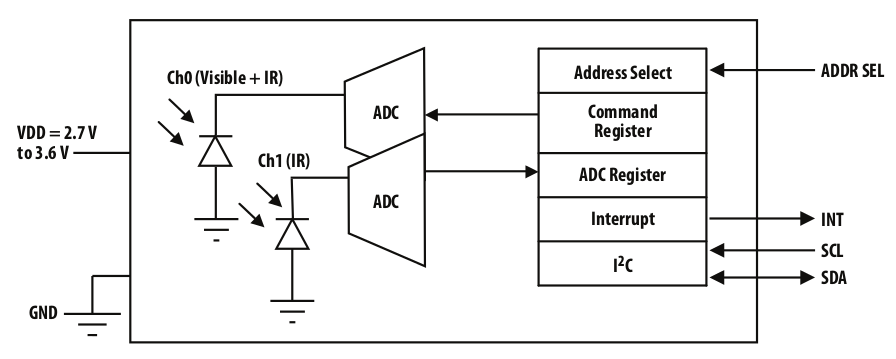
\includegraphics[width=0.65\linewidth]{./blockdiag}
\caption{Diagramma a blocchi}
\end{figure}
\end{textblock}

\begin{textblock}{12}(5.9,3.8)
\begin{figure}
\centering
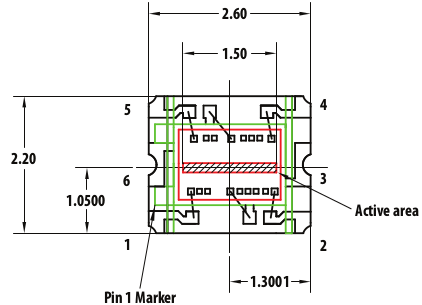
\includegraphics[width=0.55\linewidth]{./device}
\caption{Configurazione pin e \\ dimensioni (in mm)}
\label{fig:resp}
\end{figure}
\end{textblock}
\end{frame}


\begin{frame}{Caratteristiche operazionali}
\begin{textblock}{2}(0.40,3.6)
\begin{tabular}{c|c|c|c}
\textbf{Parameter} & \textbf{Channel} & \textbf{Max Value} & \textbf{Conditions}\\
\hline
\multirow{4}*{ADC count value [counts]} & CH0 & 65535 & \multirow{2}*{$T_{int}$ $>$ 178 ms} \\ \cline{2-3}
					& CH1 & 65535    &   \\ \cline{2-4} %\cline{5-6}
                   & CH0 & 37177    &  \multirow{2}*{$T_{int}$ = 101 ms} \\ \cline{2-3}
                   & CH1 & 37177    &   \\ \cline{2-4}
\hline
\multirow{2}*{Irradiance responsivity } & CH0 & 27.5 & {$\lambda _p$ = 640 nm,} \\ \cline{2-3}
					& CH1 & 5.5    &   $T_{int}$ = 101 ms \\ \cline{2-4} %\cline{5-6}
\multirow{2}*{[$\frac{\textrm{counts}}{\mu \textrm{W} / \textrm{cm}^2}$]}& CH0 & 8.4    &  {$\lambda _p$ = 940 nm, } \\ \cline{2-3}
                   & CH1 & 6.9    &   $T_{int}$ = 101 ms \\ \cline{2-4} %\cline{6-6}
\hline
\multirow{2}*{Illuminance responsivity } & CH0 & 36 & Fluorescence light  \\ \cline{2-3}
					& CH1 & 4    & $T_{int}$ = 402 ms  \\ \cline{2-4} %\cline{5-6}
\multirow{2}*{[$\frac{\textrm{counts}}{ \textrm{lux}}$]}  & CH0 & 144    &  Fluorescence light \\ \cline{2-3}
                   & CH1 & 72    &  $T_{int}$ = 101 ms \\  %\cline{6-6}
\end{tabular}
\end{textblock}
\end{frame}


\begin{frame}
\begin{itemize}
\item È stato usato $T_{int}$ = 402 ms, dunque i valori massimi di illuminanza e irraggiamento rilevabili sono rispettivamente  1820 lux e 2383 $\frac{\textrm{W}}{\textrm{cm}^2}$ per CH0, 16383 lux e 11915 $\frac{\textrm{W}}{\textrm{cm}^2}$ per CH1.
\item Tramite protocollo $I^2C$ Arduino restituisce:
\begin{itemize}
\item Valori dei due canali;\\
\item Rapporto $\frac{CH1}{CH0}$;\\
\item Illuminanza in lux calcolata tramite funzione di calibrazione.
\end{itemize} 
\end{itemize}
\end{frame}

\begin{frame}{Funzione di calibrazione}
\begin{textblock}{11.5}(2,5)
\begin{tabular}{c|c}
\textbf{x = CH1/CH0} & \textbf{Sensor lux formula} \\ 
\hline 
0 $<$ x $\leq$ 0.50  & (0.0304 $\cdot$ CH0) – (0.062 $\cdot$ CH0 $\cdot $x$^{1.4}$ ) \\ 
\hline 
0.50 $<$ x $\leq$ 0.61 & (0.0224 $\cdot$ CH0) – (0.031 $\cdot$ CH1) \\ 
\hline 
0.61 $<$ x $\leq$ 0.80 & (0.0128 $\cdot$ CH0) – (0.0153 $\cdot$ CH1) \\ 
\hline 
0.80 $<$ x $\leq$ 1.30 & (0.00146 $\cdot$ CH0) – (0.00112 $\cdot$ CH1) \\ 
\hline 
x $\geq$ 1.30 & 0 \\ 
\end{tabular} 
\end{textblock}
\end{frame}

\begin{frame}{Responsività e curva di calibrazione}
\begin{textblock}{12}(-1.7,3.6)
\begin{figure}
\centering
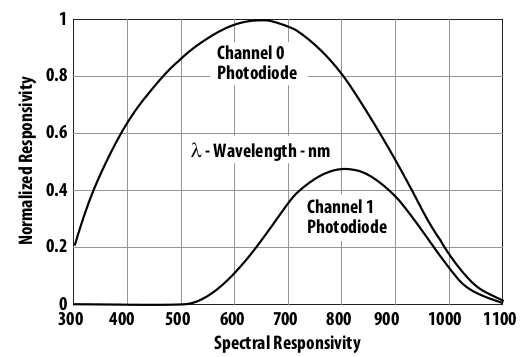
\includegraphics[width=0.6\linewidth]{./responsivity}
\caption{Curve di responsivita' spettrale}
\label{fig:resp}
\end{figure}
\end{textblock}


\begin{textblock}{11.5}(6.3,3.3)
\begin{figure}
\centering
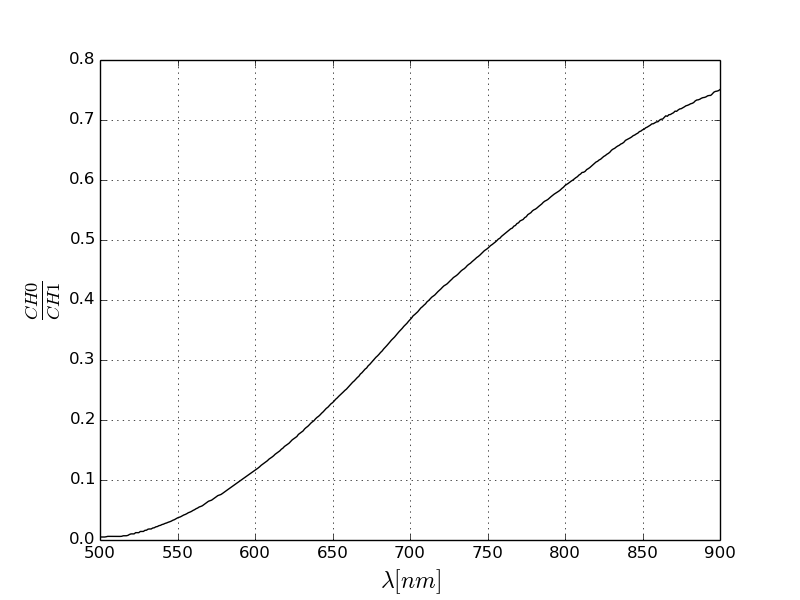
\includegraphics[width=0.6\linewidth]{./rapporto}
\caption{Curva di calibrazione}
\label{fig:cal}
\end{figure}
\end{textblock}
\end{frame}

\subsection{Prime misure}

\begin{frame}{Illuminazione stanza}
\begin{textblock}{9}(2.9,2.7)
\begin{figure}
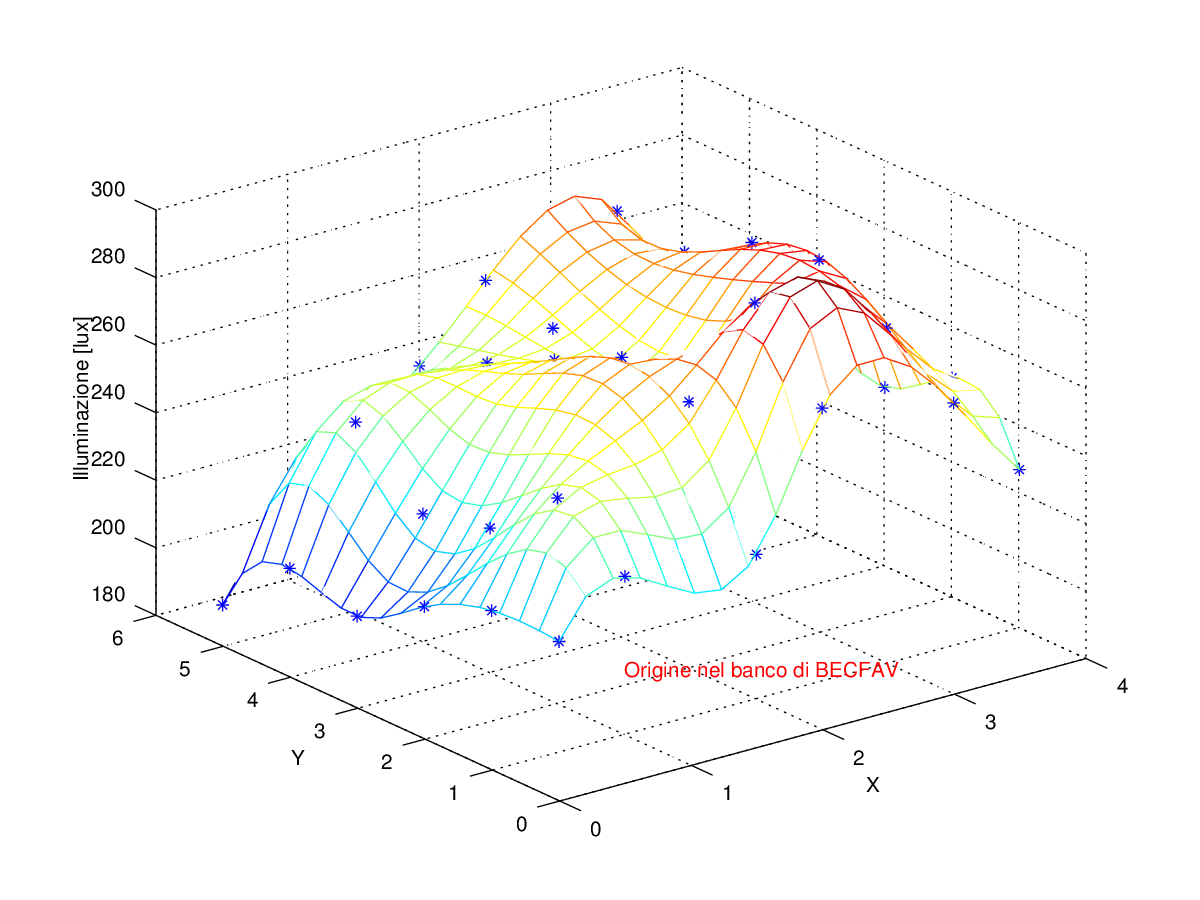
\includegraphics[scale=.4]{mesh}
\end{figure}
\end{textblock}
\end{frame}

\begin{frame}
\begin{itemize}
\item Grande luminosità in fondo perché vicino alle finestre;
\item Luci di destra sembrano più potenti di quelle di sinistra: PROVVEDERE!
\end{itemize}
\end{frame}

\begin{frame}{LED}
\begin{itemize}
\item 4 LED impiegati: HLMP-C115 (rosso), HLMP-C315 (giallo), LT3333 (verde), LB3333 (blu);\\
\item Resistenza di protezione di 470 $\Omega$;\\
\item LED schermati con rotolo di carta spesso: segnale nullo a LED spento
\end{itemize}
\end{frame}

\begin{frame}{HLMP-C115}
\begin{textblock}{9}(2.6,3.0)
\begin{figure}
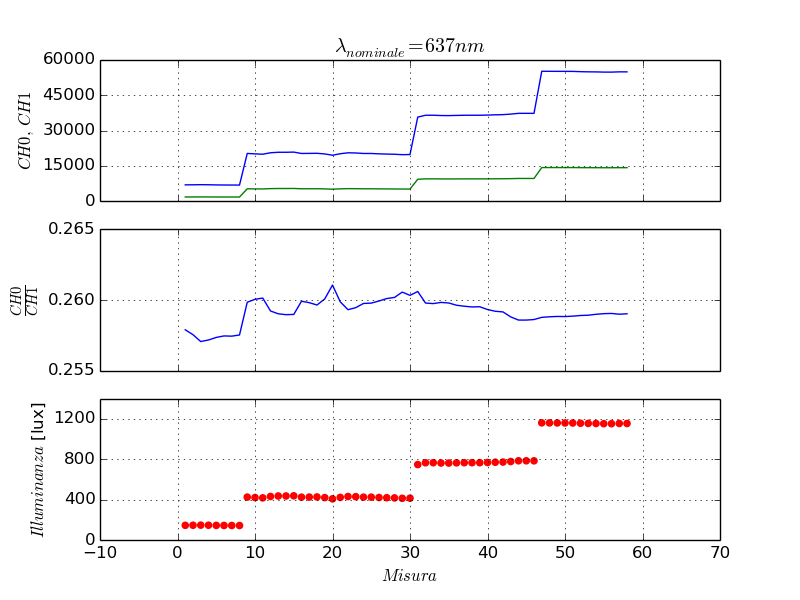
\includegraphics[scale=.42]{triple_rosso}
\end{figure}
\end{textblock}
\end{frame}

\begin{frame}{LT3333}
\begin{textblock}{9}(2.6,3.0)
\begin{figure}
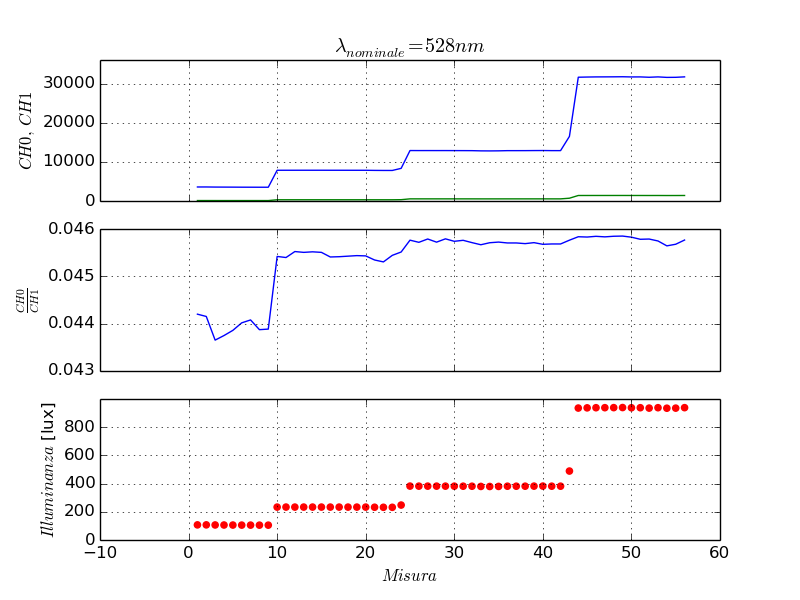
\includegraphics[scale=.42]{triple_verde}
\end{figure}
\end{textblock}
\end{frame}

\begin{frame}{Lunghezze d'onda vs Potenza}
\begin{textblock}{12}(-2,3.4)
\begin{figure}
\centering
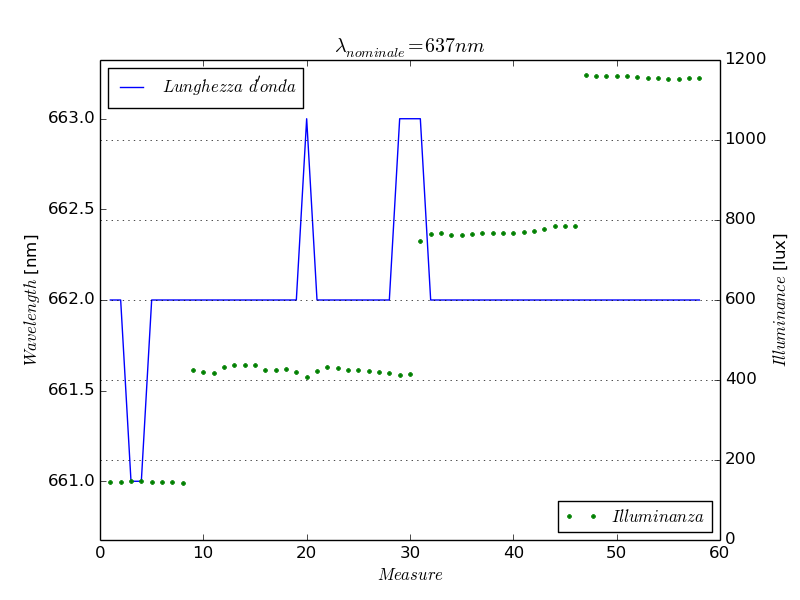
\includegraphics[width=0.6\linewidth]{./wave_hlmprosso_comp}
\caption{HLMP-C115}
\label{fig:resp}
\end{figure}
\end{textblock}


\begin{textblock}{12}(6,3.4)
\begin{figure}
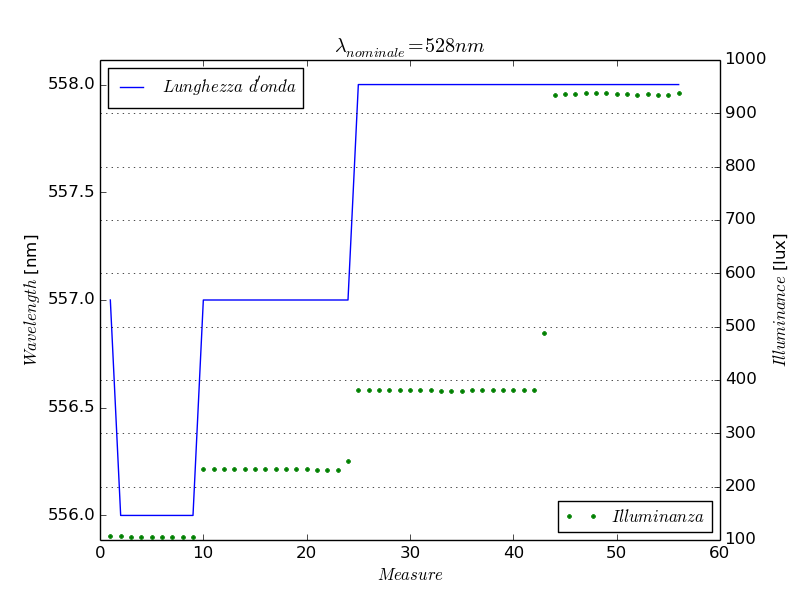
\includegraphics[width=0.6\linewidth]{./wave_led3333_comp}
\caption{LT3333}
\label{fig:cal}
\end{figure}
\end{textblock}
\end{frame}

\begin{frame}{Misure vs datasheet}
\begin{textblock}{11.5}(1.8,5)
\centering
\begin{tabular}{c|c|c}
LED & Valore misurato [nm] & Valore nominale [nm] \\ 
\hline 
HLMP-C115 & 662.1 $\pm$ 0.1 & 637 \\ 
\hline 
HLMP-C315 & 608.3 $\pm$ 0.2 & 585 \\ 
\hline 
LT3333 & 557.1 $\pm$ 0.2 & 528 \\ 
\hline 
LB3333 & 519 $\pm$ 1 & 470 \\
\end{tabular} 
\end{textblock}
\end{frame}

\begin{frame}{Prime Conclusioni}
\begin{itemize}
\item La lunghezza d'onda non dipende dall'intensità del LED;
\item Sovrastima delle lunghezze di 20-30 nm su tutti, 50 nm per il blu, di cui non abbiamo una spiegazione.
\end{itemize}
\end{frame}

\section{Misuratore analogico: WS-7.56-TO5}
\subsection{Caratterizzazione del dispositivo}

\begin{frame}
\begin{textblock}{10}(-2,3)
\begin{figure}
\centering
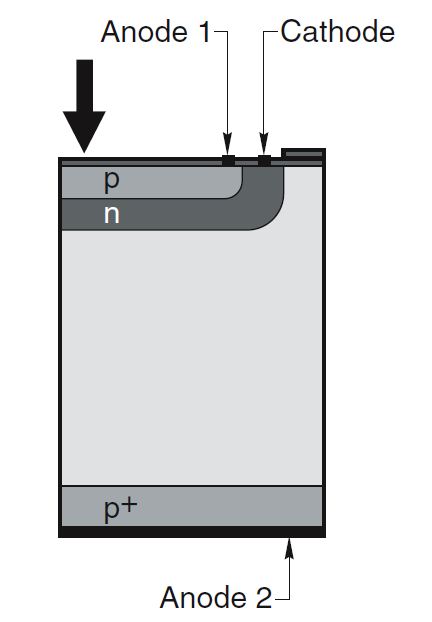
\includegraphics[width=0.4\linewidth]{./schema_analog_sensor}
\caption{$\, \, \, \, \, \, \,$Schema costruttivo \\
$\, \, \, \, \, \, \, \, \, \, \, \, \, \, \, \, \, \, \, \, \, \, \, \, \, \, \, \, \, \, \,$dei fotodiodi del WS-765-TO5.}
\label{fig:schema_analog_sensor}
\end{figure}
\end{textblock}

\begin{textblock}{7}(6,5)
\centering
\begin{tabular}{c|c}
\hline Area attiva & 7.56$mm^2$ \\ 
 Range operativo $\lambda$ & 450-900 nm \\ 
 Risoluzione spettrale & 0.01 nm \\ 
 Livello di saturazione & 150 $\mu$W @0V \\ 
  & 3mW @5V \\ 
 Dark current  & 100 nA Max\\ 
  & 10 nA Typ \\
 Rise time & 1-10 $\mu$s (Diodo1-Diodo2) \\
 
\hline
\end{tabular} 
\end{textblock}

\end{frame}

\begin{frame}{Responsività spettrale}
\begin{textblock}{10}(-1,4)
\begin{figure}
\centering
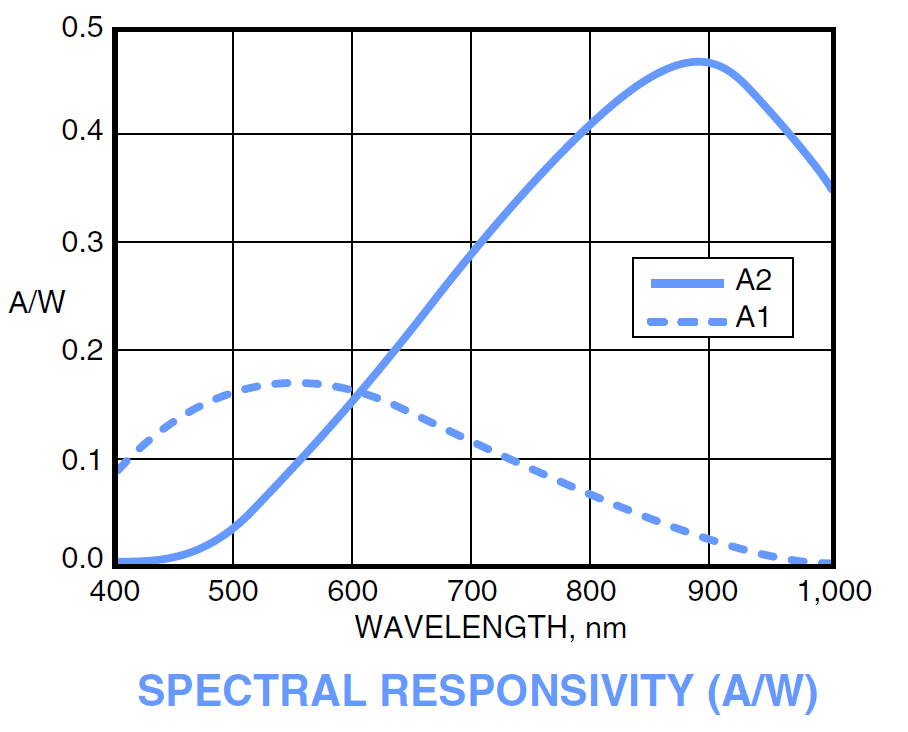
\includegraphics[width=0.6\linewidth]{./spectral_respo}
\caption{Curva di responsività \\
spettrale.}
\label{fig:spectral_resp}
\end{figure}
\end{textblock}

\begin{textblock}{10}(6,4)
\begin{figure}
\centering
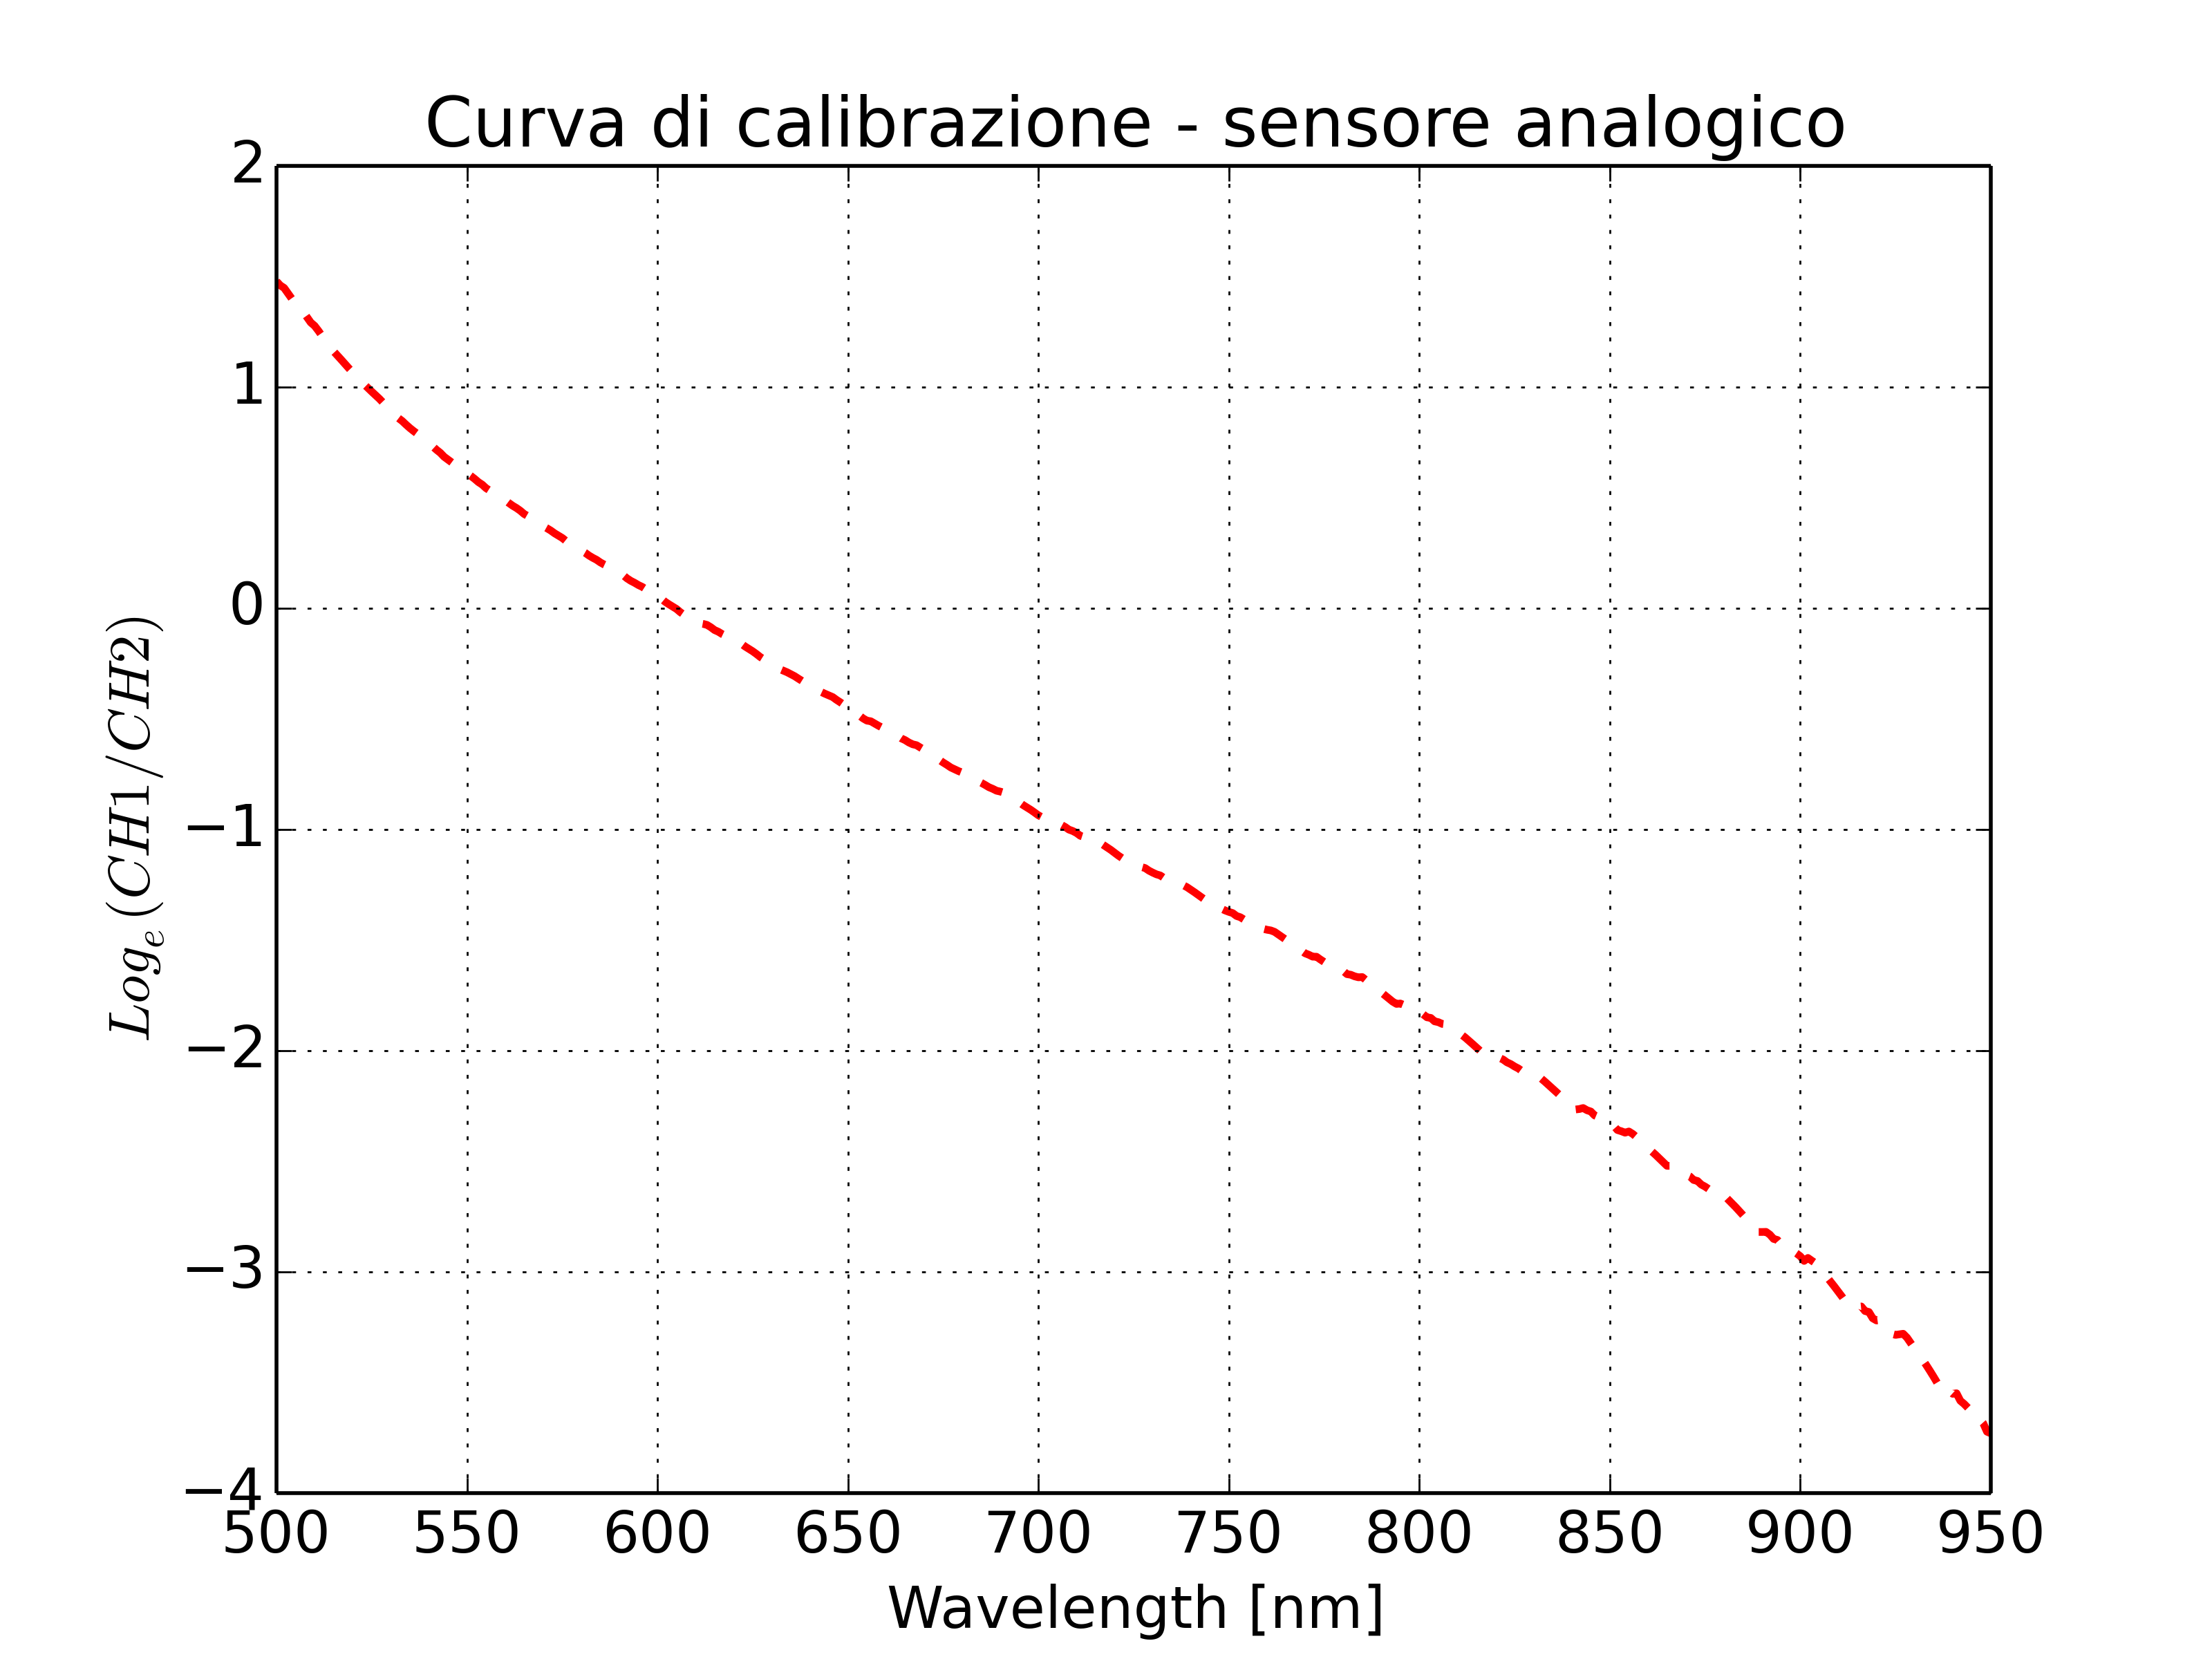
\includegraphics[width=0.6\linewidth]{./calibrazione_analog}
\caption{Curva di calibrazione \\
logaritmo del quoziente.}
\label{fig:calibr_logaritmo}
\end{figure}
\end{textblock}

\end{frame}

\begin{frame}{Montaggio e dimensionamento}
\begin{figure}
\centering
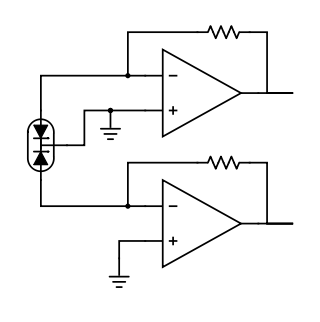
\includegraphics[width=0.3\linewidth]{./analog_scheme}
%\caption{Schema di montaggio della coppia di fotodiodi del WS-756-TO5}
%\label{fig:schema_montaggio}
\end{figure}

\fontsize{10}{12}
\begin{itemize}
\item Circuito con due op-amp in modalità invertente
\item Due transimpedenze uguali nei limiti dell'errore 
\item Per dimensionare le trans-impedenze si considera la curva di responsività: l'ordine di grandezza della corrente è 10-100 $\mu$A, resistenze a trans-impedenza dell'ordine del centinaio di k$\Omega$
\item $R_1 = 82.3 k\Omega$ e $R_2 = 82.2 k\Omega$ (prima) e $R_1 = 219 k\Omega$ e $R_2 = 220 k\Omega$ (poi).
\end{itemize}
\end{frame}

\begin{frame}{ENEL}

\begin{textblock}{12}(-1,3)
\begin{figure}
%\centering\\all'illuminazione \\della stanza. CH2 piccato sul rosso.
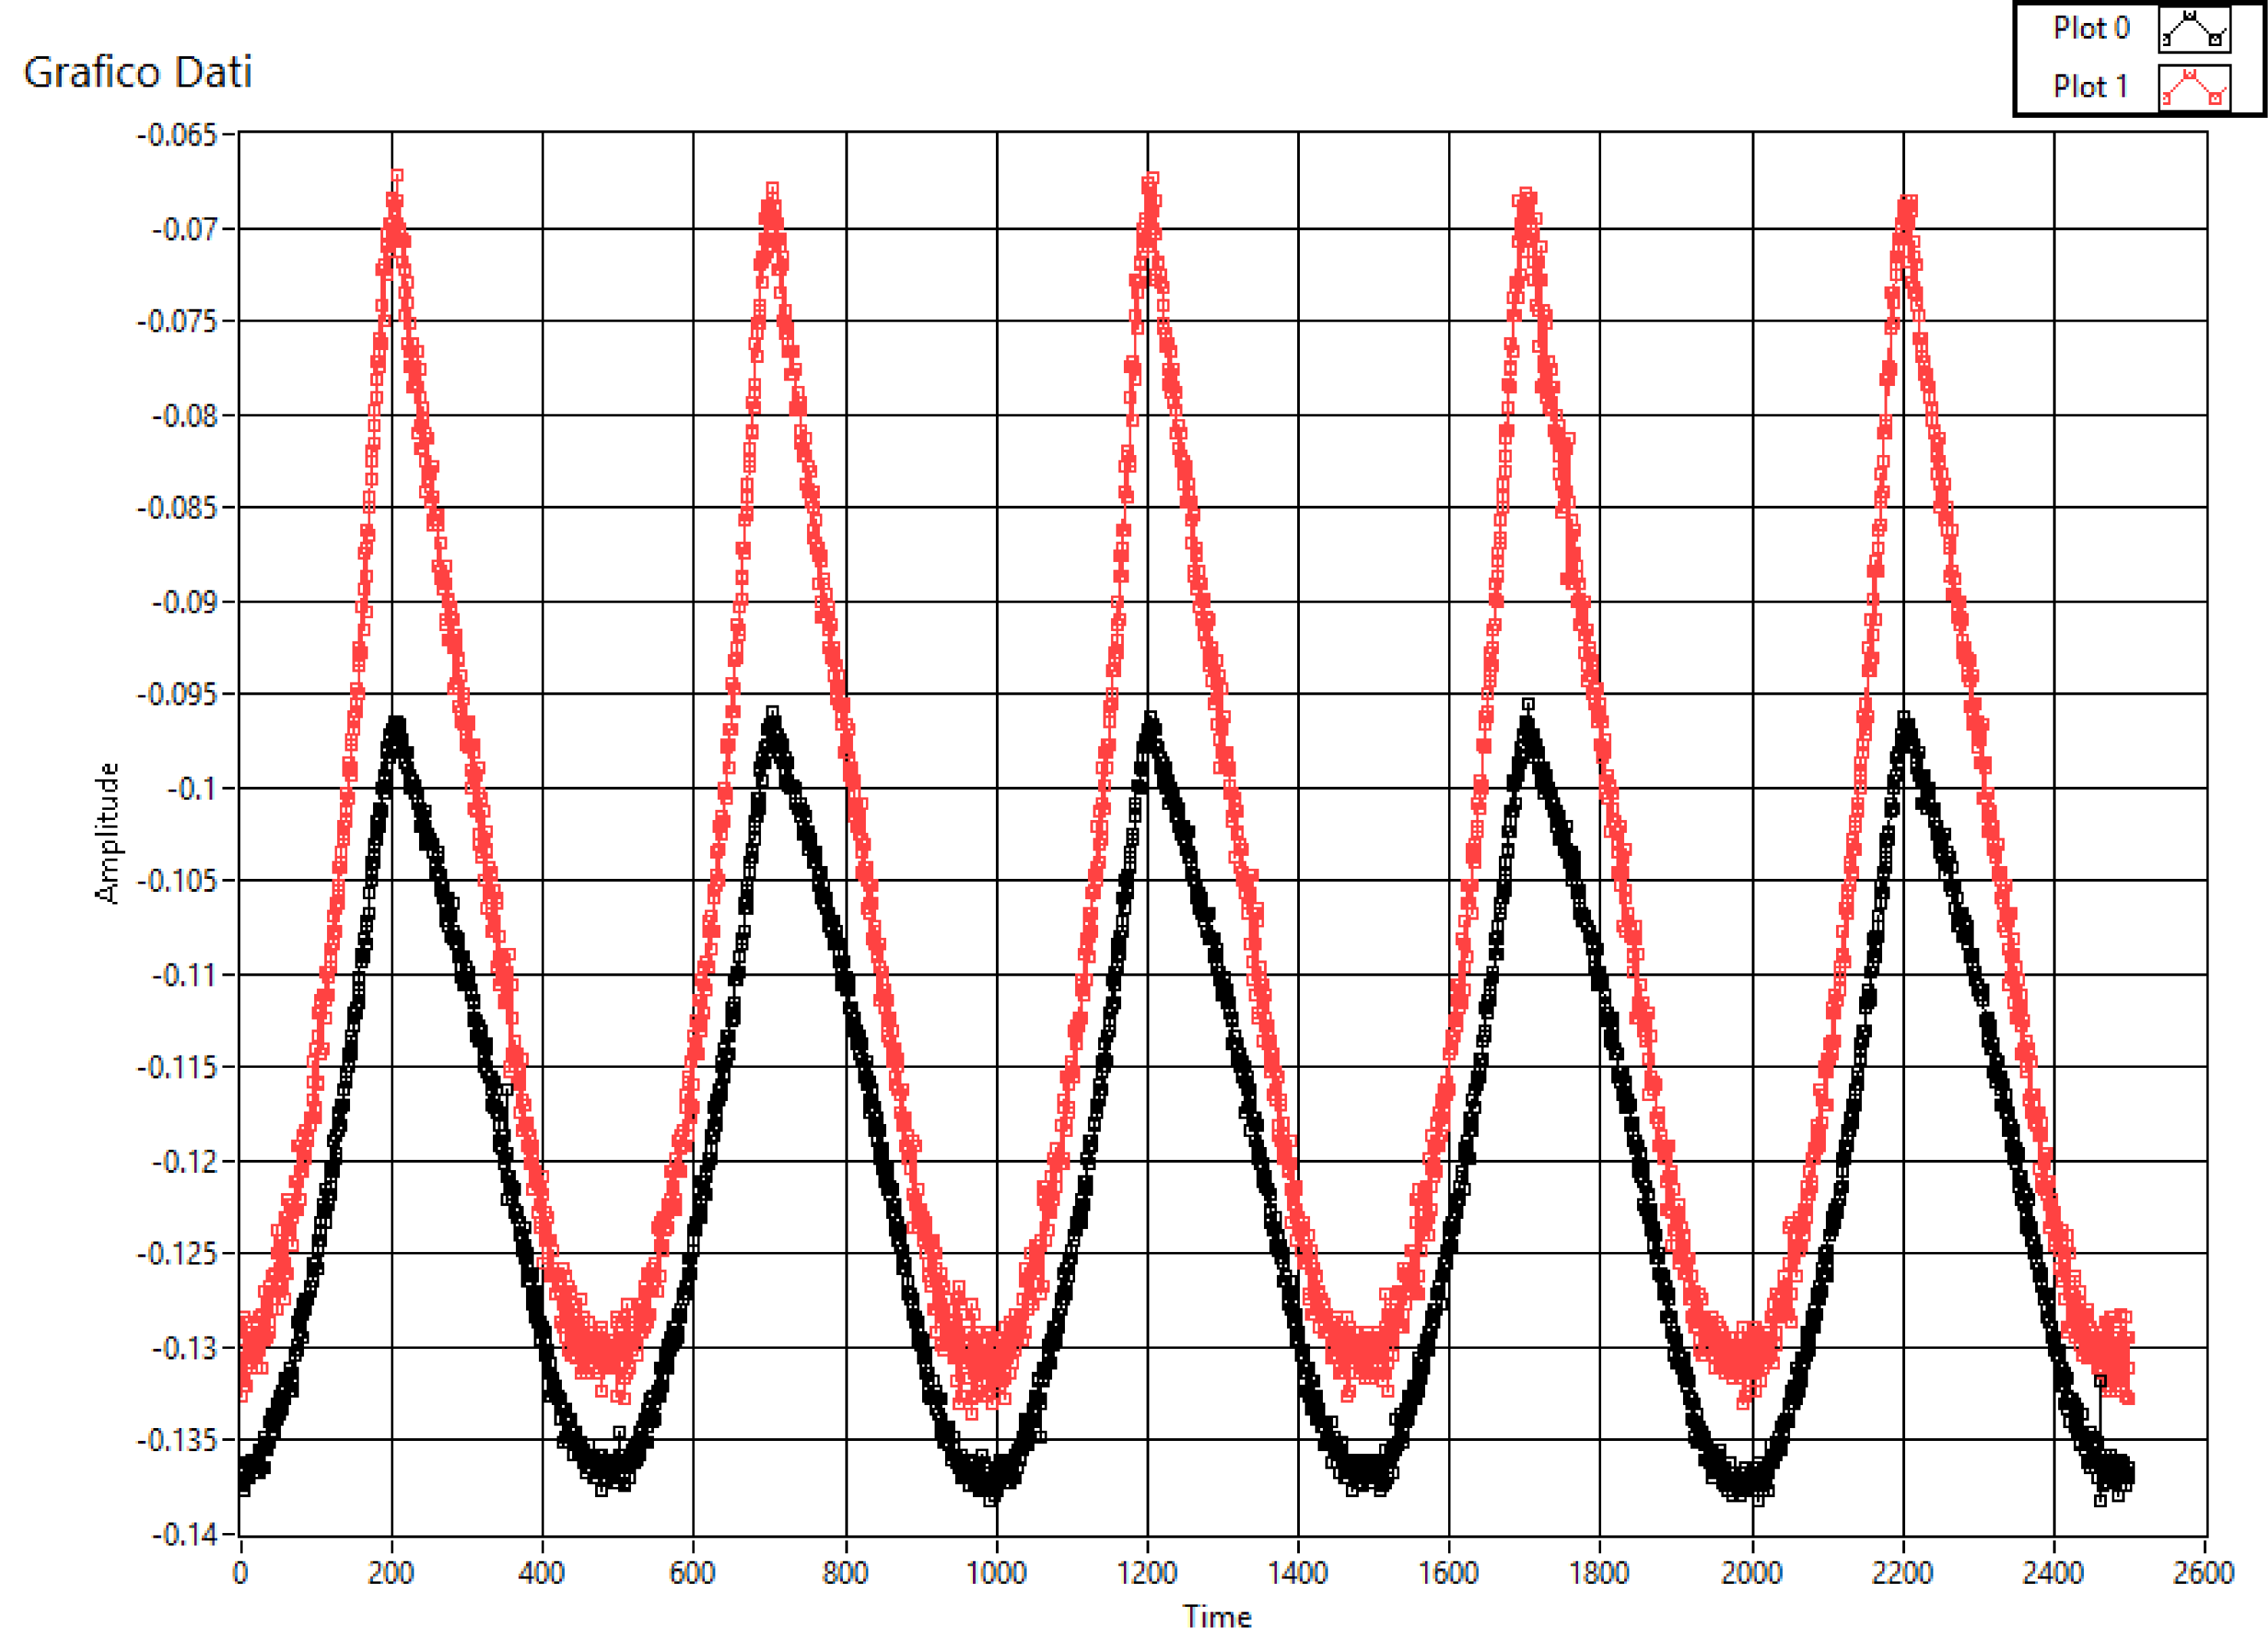
\includegraphics[width=0.5\linewidth]{./luce_stanza_enel}
\caption{Segnale relativo\\
all'illuminazione stanza.}
\label{fig:enel}
\end{figure}
\end{textblock}

\begin{textblock}{12}(6,3)
\begin{figure}
\centering
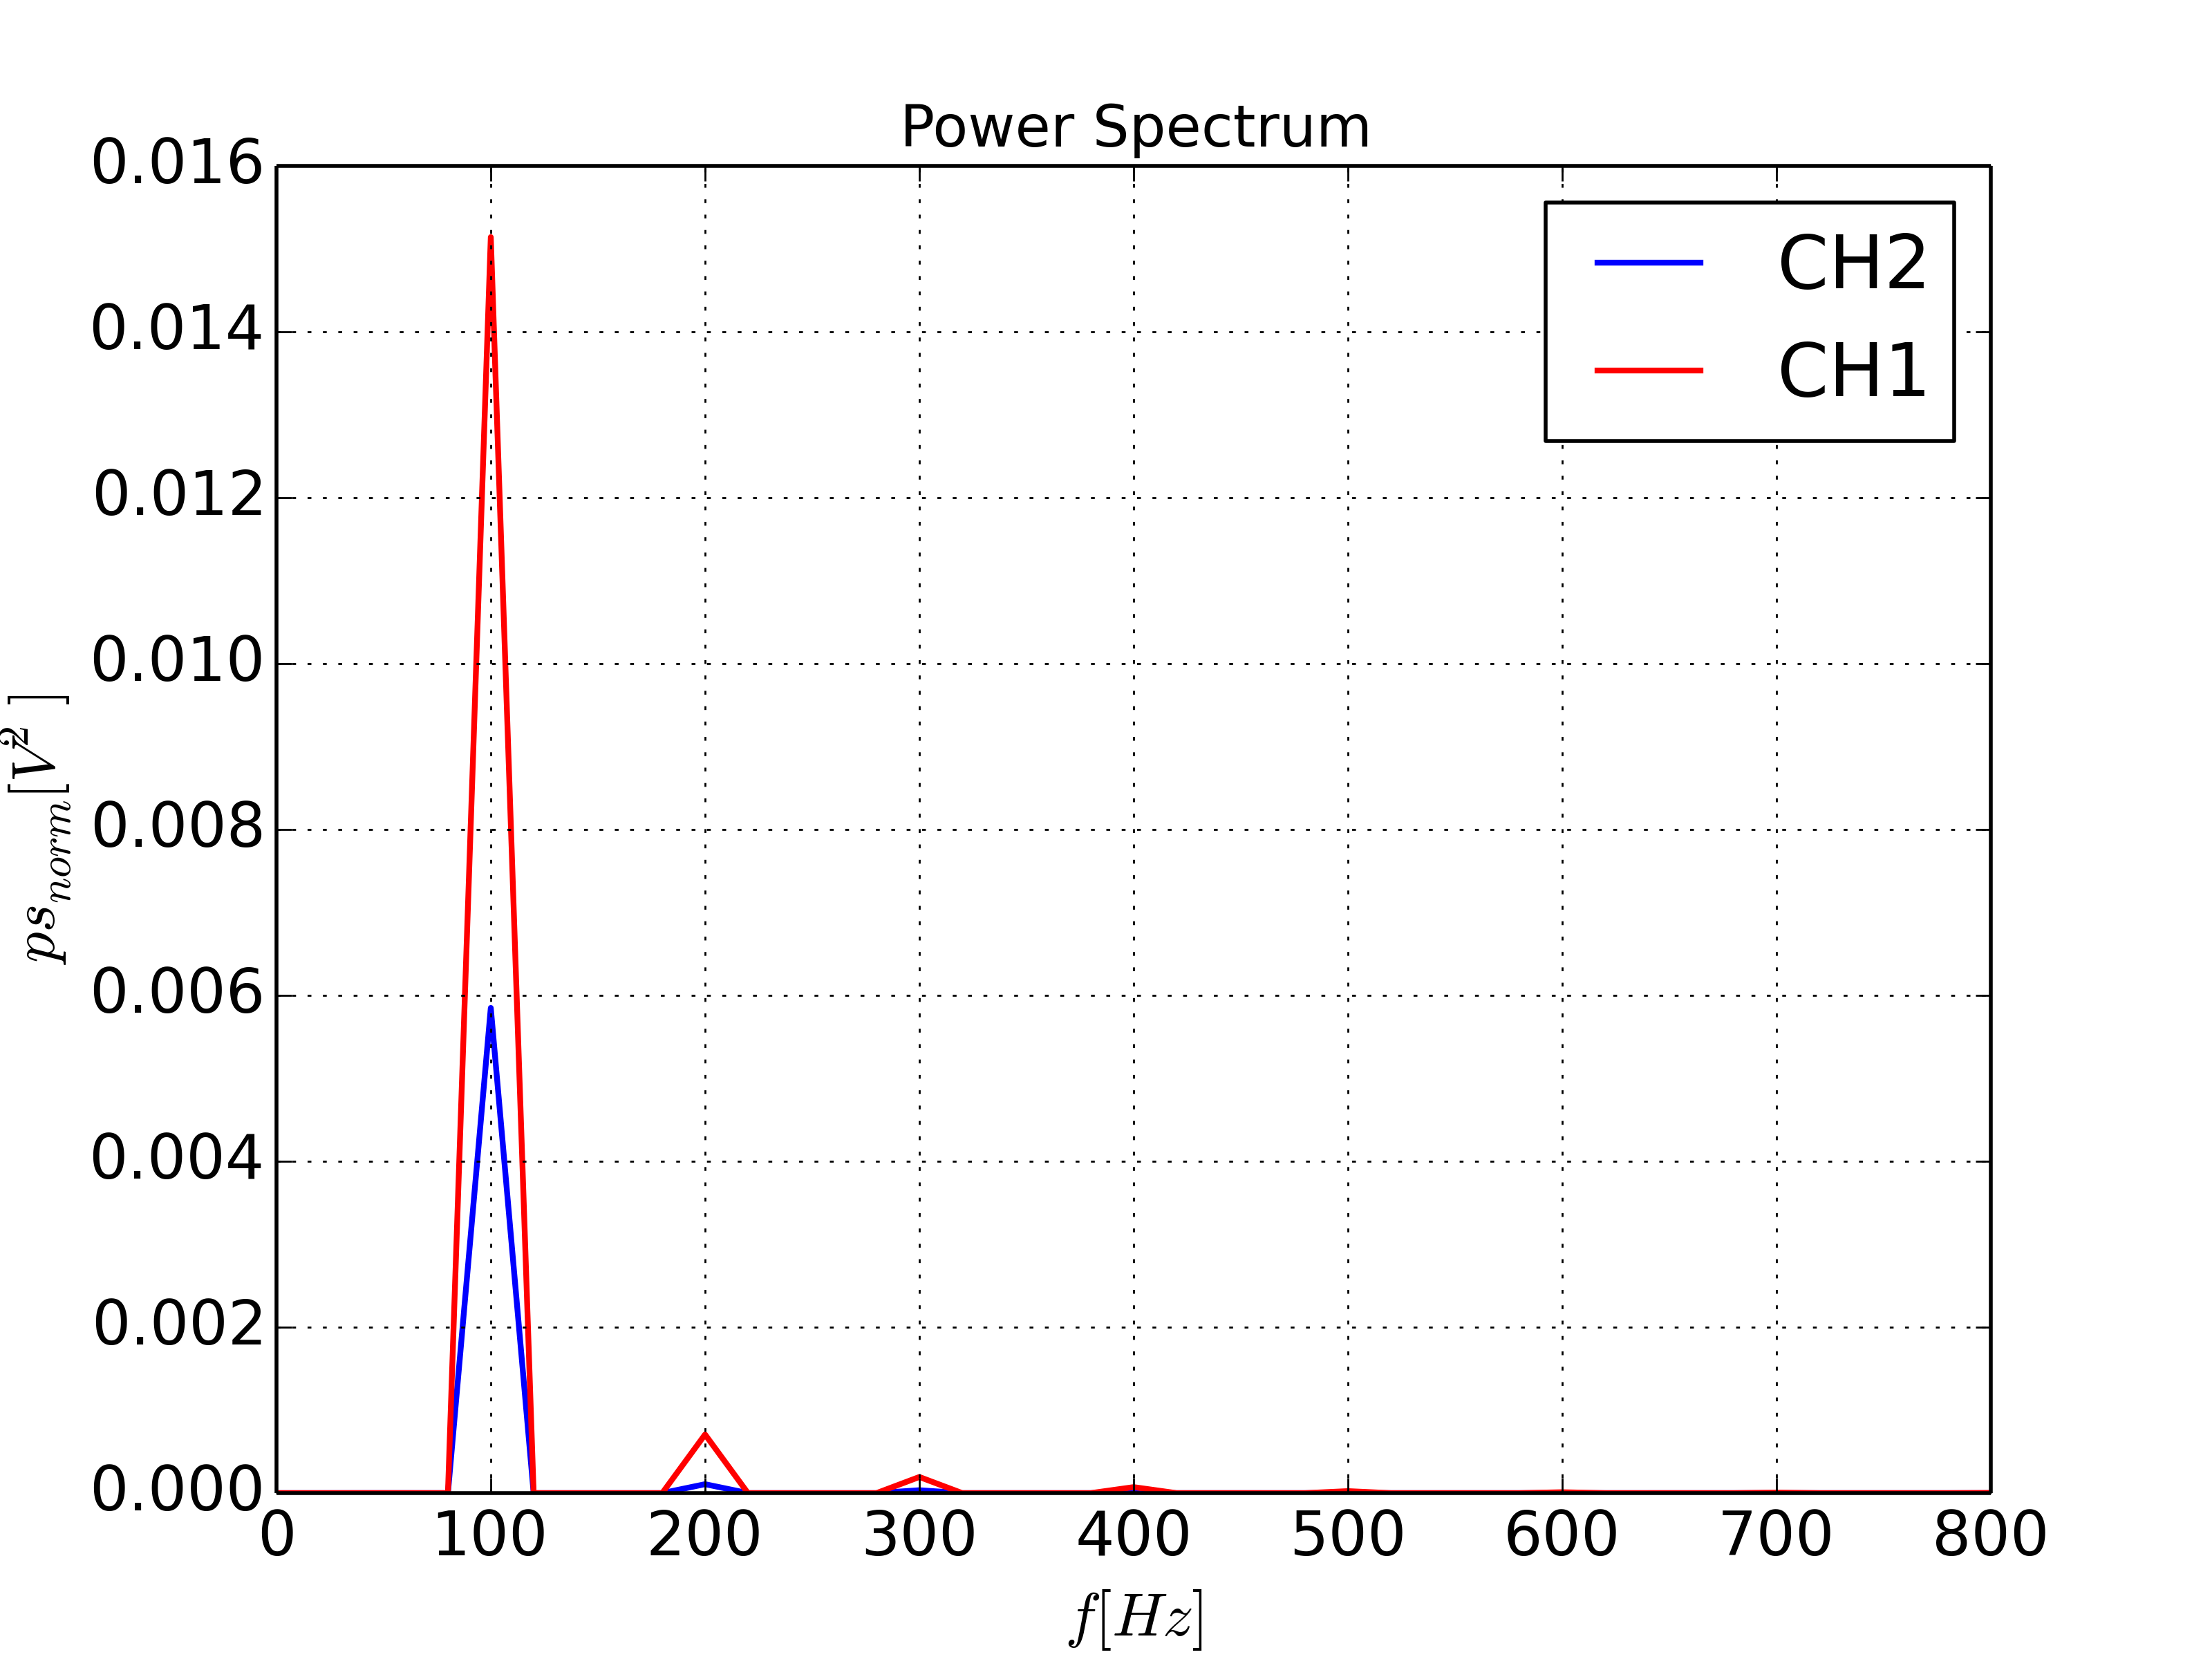
\includegraphics[width=0.5\linewidth]{./fft_lucestanza}
\caption{Fast Fourier transform \\
del segnale di luce ambientale.}
\label{fig:fft_lucestanza}
\end{figure}
\end{textblock}

\begin{textblock}{10}(3,13)
CH2 piccato sul rosso.
\end{textblock}

\end{frame}

\begin{frame}{Segnale di \textit{buio}}
In condizioni di \textit{buio} la risposta in tensione è diversa da zero per entrambi i fotodiodi: valore medio \textbf{positivo} $\sim$ a 7-8mV.\\
Ipotesi:
\begin{itemize}
\item \underline{Non} si tratta della \textit{dark current}, corrente di ricombinazione: la $I_D$ scorre dal catodo all'anodo, così come la fotocorrente in modalità di funzionamento fotovoltaica. La tensione sarebbe dello stesso segno.

\item L'input offset current del \textsc{$\mu$a741cp}: valore tipico  20nA alle nostre condizioni di lavoro, potrebbe essere responsabile di $\sim 5$mV.
\end{itemize}

Nelle misure successive si è cercato di rilevare tensioni di almeno 1-2 ordini di grandezza maggiori.
\end{frame}

\subsection{Caratterizzazione di un LED}
\begin{frame}{LED impiegati}
\begin{table}[h]
\centering
\fontsize{10}{12}
% This LaTeX table template is generated by emacs 24.3.1
\begin{tabular}{l|c|c|c}
\hline
\textbf{LED} & \textbf{Wavelength} datasheet (nm) & $log(CH1/CH2)$ & $\delta log$ \\
\hline
\textsc{hlmpd101-645} & 645 & -0.539 & 0.006 \\
\textsc{hlmpc115-red} & 637 & -0.522 & 0.003 \\
\textsc{hlmpc315-Y} & 585 & 0.172 & 0.006 \\
\textsc{la3366} & 615 & -0.101 & 0.003 \\
\textsc{lb3333} & 470 & 2.26 & 0.02 \\
\textsc{led450} & 450 & 2.87 & 0.02 \\
\textsc{lo3336} & 606 & -0.101 & 0.002 \\
\textsc{lpk376} & 560 & 0.65 & 0.04 \\
\textsc{ls3336} & 633 & -0.332 & 0.001 \\
\textsc{lt3333} & 528 & 0.908 & 0.01 \\
\textsc{ly3336} & 587 & 0.209 & 0.001 \\
\textsc{sfh4873-880} & 880 & -2.439 & 0.004 \\
\textsc{ssl-lxa} & 660 & -0.58 & 0.02 \\
\textsc{tshg8400-830} & 830 & -1.964 & 0.007 \\
\hline
\end{tabular}
\caption{title}
\label{tabella_LED}
\end{table}
\end{frame}

\begin{frame}{Lunghezze d'onda (datasheet) e curva di calibrazione}
\begin{figure}
\centering
\subfloat[LED ($\lambda$ datasheet) sulla curva di calibrazione del sensore analogico.]{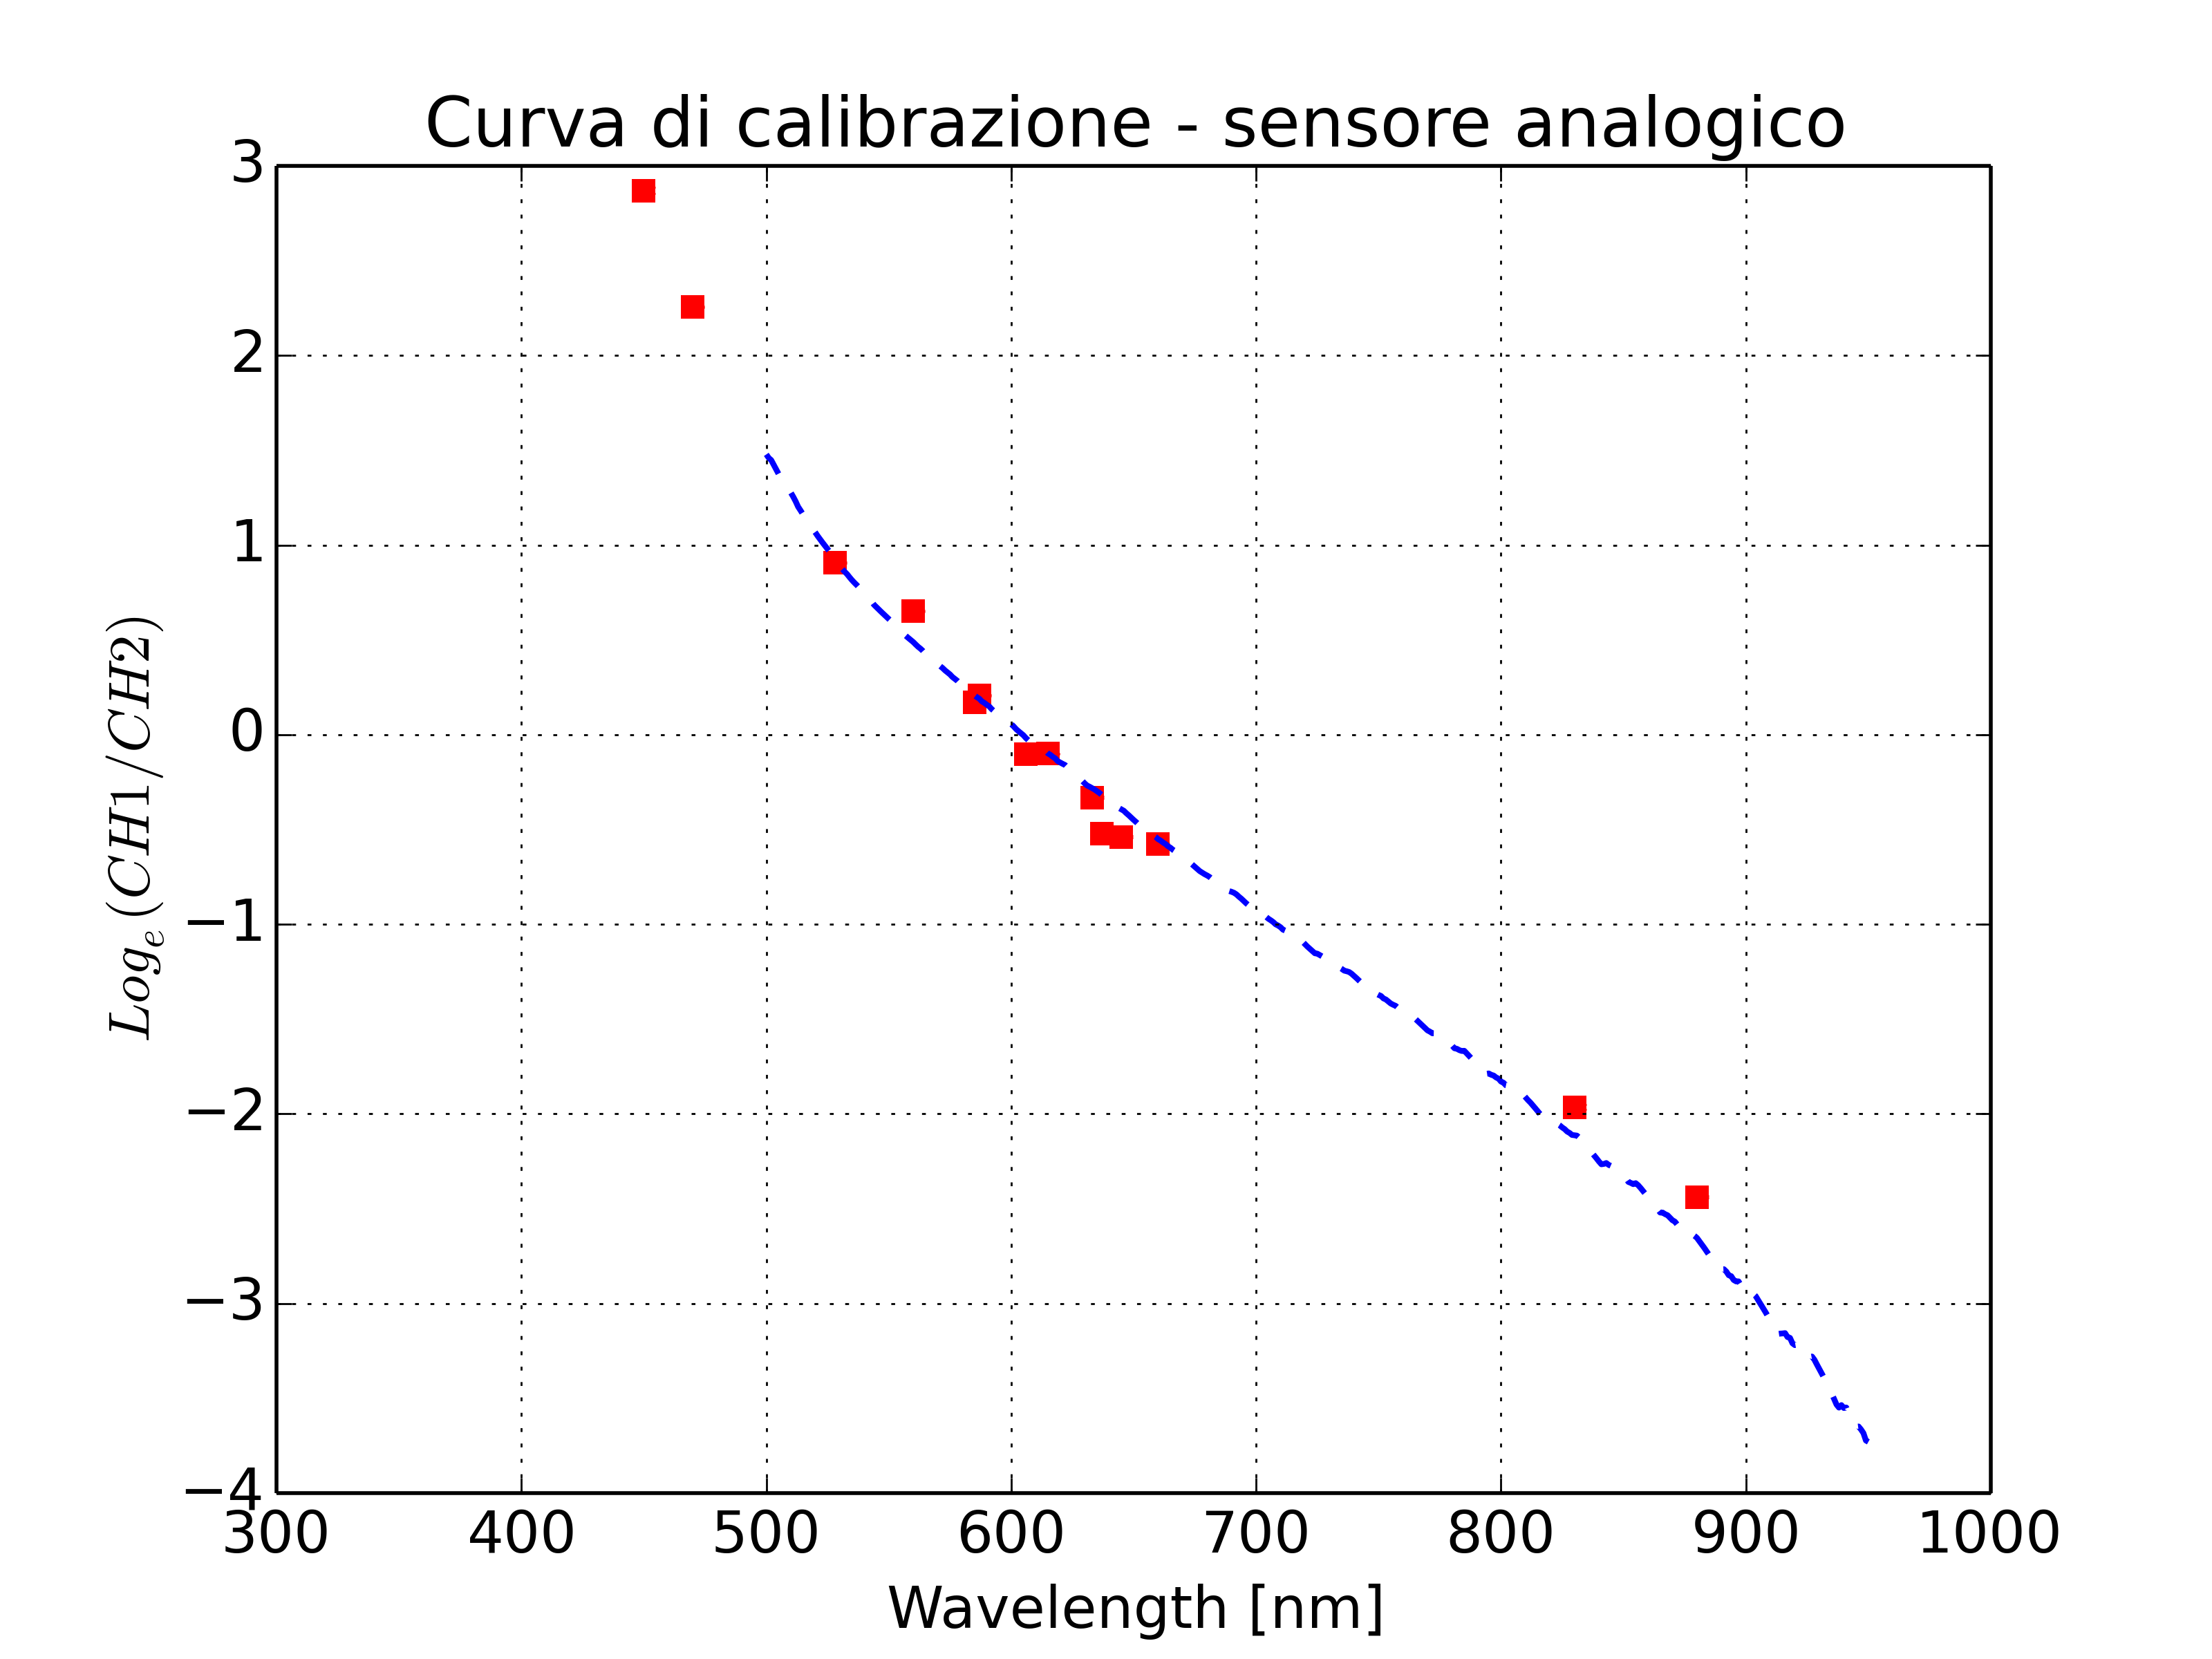
\includegraphics[width=0.4\linewidth]{./calibrazione_led}

\label{fig:calibrazione_led}}
\subfloat[Scarto fra $\lambda$ datasheet e "calibrazione" (interpolate) per ciascun LED.]{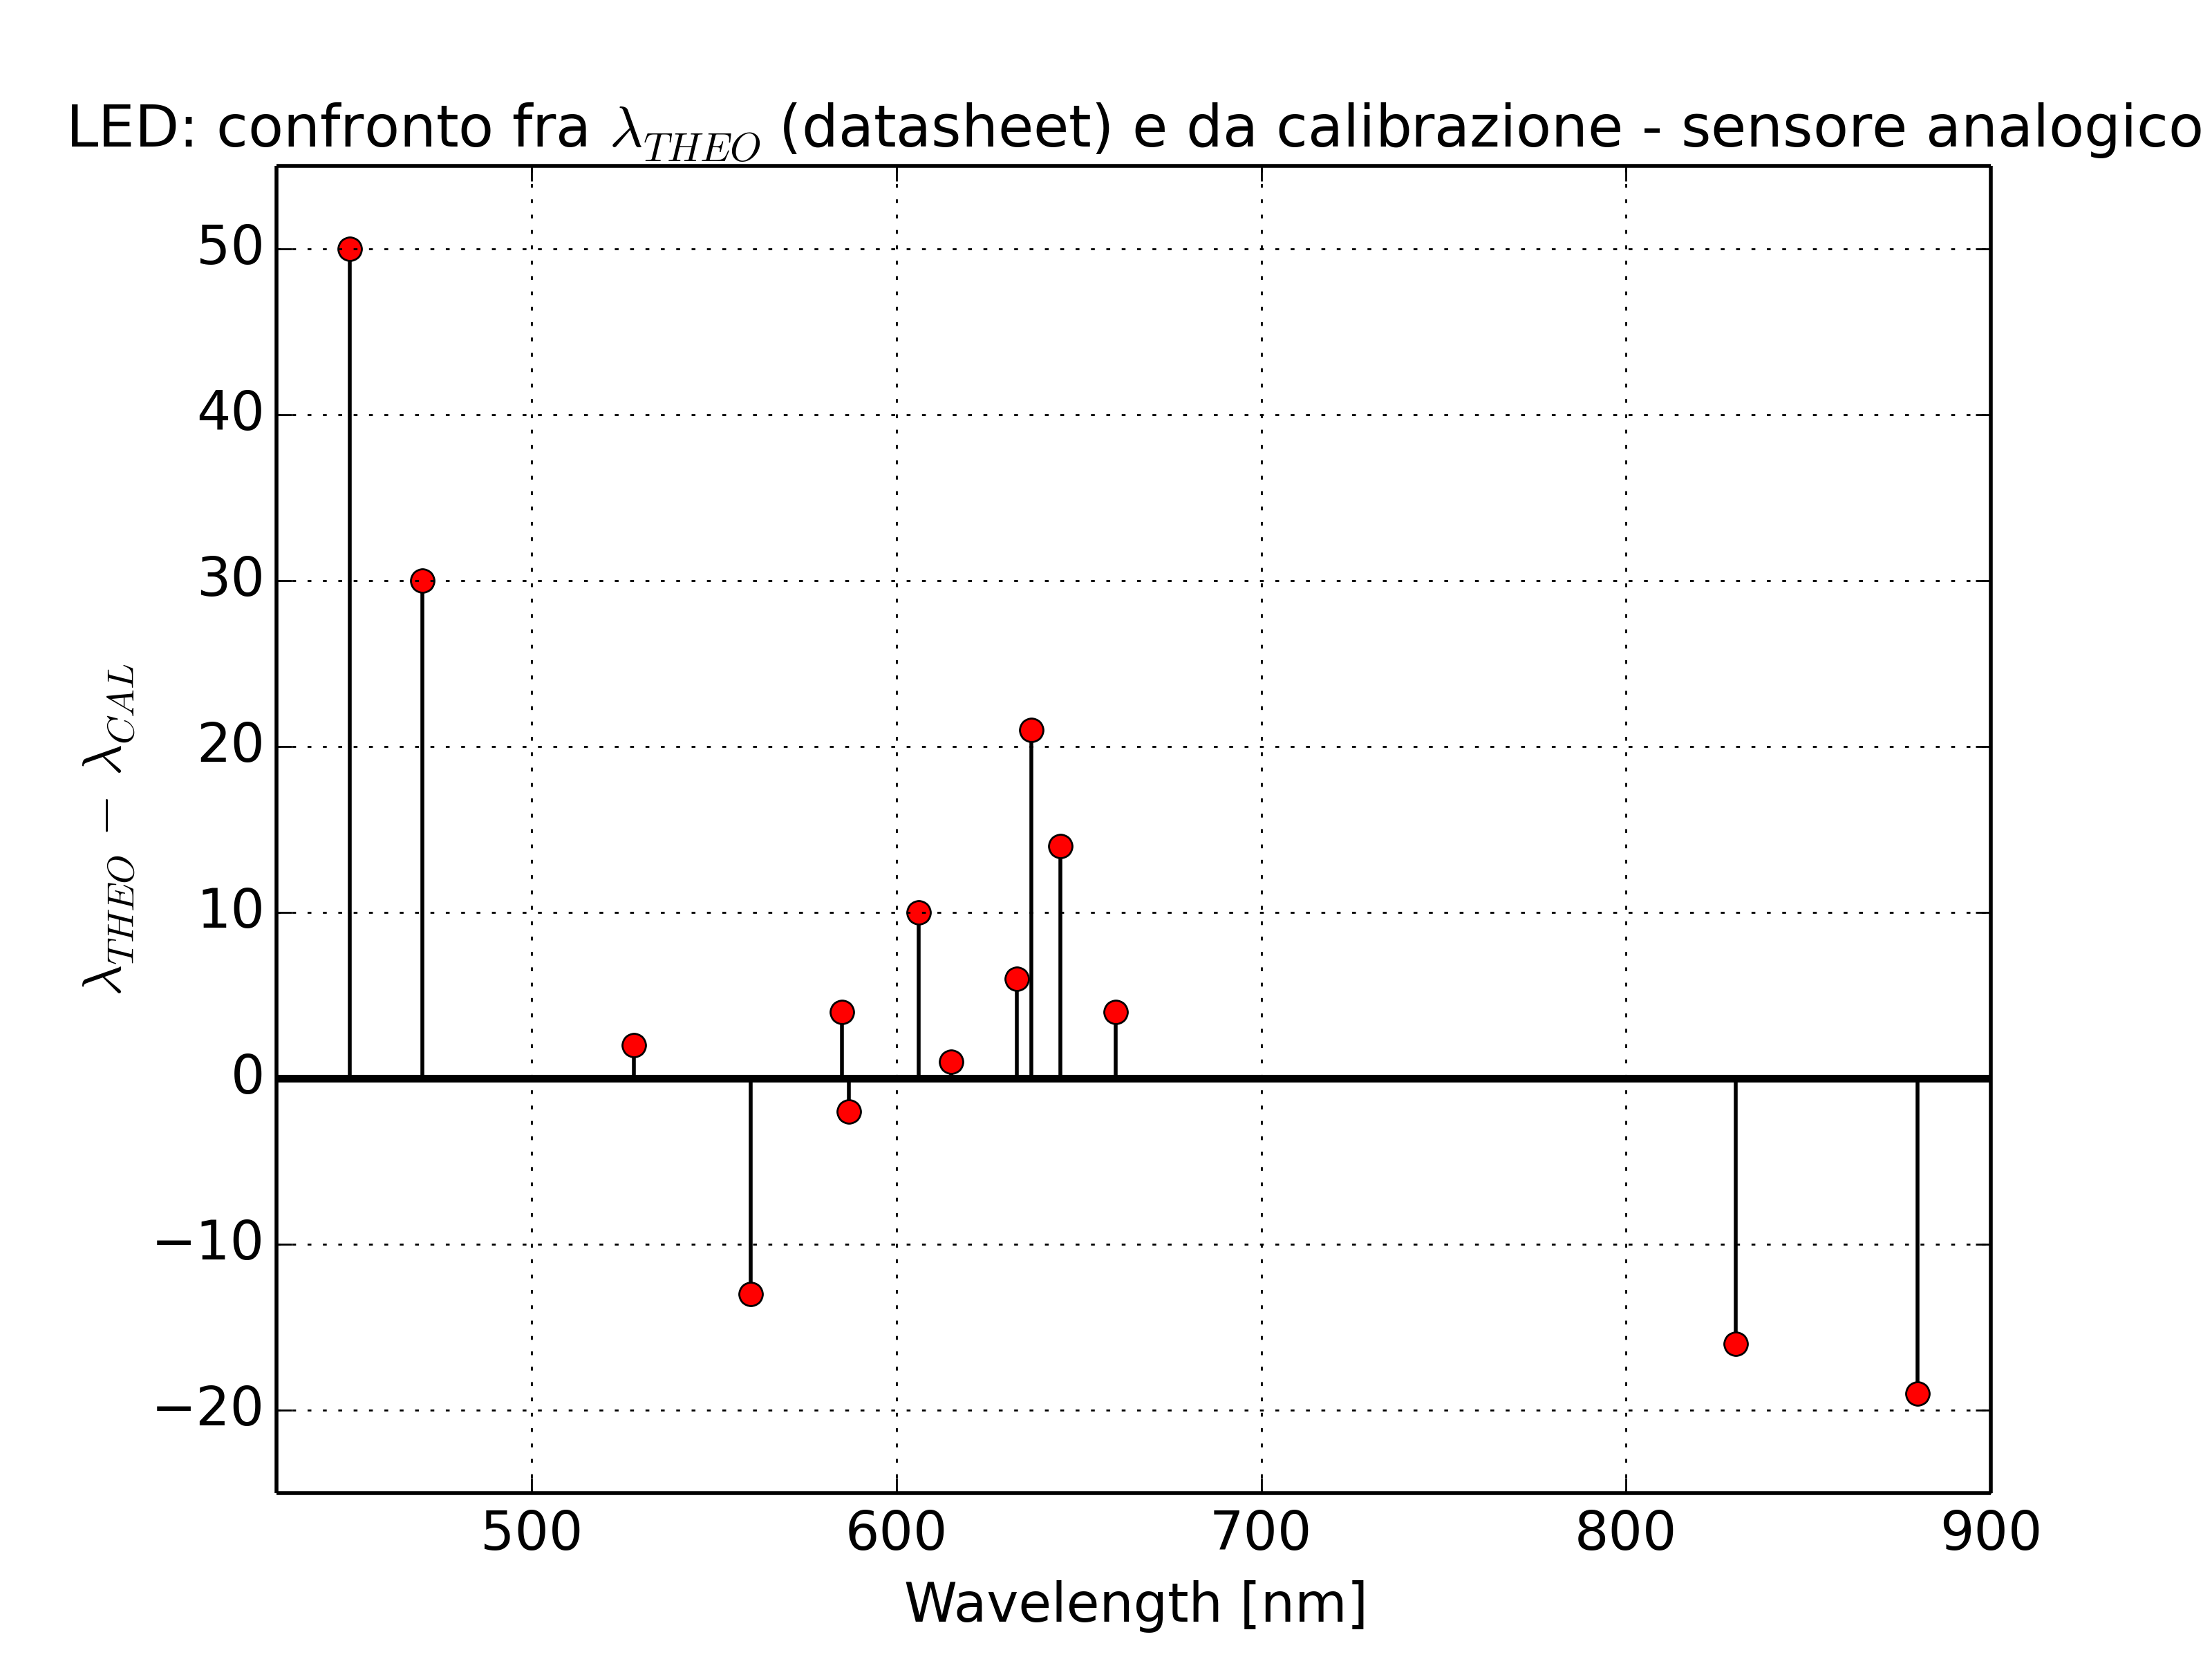
\includegraphics[width=0.4\linewidth]{./LED_confronto}
\label{fig:LED_confronto}}

\end{figure}


\begin{itemize}
\item Per i LED nel blu, la curva di calibrazione non copre valori di interesse.
\end{itemize}

\end{frame}

\begin{frame}{Estrapolazione della curva}
\fontsize{9}{11}
Vogliamo avere a disposizione dei valori attendibili nella regione 450-500nm.
\begin{itemize}
\item Per mezzo di Octave cerchiamo un polinomio interpolatore dei punti di calibrazione e prolunghiamolo per $\lambda$ fra 450-500nm. \item Funzione di interpolazione: \textsc{polyfit}. Di che grado? Comportamento estremamente variabile.
\item Ci aiutiamo modellizzando le curve di responsività come gaussiane.
\end{itemize}


\begin{figure}
\centering
\subfloat[Modellizzazione della curva di responsività: la curva in rosso è il log del rapporto.]{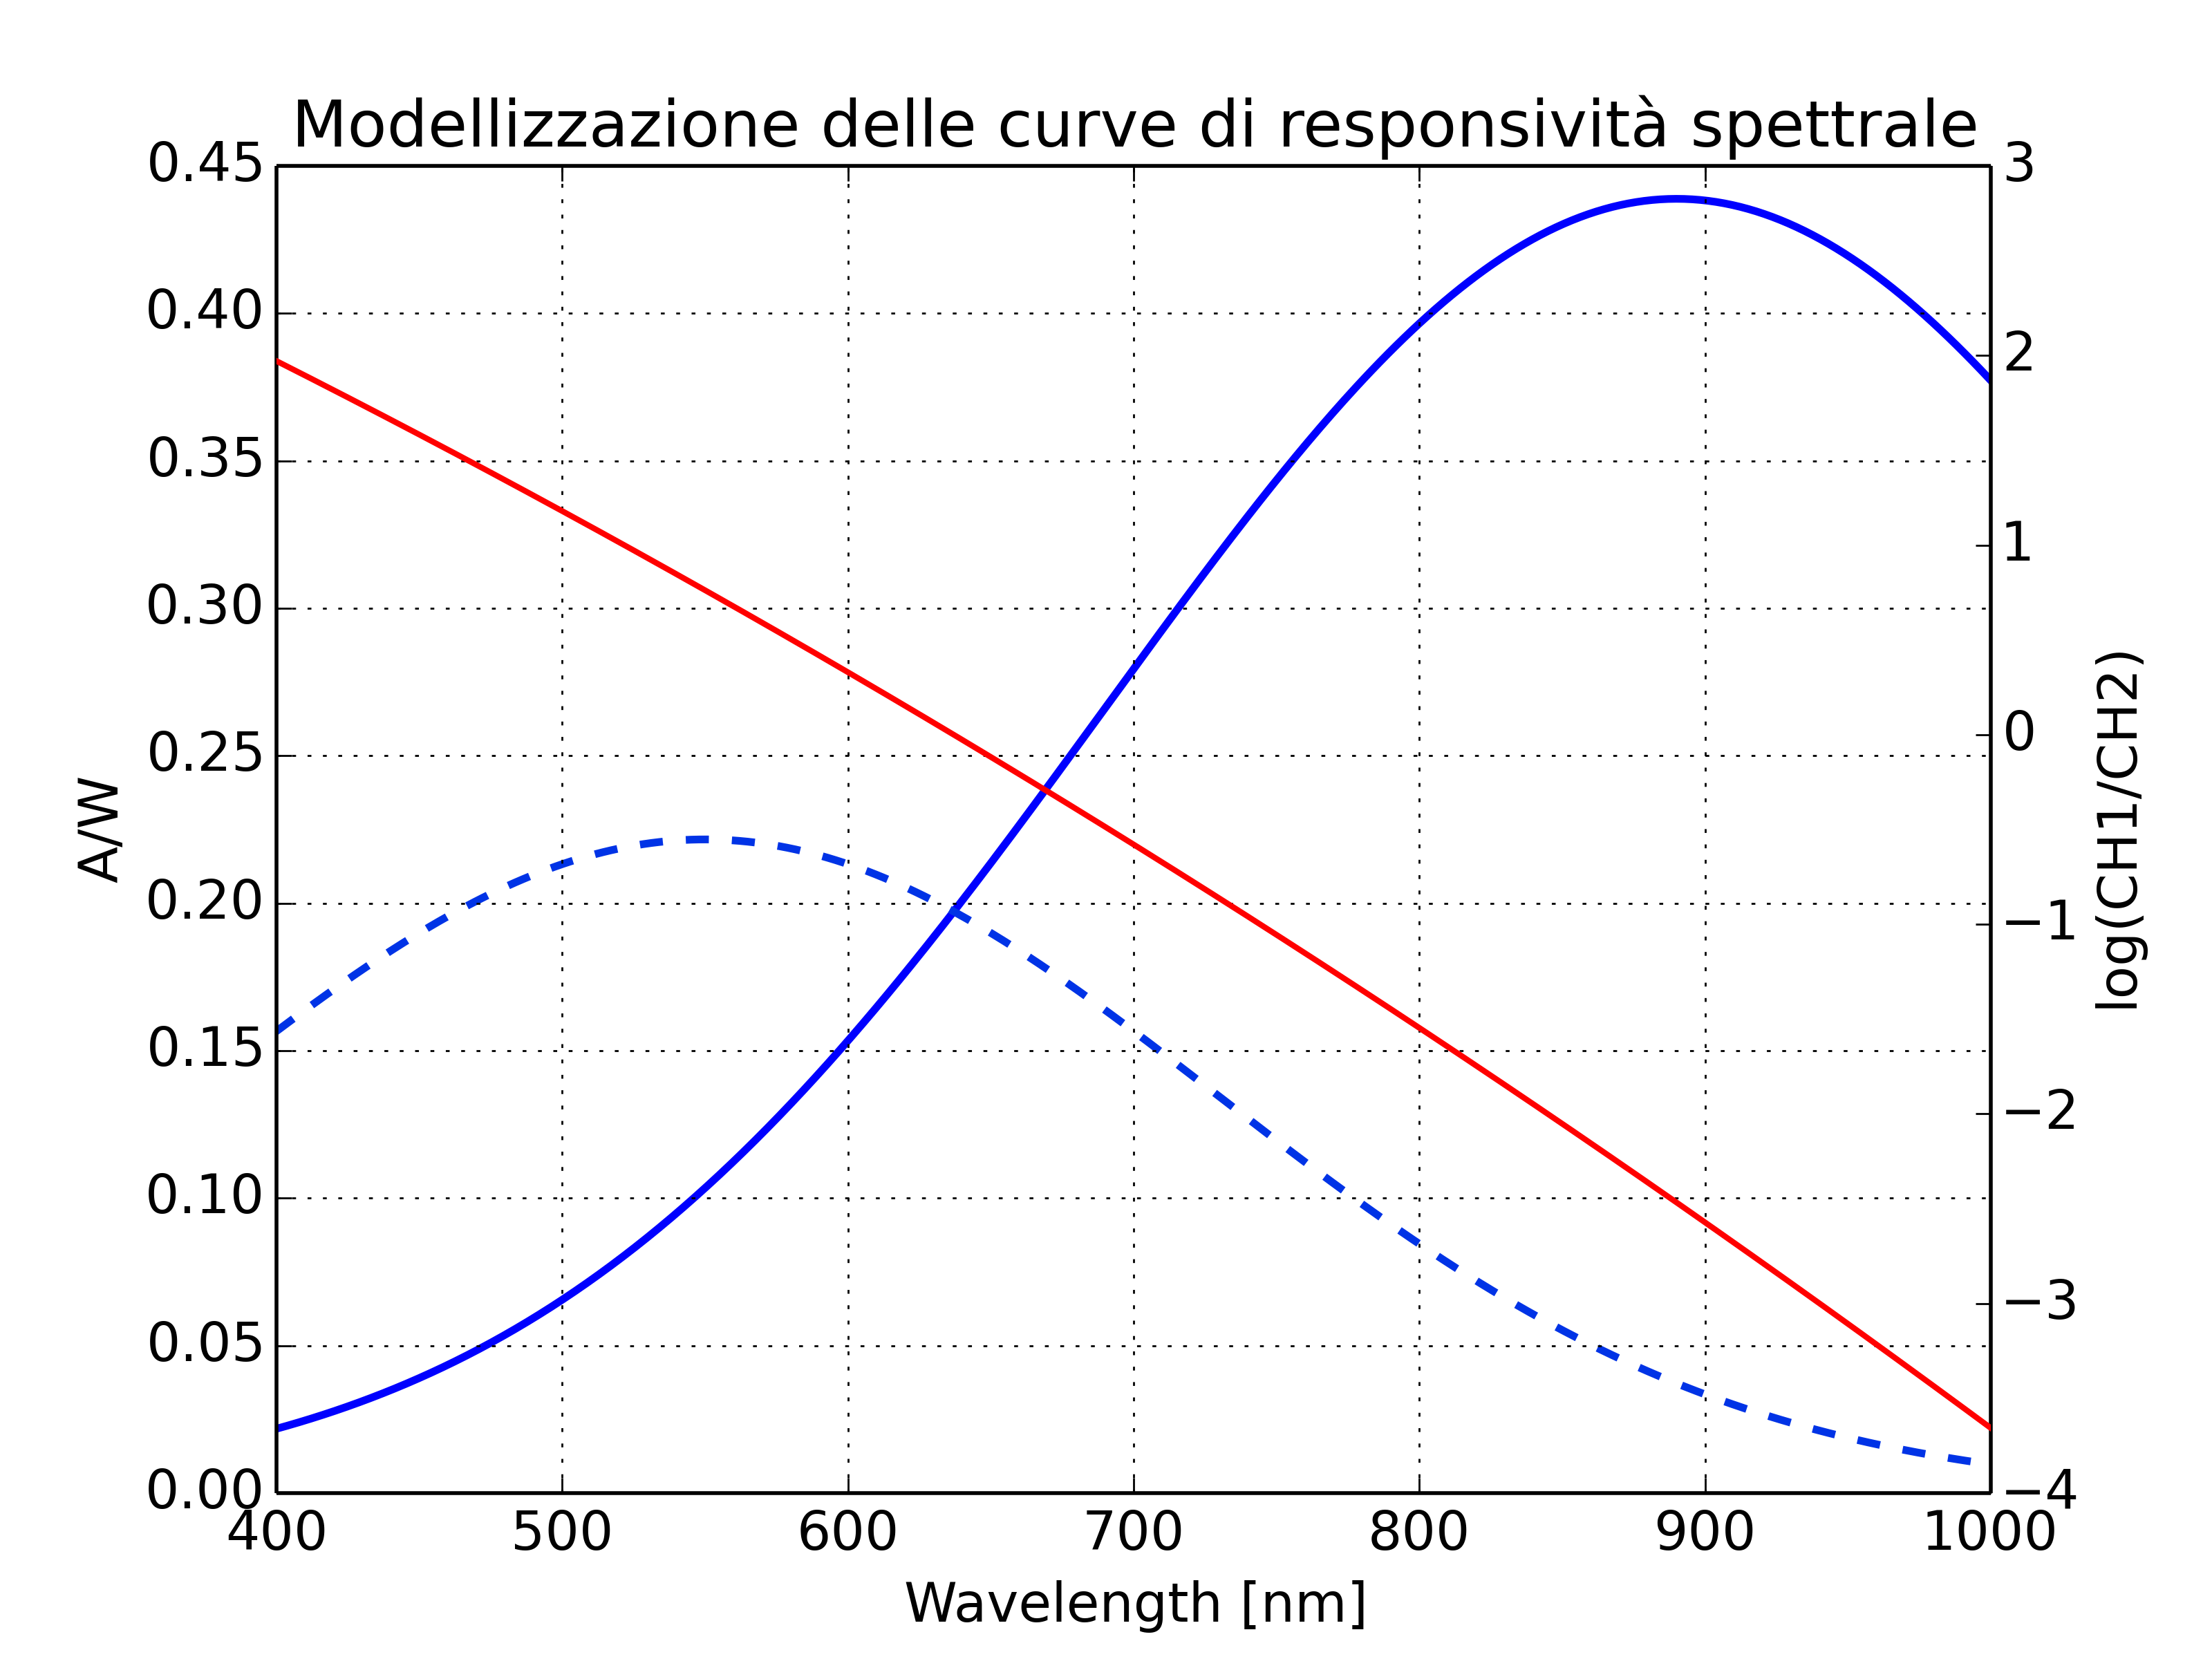
\includegraphics[width=0.4\linewidth]{./normal_respons}
\label{fig:normal_respons}}
\subfloat[Curva di responsività spettrale dei due diodi.]{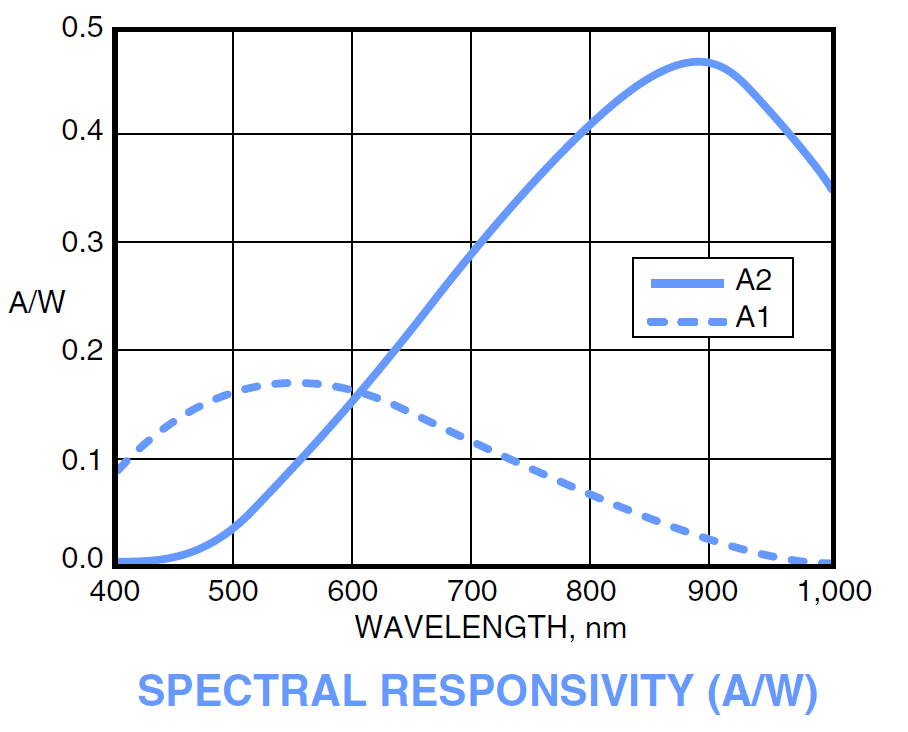
\includegraphics[width=0.4\linewidth]{./spectral_respo}
\label{fig:spectral_respo}}
\end{figure}


\end{frame}

\begin{frame}
Risultato:
\begin{figure}
\centering
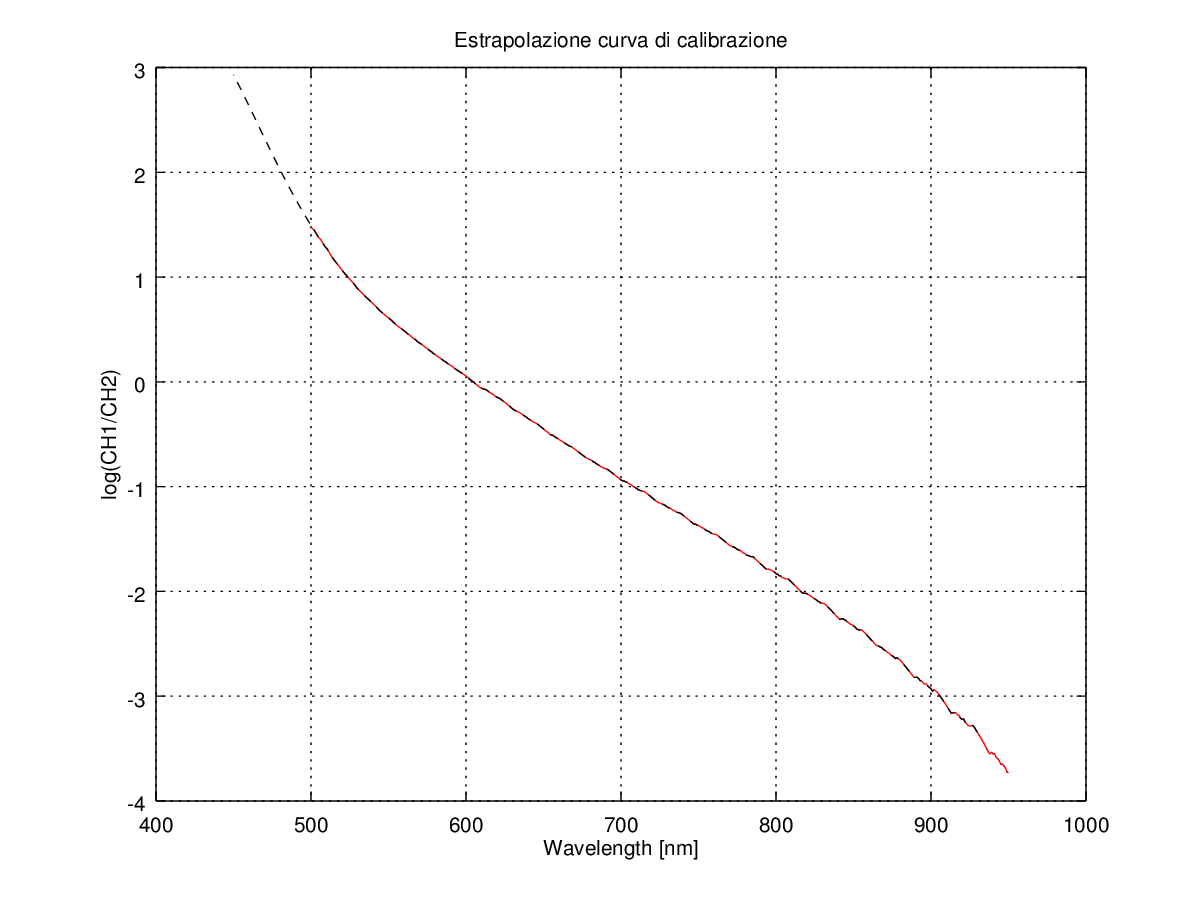
\includegraphics[width=0.7\linewidth]{./calibrazione_ext}
\caption{Curva di calibrazione "estesa" interpolata con un polinomio di grado 11.}
\label{fig:calibrazione_ext}
\end{figure}
\end{frame}


\begin{frame}{Caratterizzazione dei LED - II}

\begin{figure}
\centering
\subfloat[Dispersione dei LED sulla curva di calibrazione 'estesa'.]{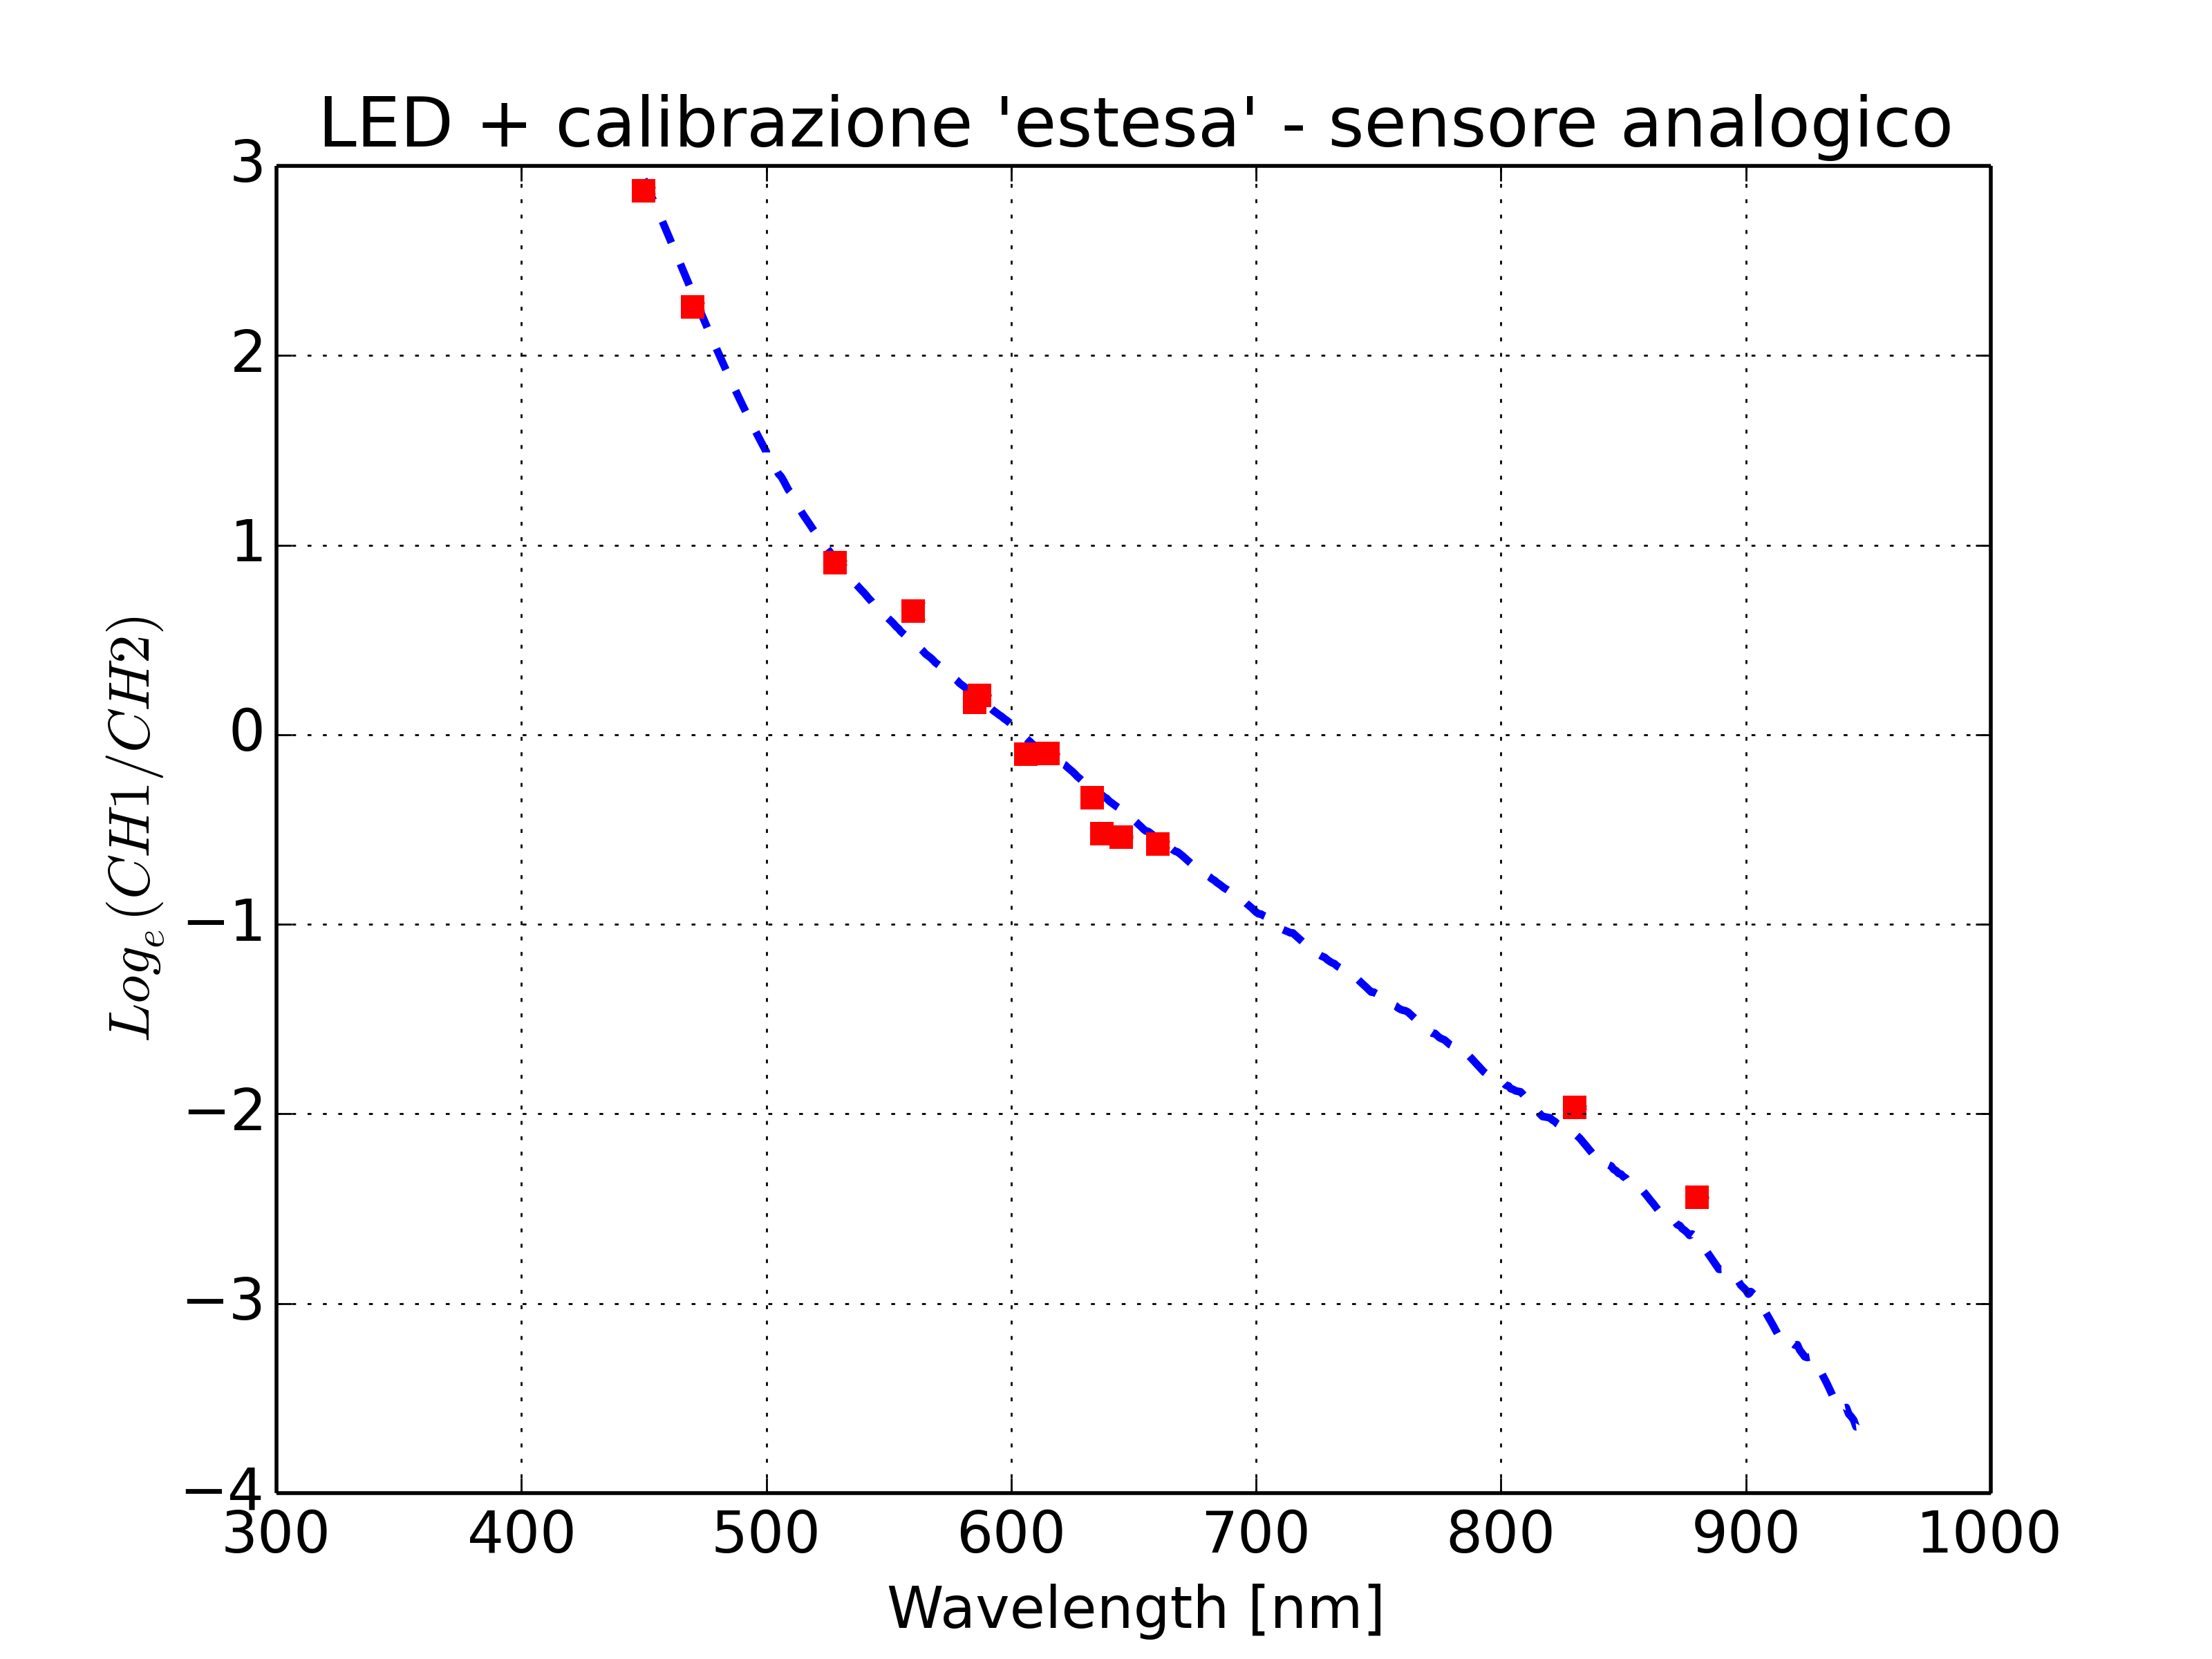
\includegraphics[width=0.55\linewidth]{./calibrazione_LED_extended}
\label{fig:calibrazione_LED_extended}}
\subfloat[Scarto fra lunghezze d'onda datasheet e da "calibrazione".]{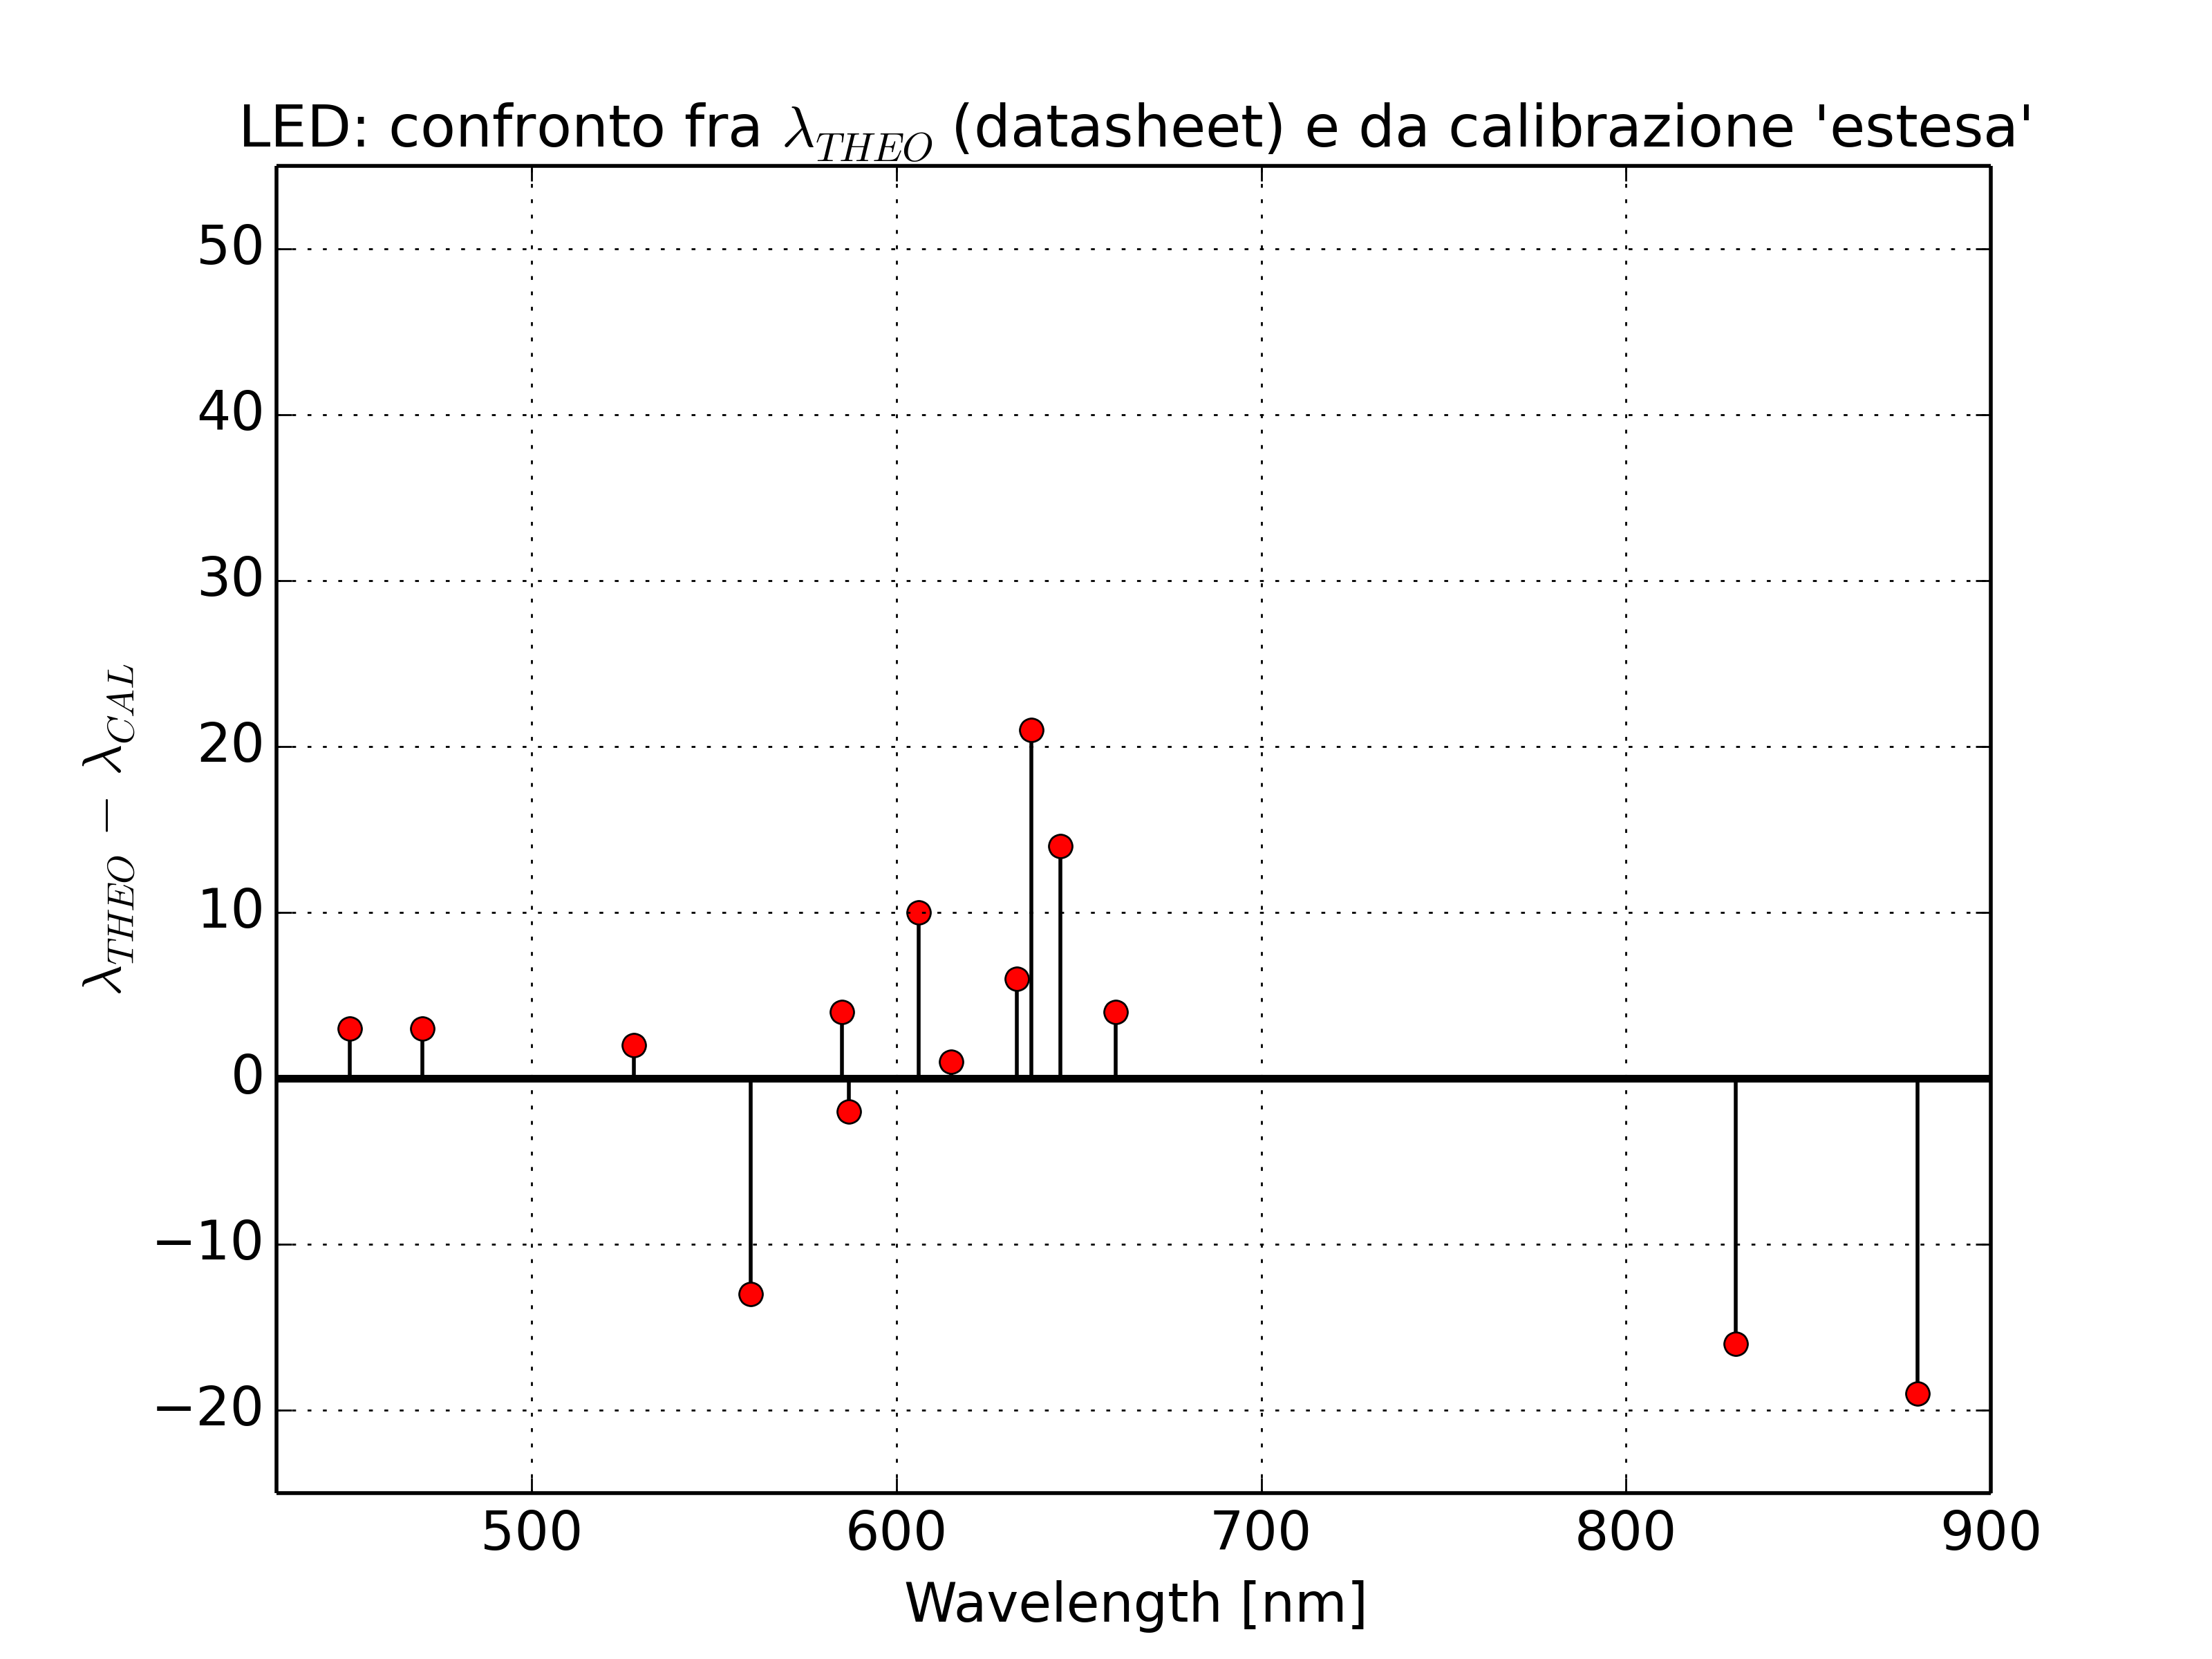
\includegraphics[width=0.55\linewidth]{./LED_confronto_extended}
\label{fig:LED_confronto_extended}}
\end{figure}
\end{frame}


\begin{frame}
\begin{table}[h]
\centering
% This LaTeX table template is generated by emacs 24.3.1
\begin{tabular}{l|c|c}
\hline
\textbf{LED} & $\lambda$ nom. [nm] & $\lambda$ calibr. [nm] \\
\hline
\textsc{hlmpd101-645} & 645 & 659(1) \\
\textsc{hlmpc115-red} & 637 & 658(2)  \\
\textsc{hlmpc315-Y} & 585 & 589(2)  \\
\textsc{la3366} & 615 & 616(1) \\
\textsc{lb3333} & 470 & 473(1) \\
\textsc{led450} & 450 & 453(1) \\
\textsc{lo3336} & 606 & 616(1) \\
\textsc{lpk376} & 560 & 547(4) \\
\textsc{ls3336} & 633 & 639(1) \\
\textsc{lt3333} & 528 & 530(1) \\
\textsc{ly3336} & 587 & 585(1) \\
\textsc{sfh4873-880} & 880 & 861(1) \\
\textsc{ssl-lxa} & 660 & 664(2) \\
\textsc{tshg8400-830} & 830 & 814(1) \\
\hline
\end{tabular}
%\caption{Lunghezze d'onda dei LED ricavate da calibrazione del sensore analogico.}
%\label{tabella_LED_ext}
\end{table}
\end{frame}

\section{Applicazione: lunghezze d'onda e triplette RGB}
\subsection{Prova APDS-9301}

\begin{frame}{Colori RGB}
\begin{itemize}
\item È stato impiegato un programma di OCTAVE che mostra una finestra di colore variabile secondo una matrice di 300 triplette RGB\\
\item Prima e dopo la fine della serie di colori è stato posto un fondo nero (0,0,0) come riferimento\\
\item Per ogni punto è stata ricavata l'intensità e la lunghezza d'onda tramite la curva di calibrazione.
\end{itemize}
\end{frame}

\begin{frame}{Colori RGB: sequenza triplette}
\centering
\begin{figure}
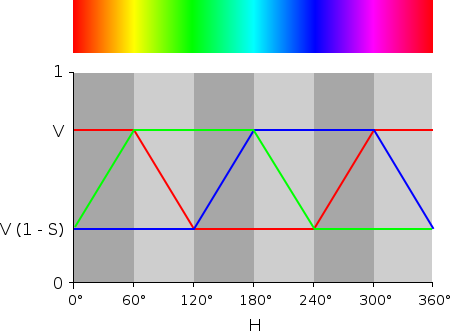
\includegraphics[scale=.5]{sequence}
\end{figure}
\end{frame}

\begin{frame}{Colori RGB: misure e confronto}
\begin{textblock}{12}(-2,3.2)
\begin{figure}
\centering
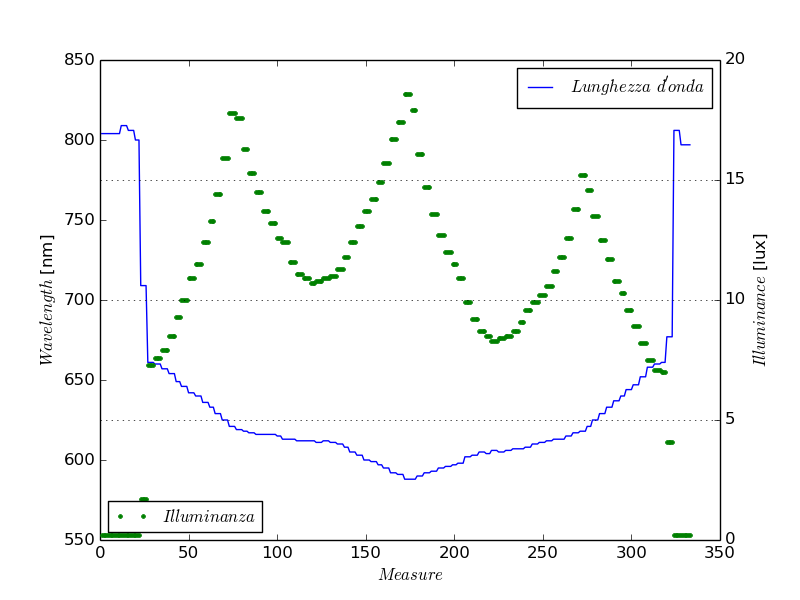
\includegraphics[width=0.6\linewidth]{./comparison}
\caption{Dati APDS-9301}
\label{fig:resp}
\end{figure}
\end{textblock}


\begin{textblock}{12}(6,3.2)
\begin{figure}
\centering
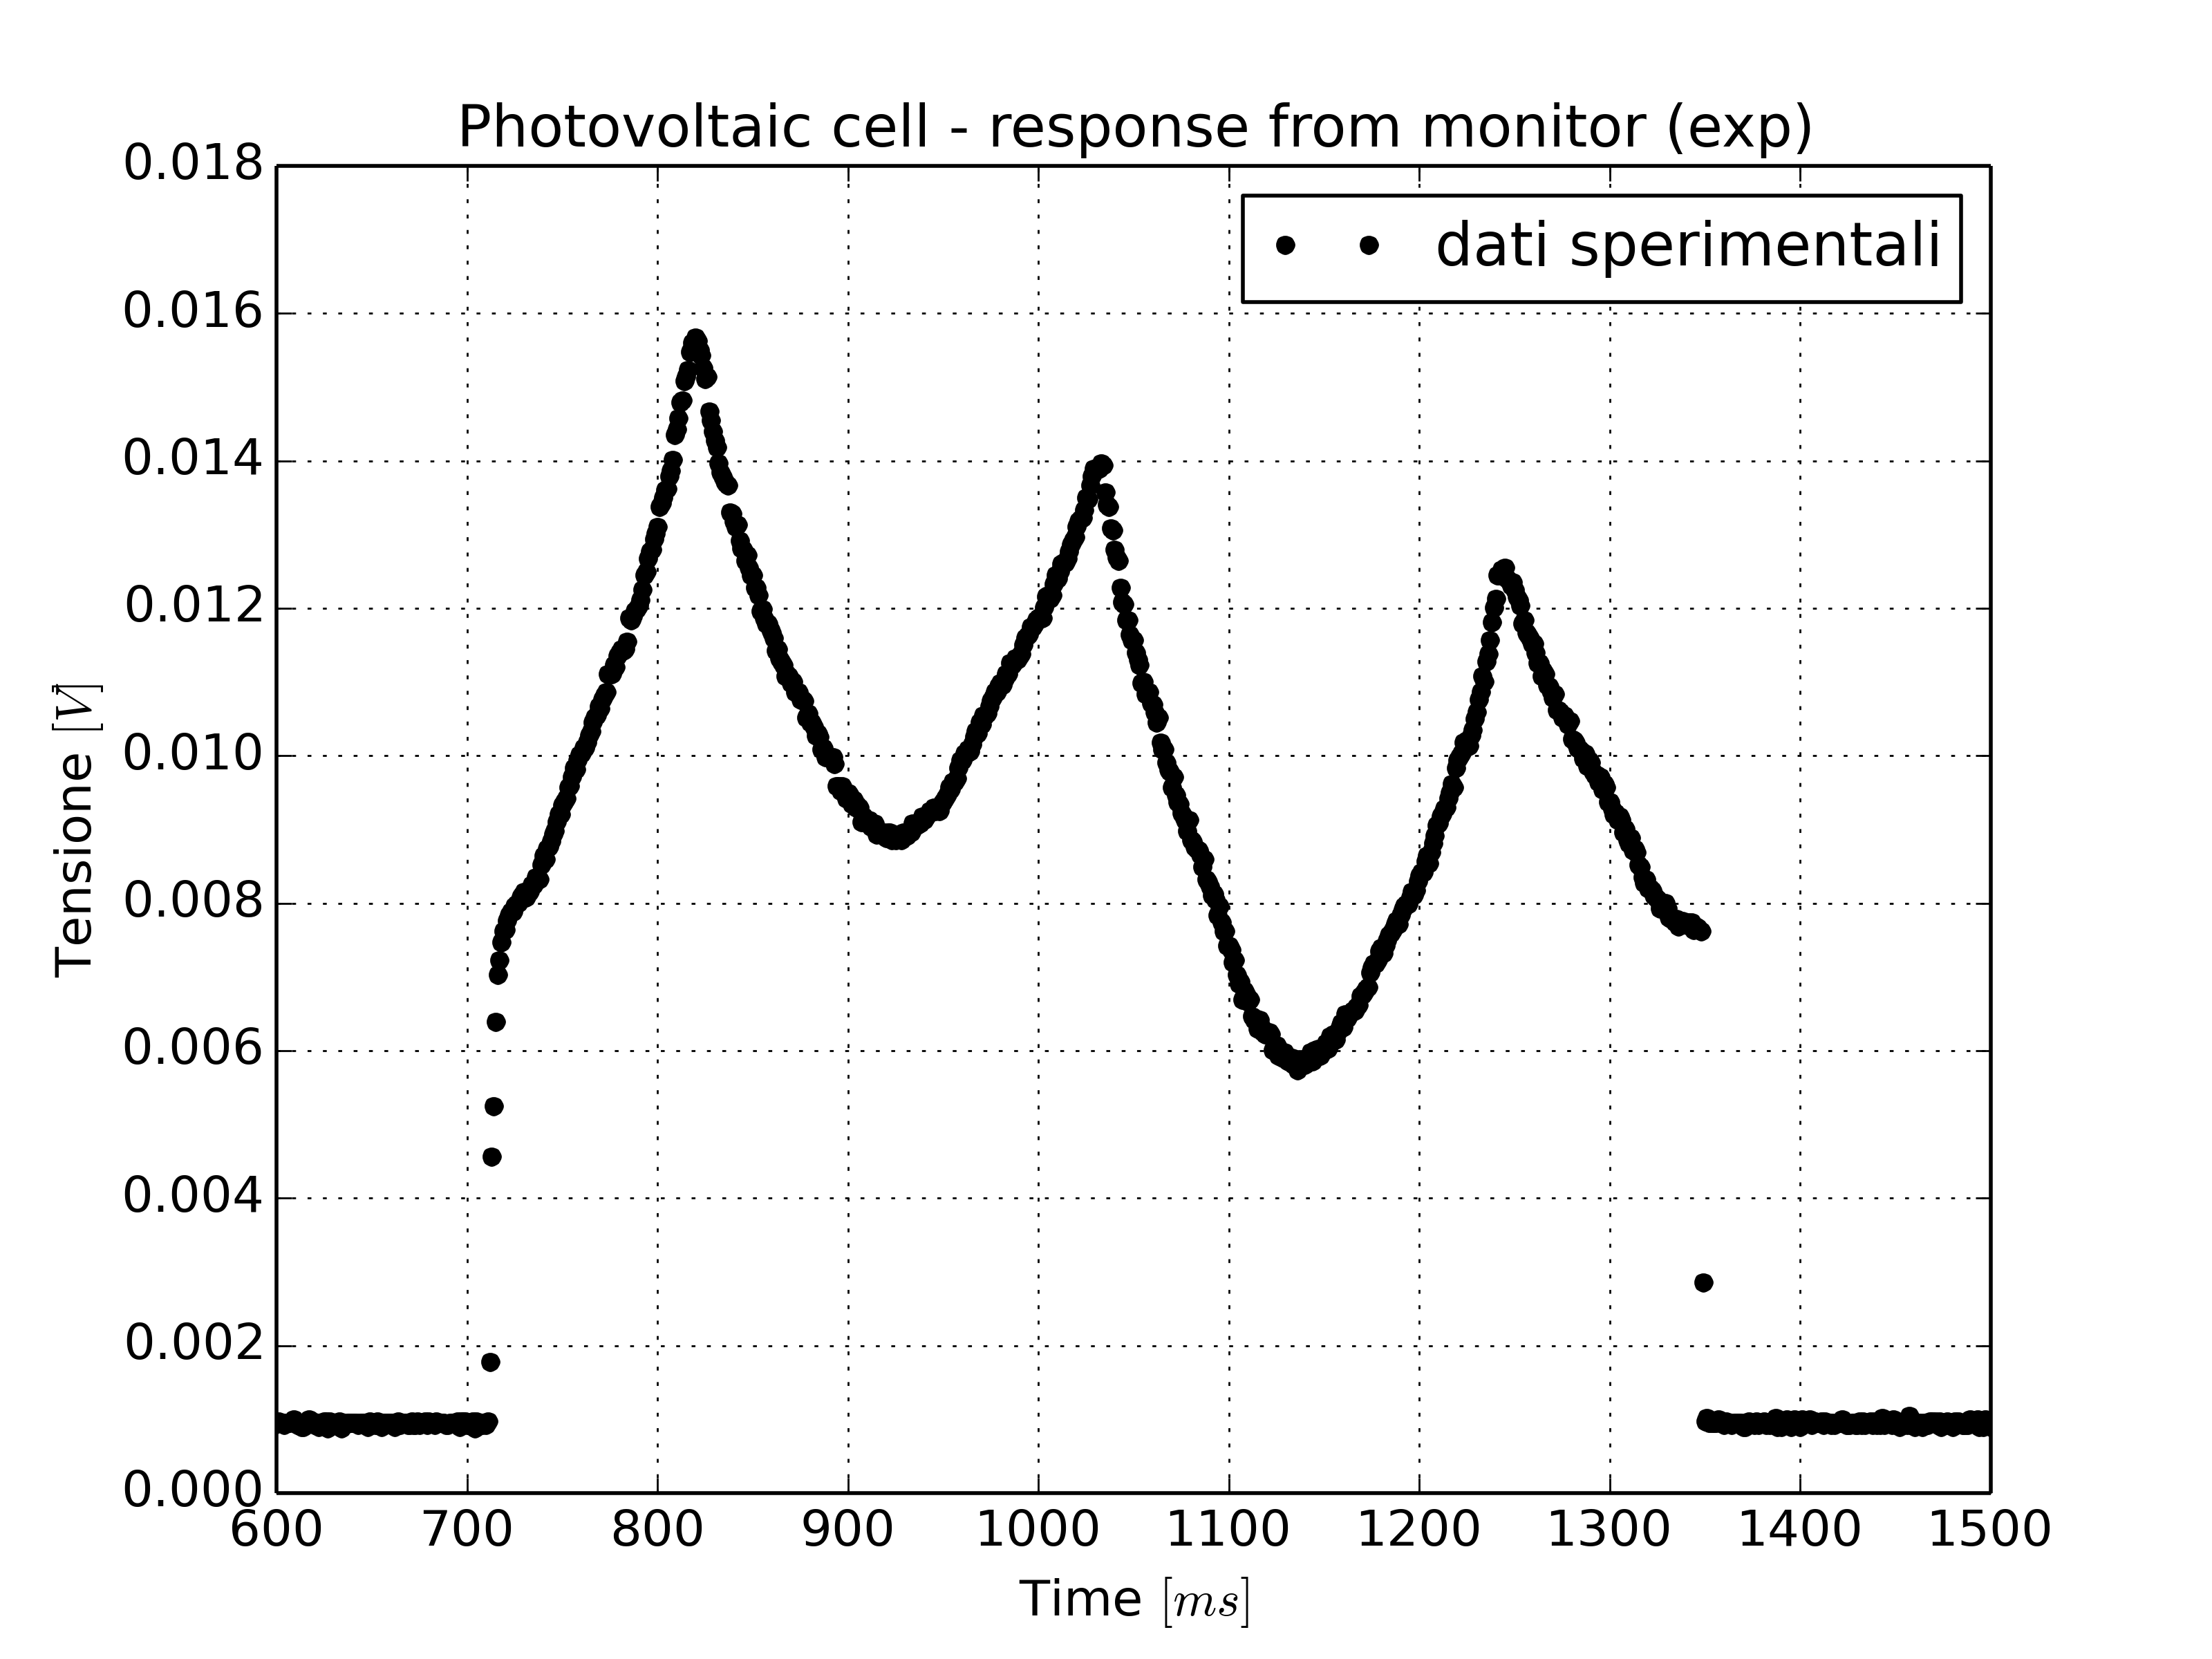
\includegraphics[width=0.6\linewidth]{./1_dati_sperimentali}
\caption{Dati cella fotovoltaica}
\label{fig:cal}
\end{figure}
\end{textblock}
\end{frame}

\begin{frame}{Colori RGB: osservazioni}
\begin{itemize}
\item Curve di illuminazione molto simili;\\
\item In generale lunghezze d'onda molto diverse
\item Minima lunghezza d'onda $\approx$ 580 nm (giallo), neanche in corrispondenza del blu (secondo minimo);\\
\item Illuminazione non nulla per il nero, ma si rileva luce a 800 nm circa (infrarosso).
\end{itemize}
\end{frame}

\begin{frame}{WARNING}
NON possiamo parlare di lunghezze d'onda per i colori ottenuti come somma di R,G,B.\\
Definizione valida SOLO per i colori puri.
\end{frame}

\begin{frame}{Colori RGB: possibile soluzione}
\begin{itemize}
\item Fondo infrarosso non trascurabile;
\item Ipotesi: il fondo infrarosso rimane costante durante la presa dati;
\item I valori in uscita da CH0 e CH1 dati dalla somma dei valori che si avrebbero se sul rilevatore incidesse solo radiazione monocromatica della stessa frequenza e intensità di quelle che compongono quella che effettivamente viene rilevata;
\item Possibile soluzione: sottrarre a CH0 e CH1 il fondo infrarosso, in questo caso i valori a schermo nero, rispettivamente 62 e 37.
\end{itemize}
\end{frame}

\begin{frame}{Colori RGB: risultato}
\begin{textblock}{9}(2.6,3.0)\begin{figure}
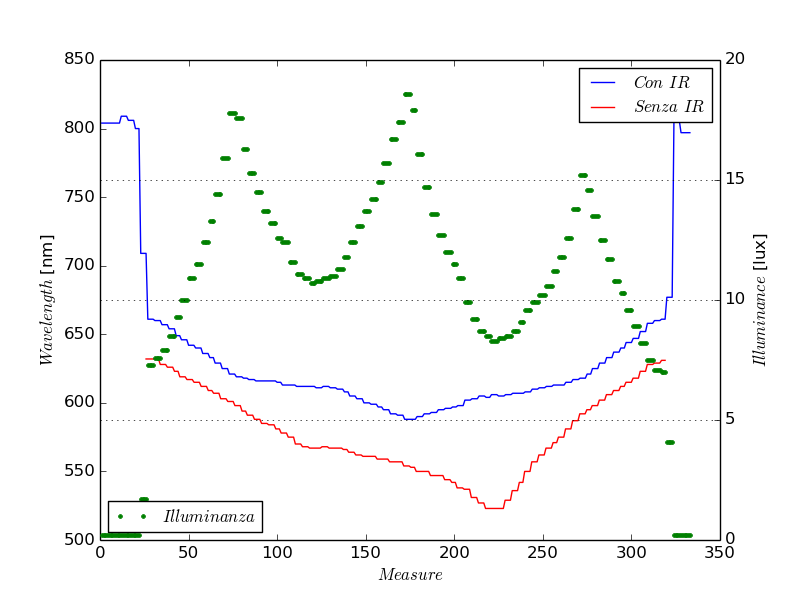
\includegraphics[scale=.42]{comparison3}
\end{figure}
\end{textblock}
\end{frame}

\begin{frame}{Colori RGB: conclusioni}
\begin{itemize}
\item Nuova curva ''sincronizzata'' con i minimi;\\
\item Divario maggiore nei minimi di illuminazione, minore nei massimi;\\
\item Lunghezze d'onda dei colori puri ancora poco precise, circa la stessa differenza che con i LED.
\end{itemize}
\end{frame}

\subsection{Colori RGB: WS-7.56-TO5}

\begin{frame}{Rilevazione del segnale}
\begin{figure}
\centering
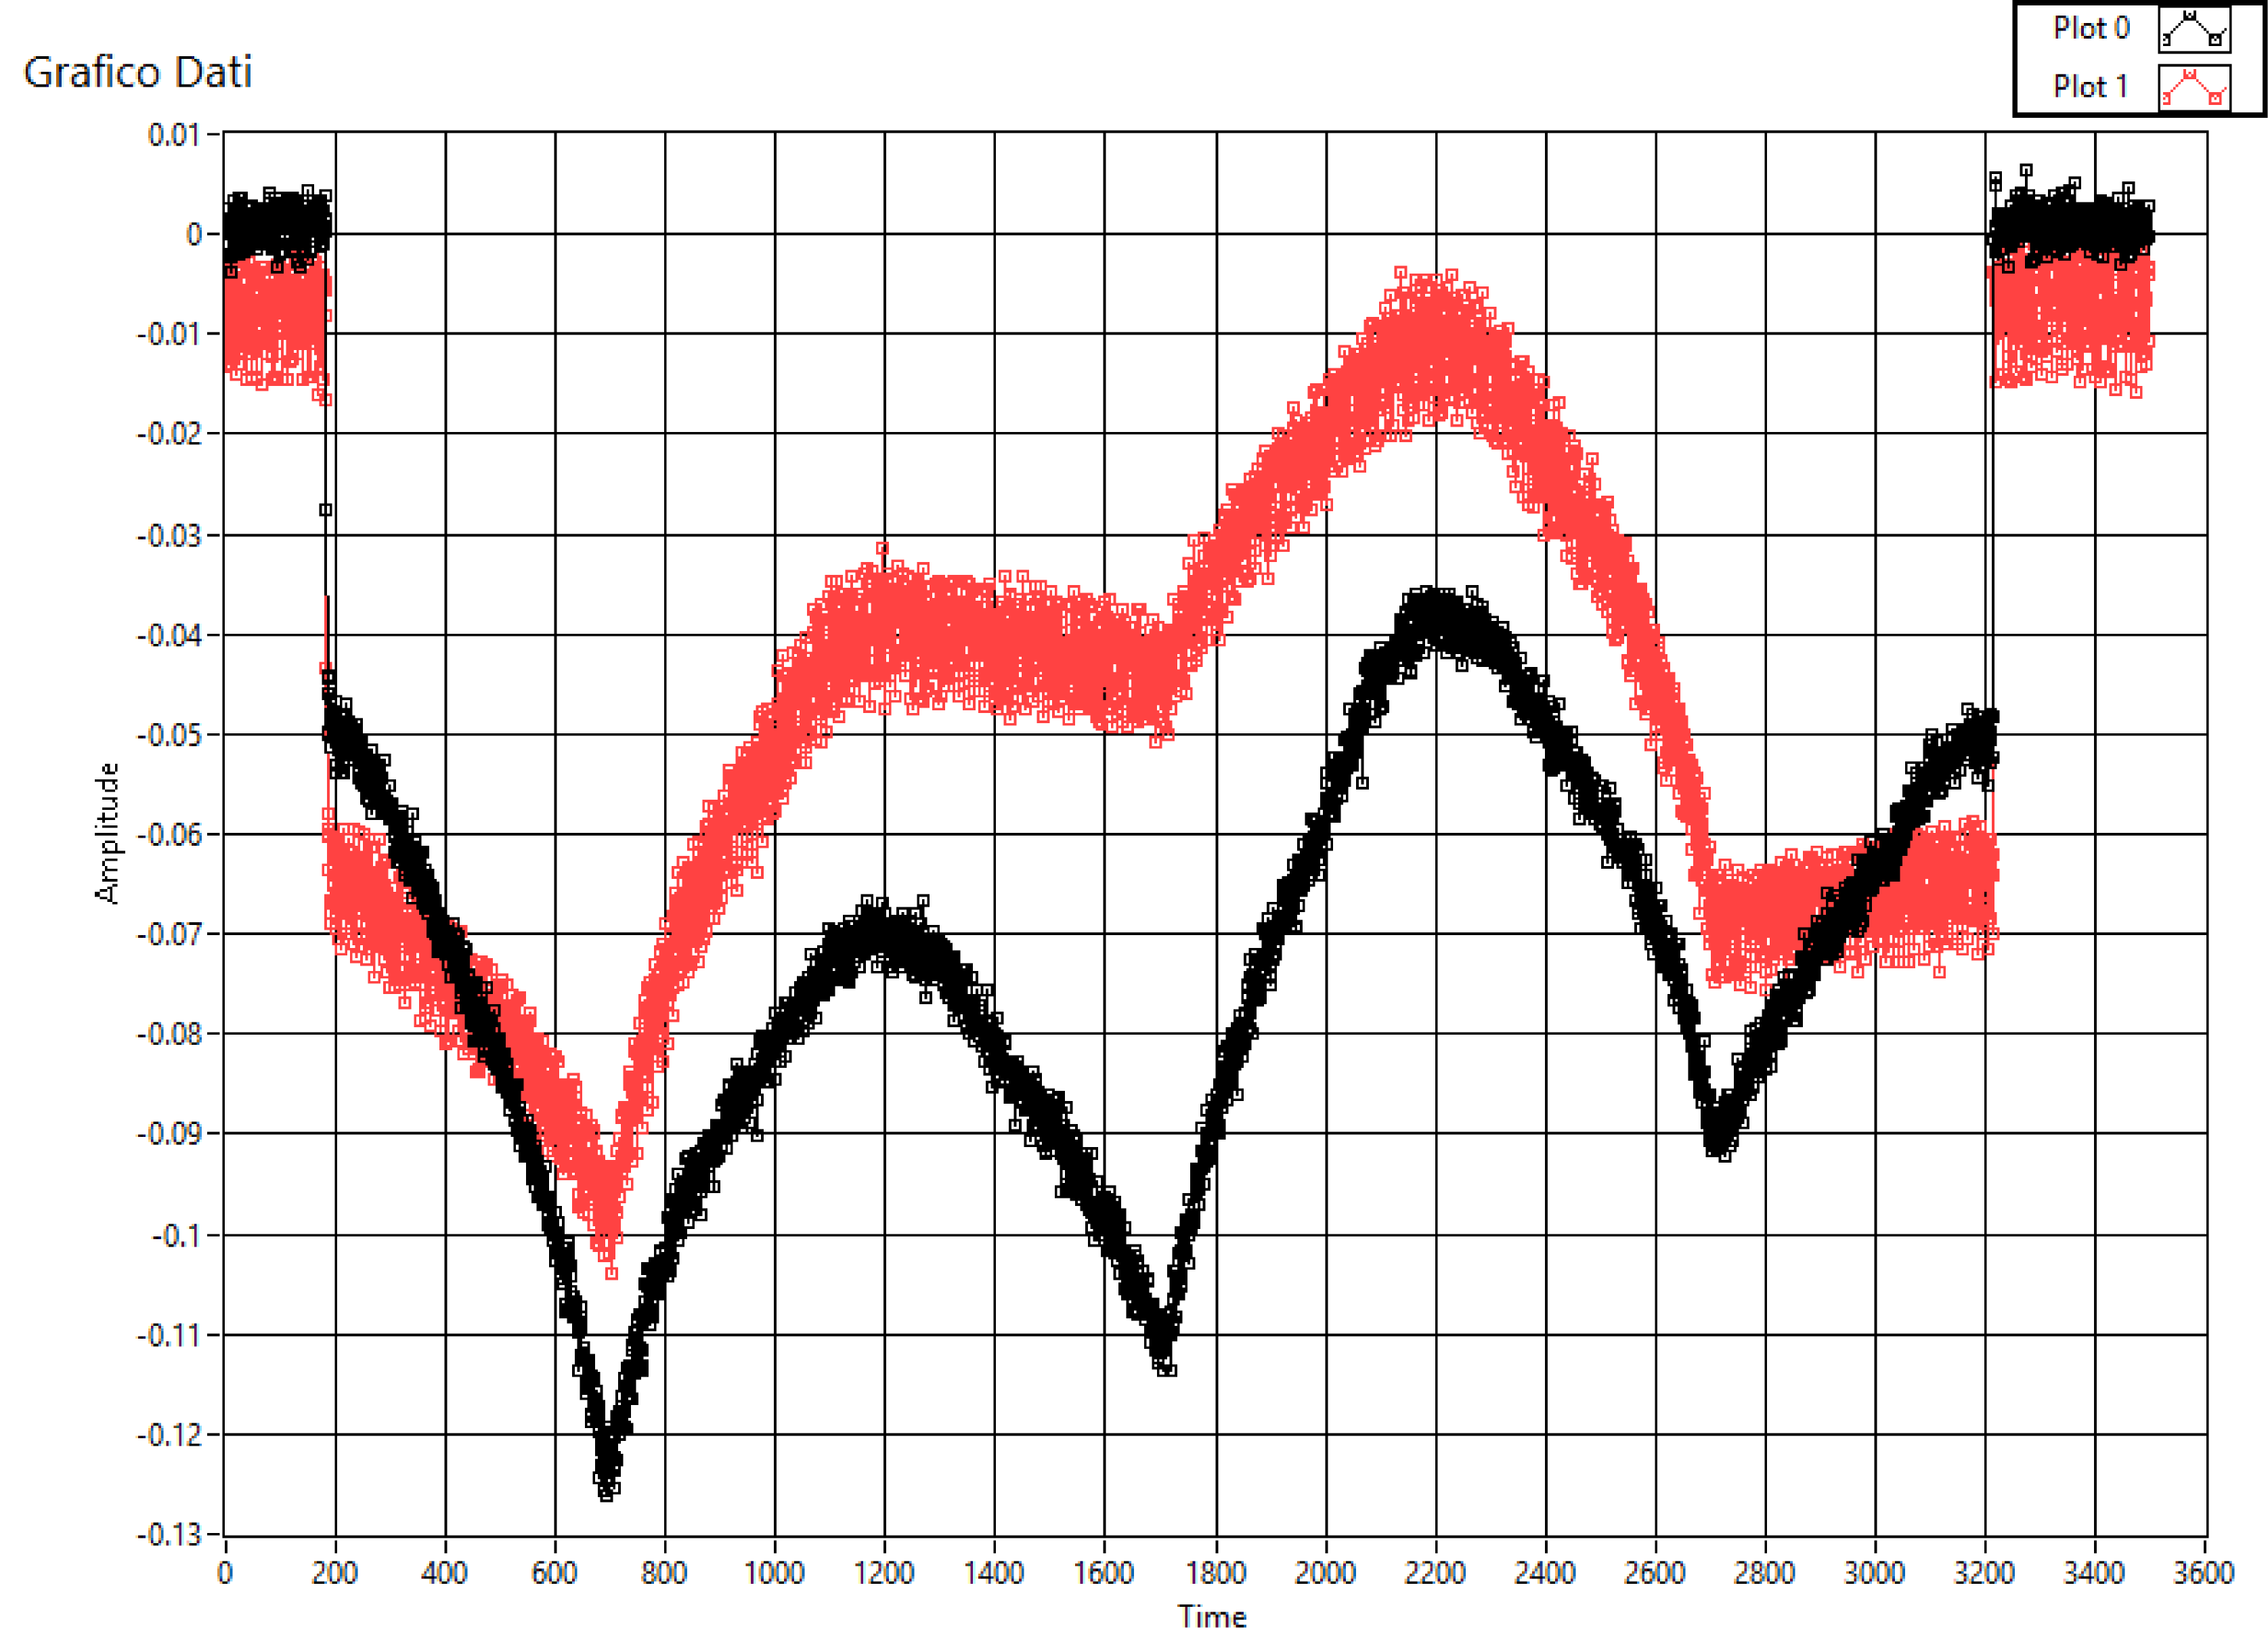
\includegraphics[width=0.4\linewidth]{./analog_monitor_colori}
%\caption{Segnali di tensione dei due canali CH1, CH2 durante lo svolgimento dello script.}
\label{fig:analog_monitor_colori}
\end{figure}

\fontsize{9}{11}
\begin{itemize}
\item 300 triplette RGB intervallate l'una dall'altra da 0.1s
\item I picchi negativi corrispondono alle situazioni RGB del tipo (110, 101, 011).
\item Le \textit{valli} (immaginando ribaltata l'immagine) sono invece le triplette pure (100, 010, 001).
\item Il segnale del CH2 (in rosso) nel grafico, ha una risposta molto marcata sul rosso (colore), come ci aspettiamo dalla responsività spettrale.
\end{itemize}
\end{frame}

\begin{frame}{Segnale pulito}
\fontsize{9}{11}
\begin{itemize}
\item Alta rumorosità: microspostamenti del sensore avvenuti durante l'acquisizione $\rightarrow$ interferenze da parte della luce ambientale
\item Alta rumorosità: distorsione cromatica dovuta pressione su delle porzioni di monitor LCD, potrebbe aver reso il colore disomogeneo.
\end{itemize}
\begin{figure}
\centering
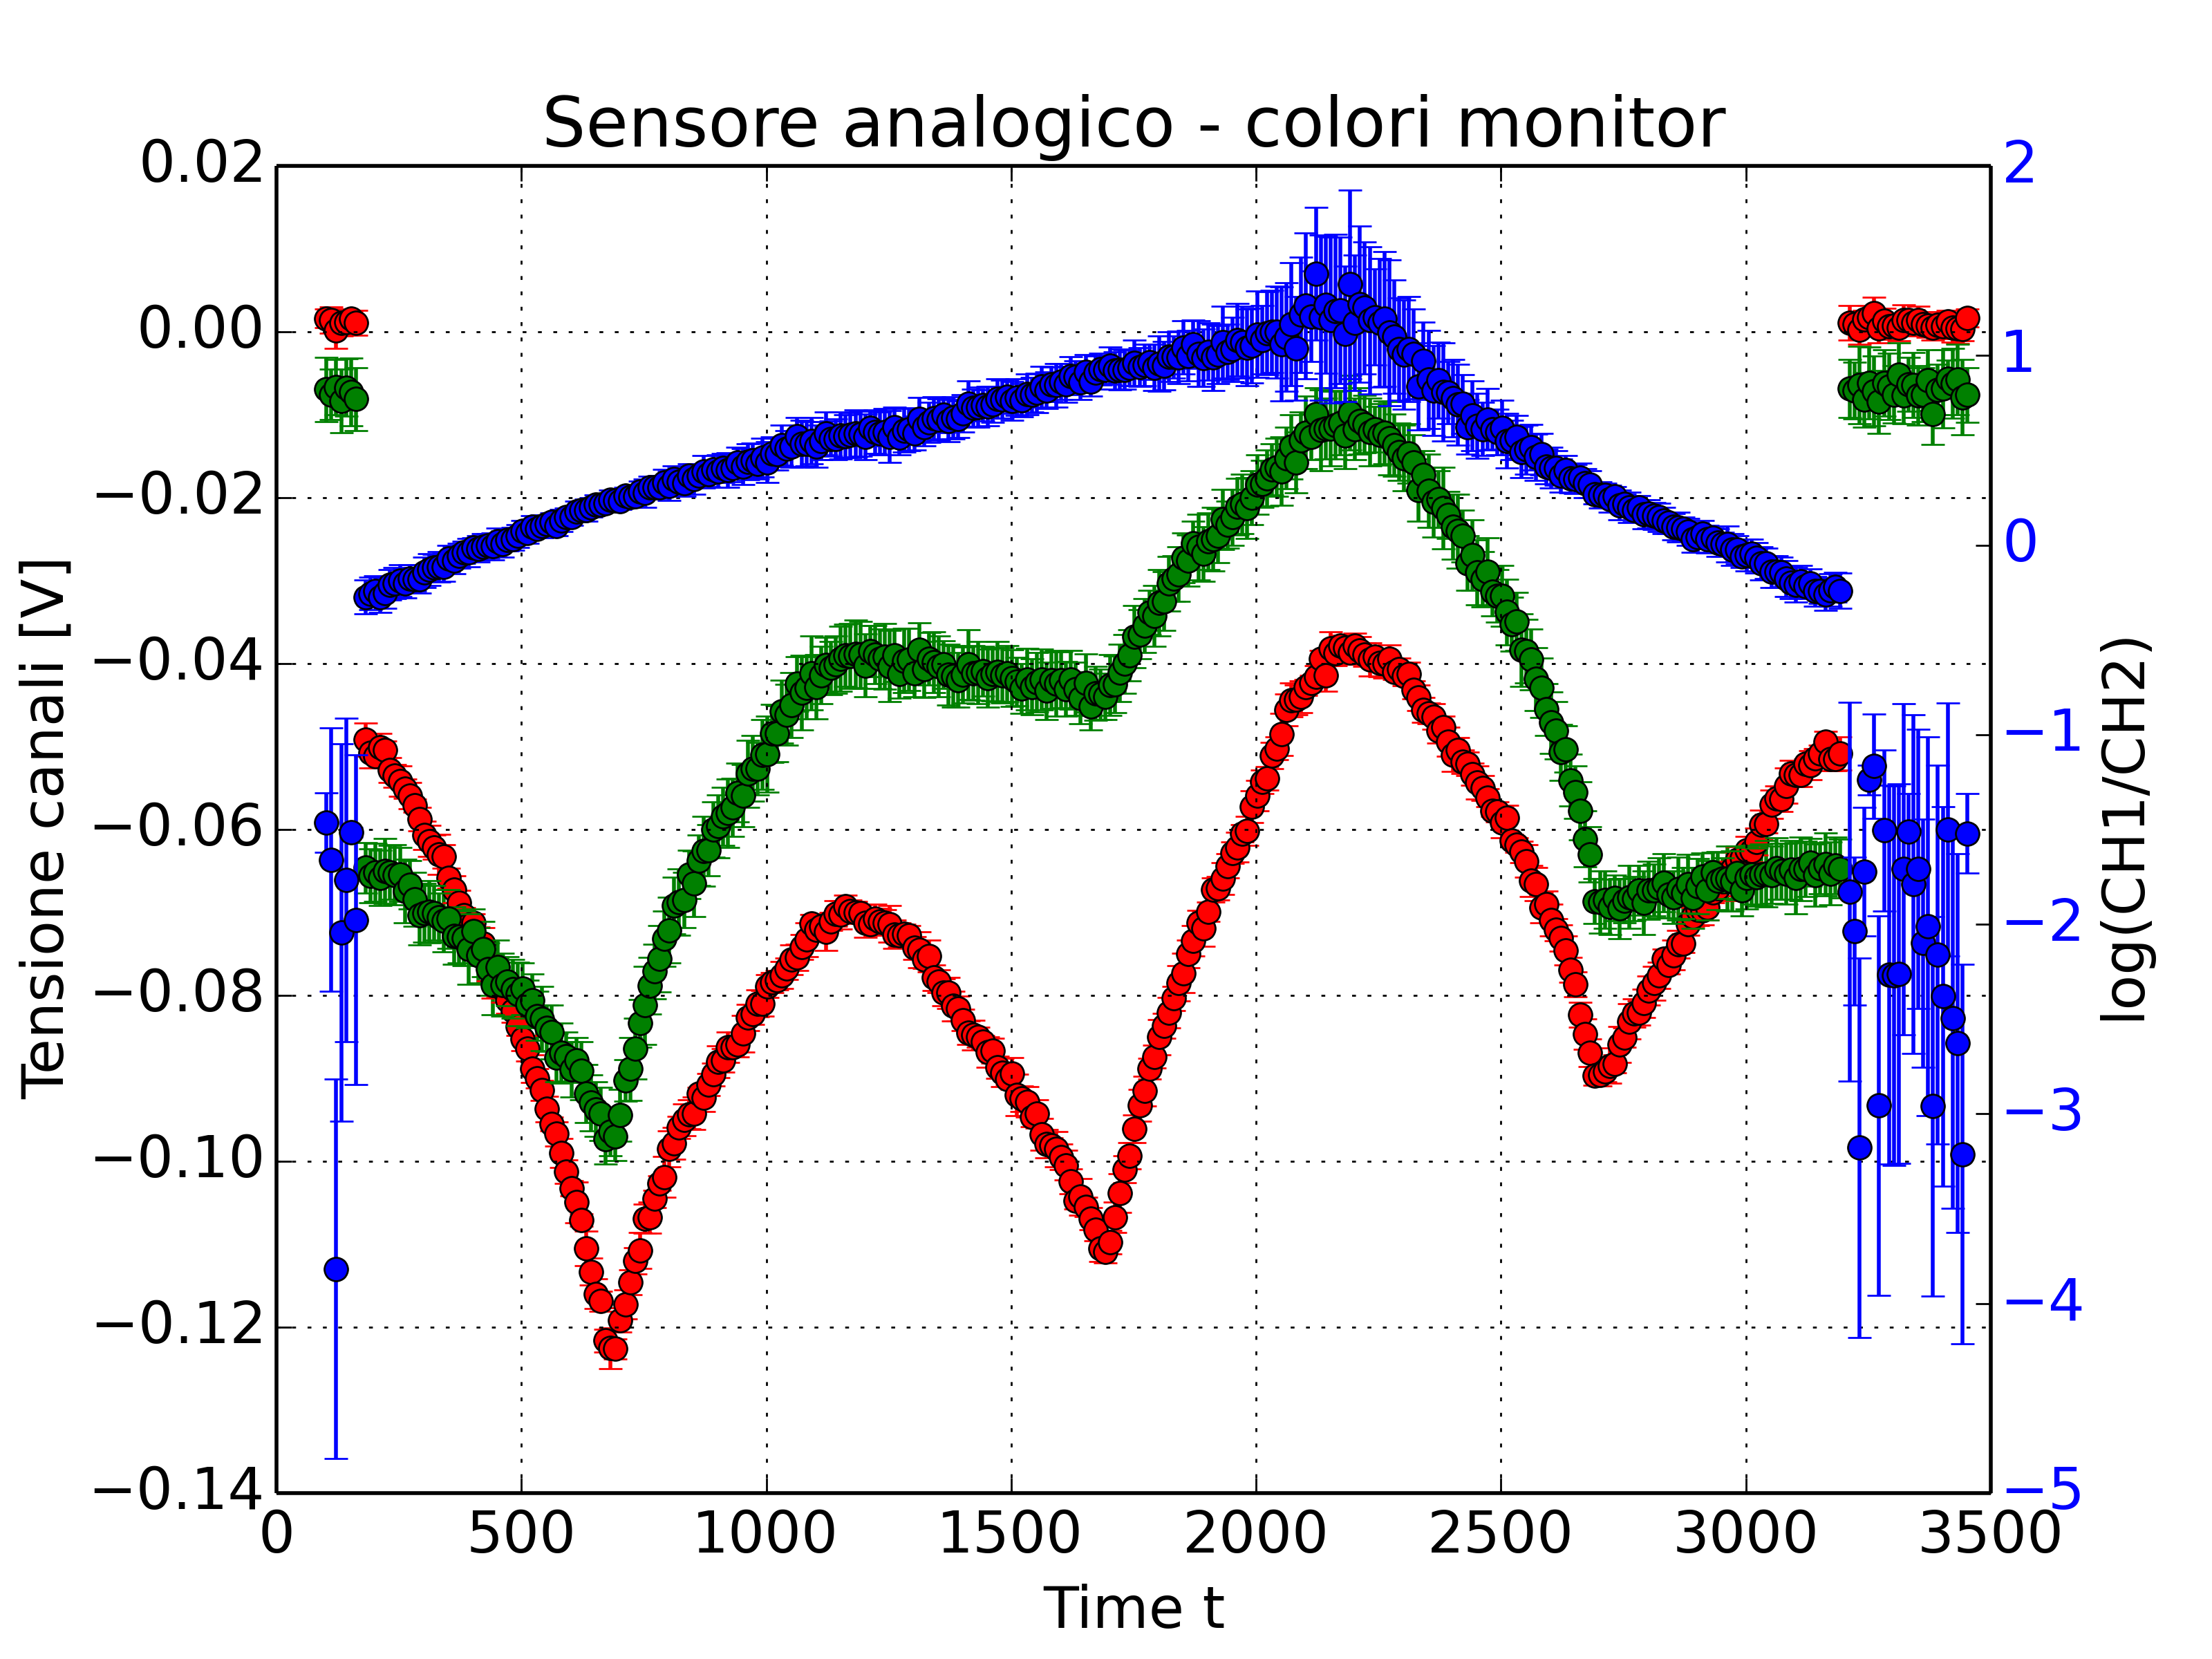
\includegraphics[width=0.6\linewidth]{./analog_segnale_log_average}
%\caption{Segnale acquisito dal sensore mediato e ripulito, e logaritmo del rapporto.}
\label{fig:analog_segnale_log_average}
\end{figure}
\end{frame}

\begin{frame}
\begin{figure}
\centering
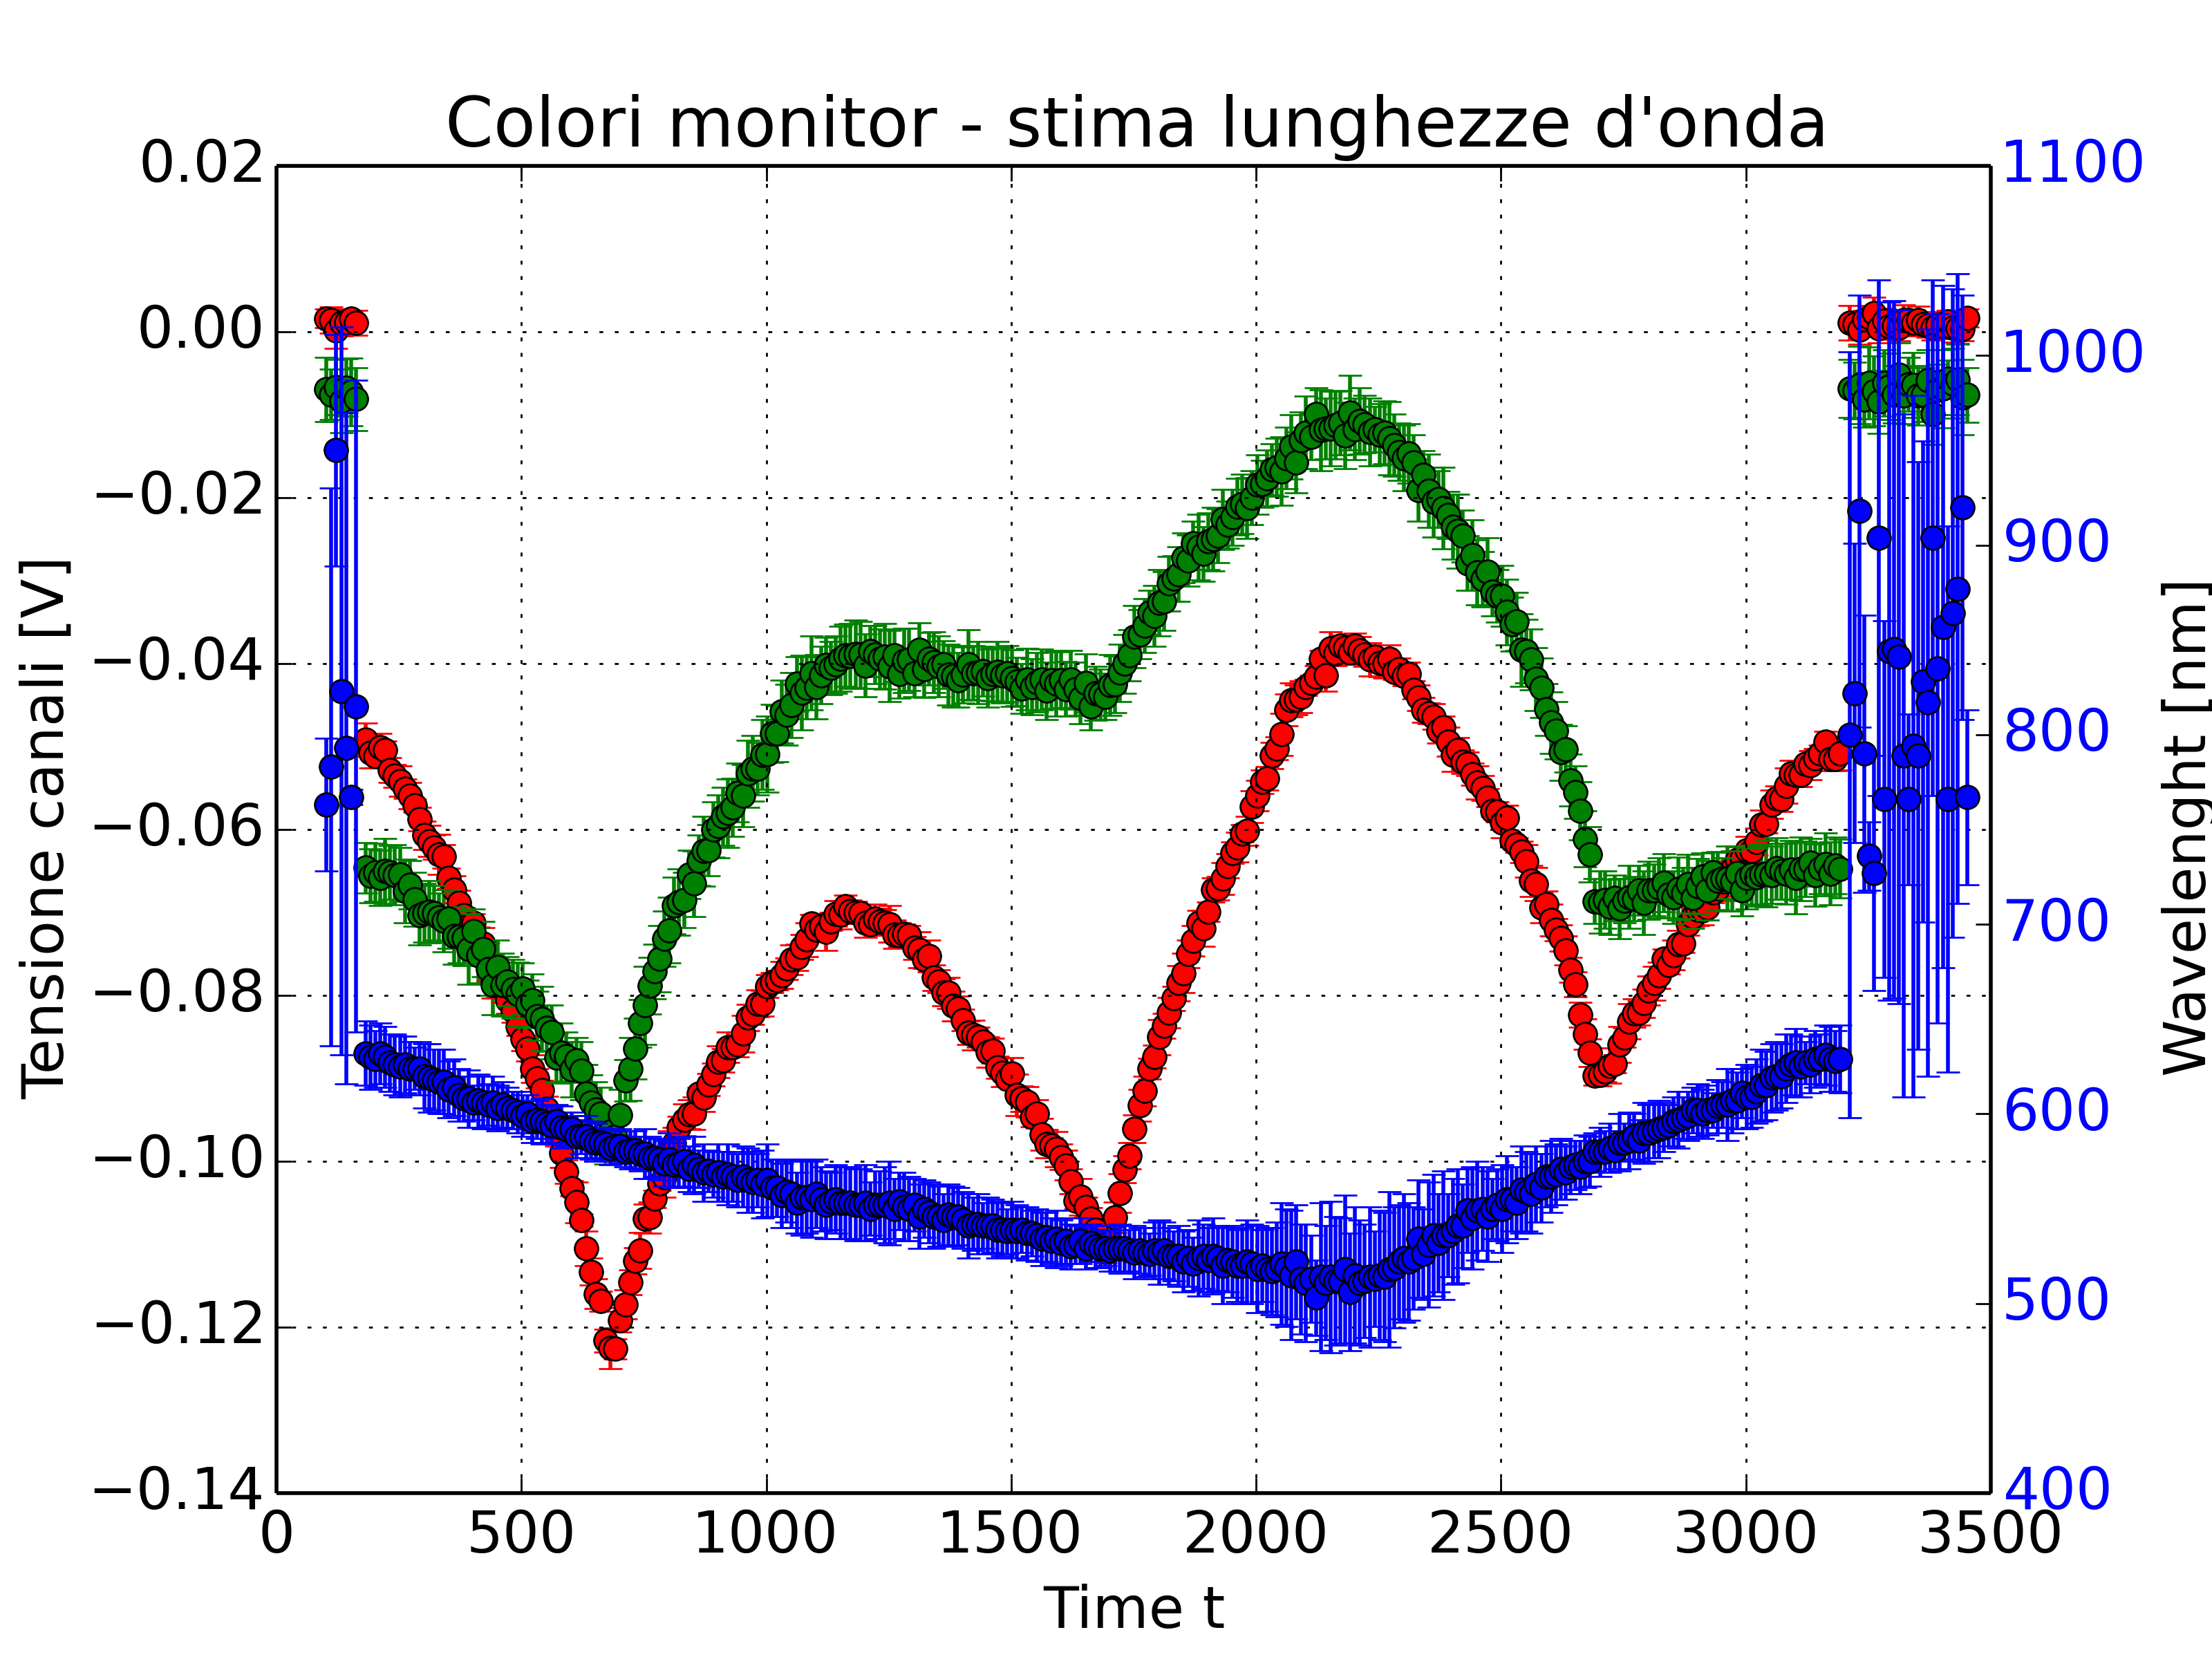
\includegraphics[width=0.6\linewidth]{./monitor_stima_lunghezzaonda}
%\caption{Stima della lunghezza d'onda a partire dal logaritmo del rapporto dei segnali, per ogni colore visualizzato sullo schermo.}
\label{fig:monitor_stima_lunghezzaonda}
\end{figure}

\begin{table}[h]
\centering
\begin{tabular}{c|c|c|c}
  & \textbf{RED} & \textbf{GREEN} & \textbf{BLUE} \\ 
 \hline Wavelength (nm) & 632(17) & 552(18) & 503(20) \\
 Colour ranges (nm) & 620-750 & 495-570 & 450-495 \\ 
\hline 
\end{tabular} 
\caption{Lunghezza d'onda dei colori puri RGB}
\label{RGB_lambda}
\end{table}
\end{frame}

\begin{frame}{Prime osservazioni}
\begin{itemize}
\item Gli intervalli in nm in cui vengono definiti i colori sono tratti da \textit{Thomas J. Bruno, Paris D. N. Svoronos. CRC Handbook of Fundamental Spectroscopic Correlation Charts}.
\item Il rosso riusciamo a stimarlo bene, il verde tende al giallo, il blu è accettabile solo entro i limiti dell'errore.
\item Segnale non nullo in corrispondenza del colore nero proiettato sul monitor LCD. Fenomeno è asimmetrico rispetto ai due fotodiodi: il diodo CH2, con curva di responsività piccata sul rosso rileva un segnale non trascurabile, contrariamente al diodo del CH1 che mostra tensioni compatibili con zero.
\item Nel caso del CH1 i due contributi del segnale di buio e IR si annullano a vicenda (uno è negativo e il secondo positivo).
\item Togliamo il fondo IR da CH2.
\end{itemize}
\end{frame}



\begin{frame}
\begin{figure}
\centering
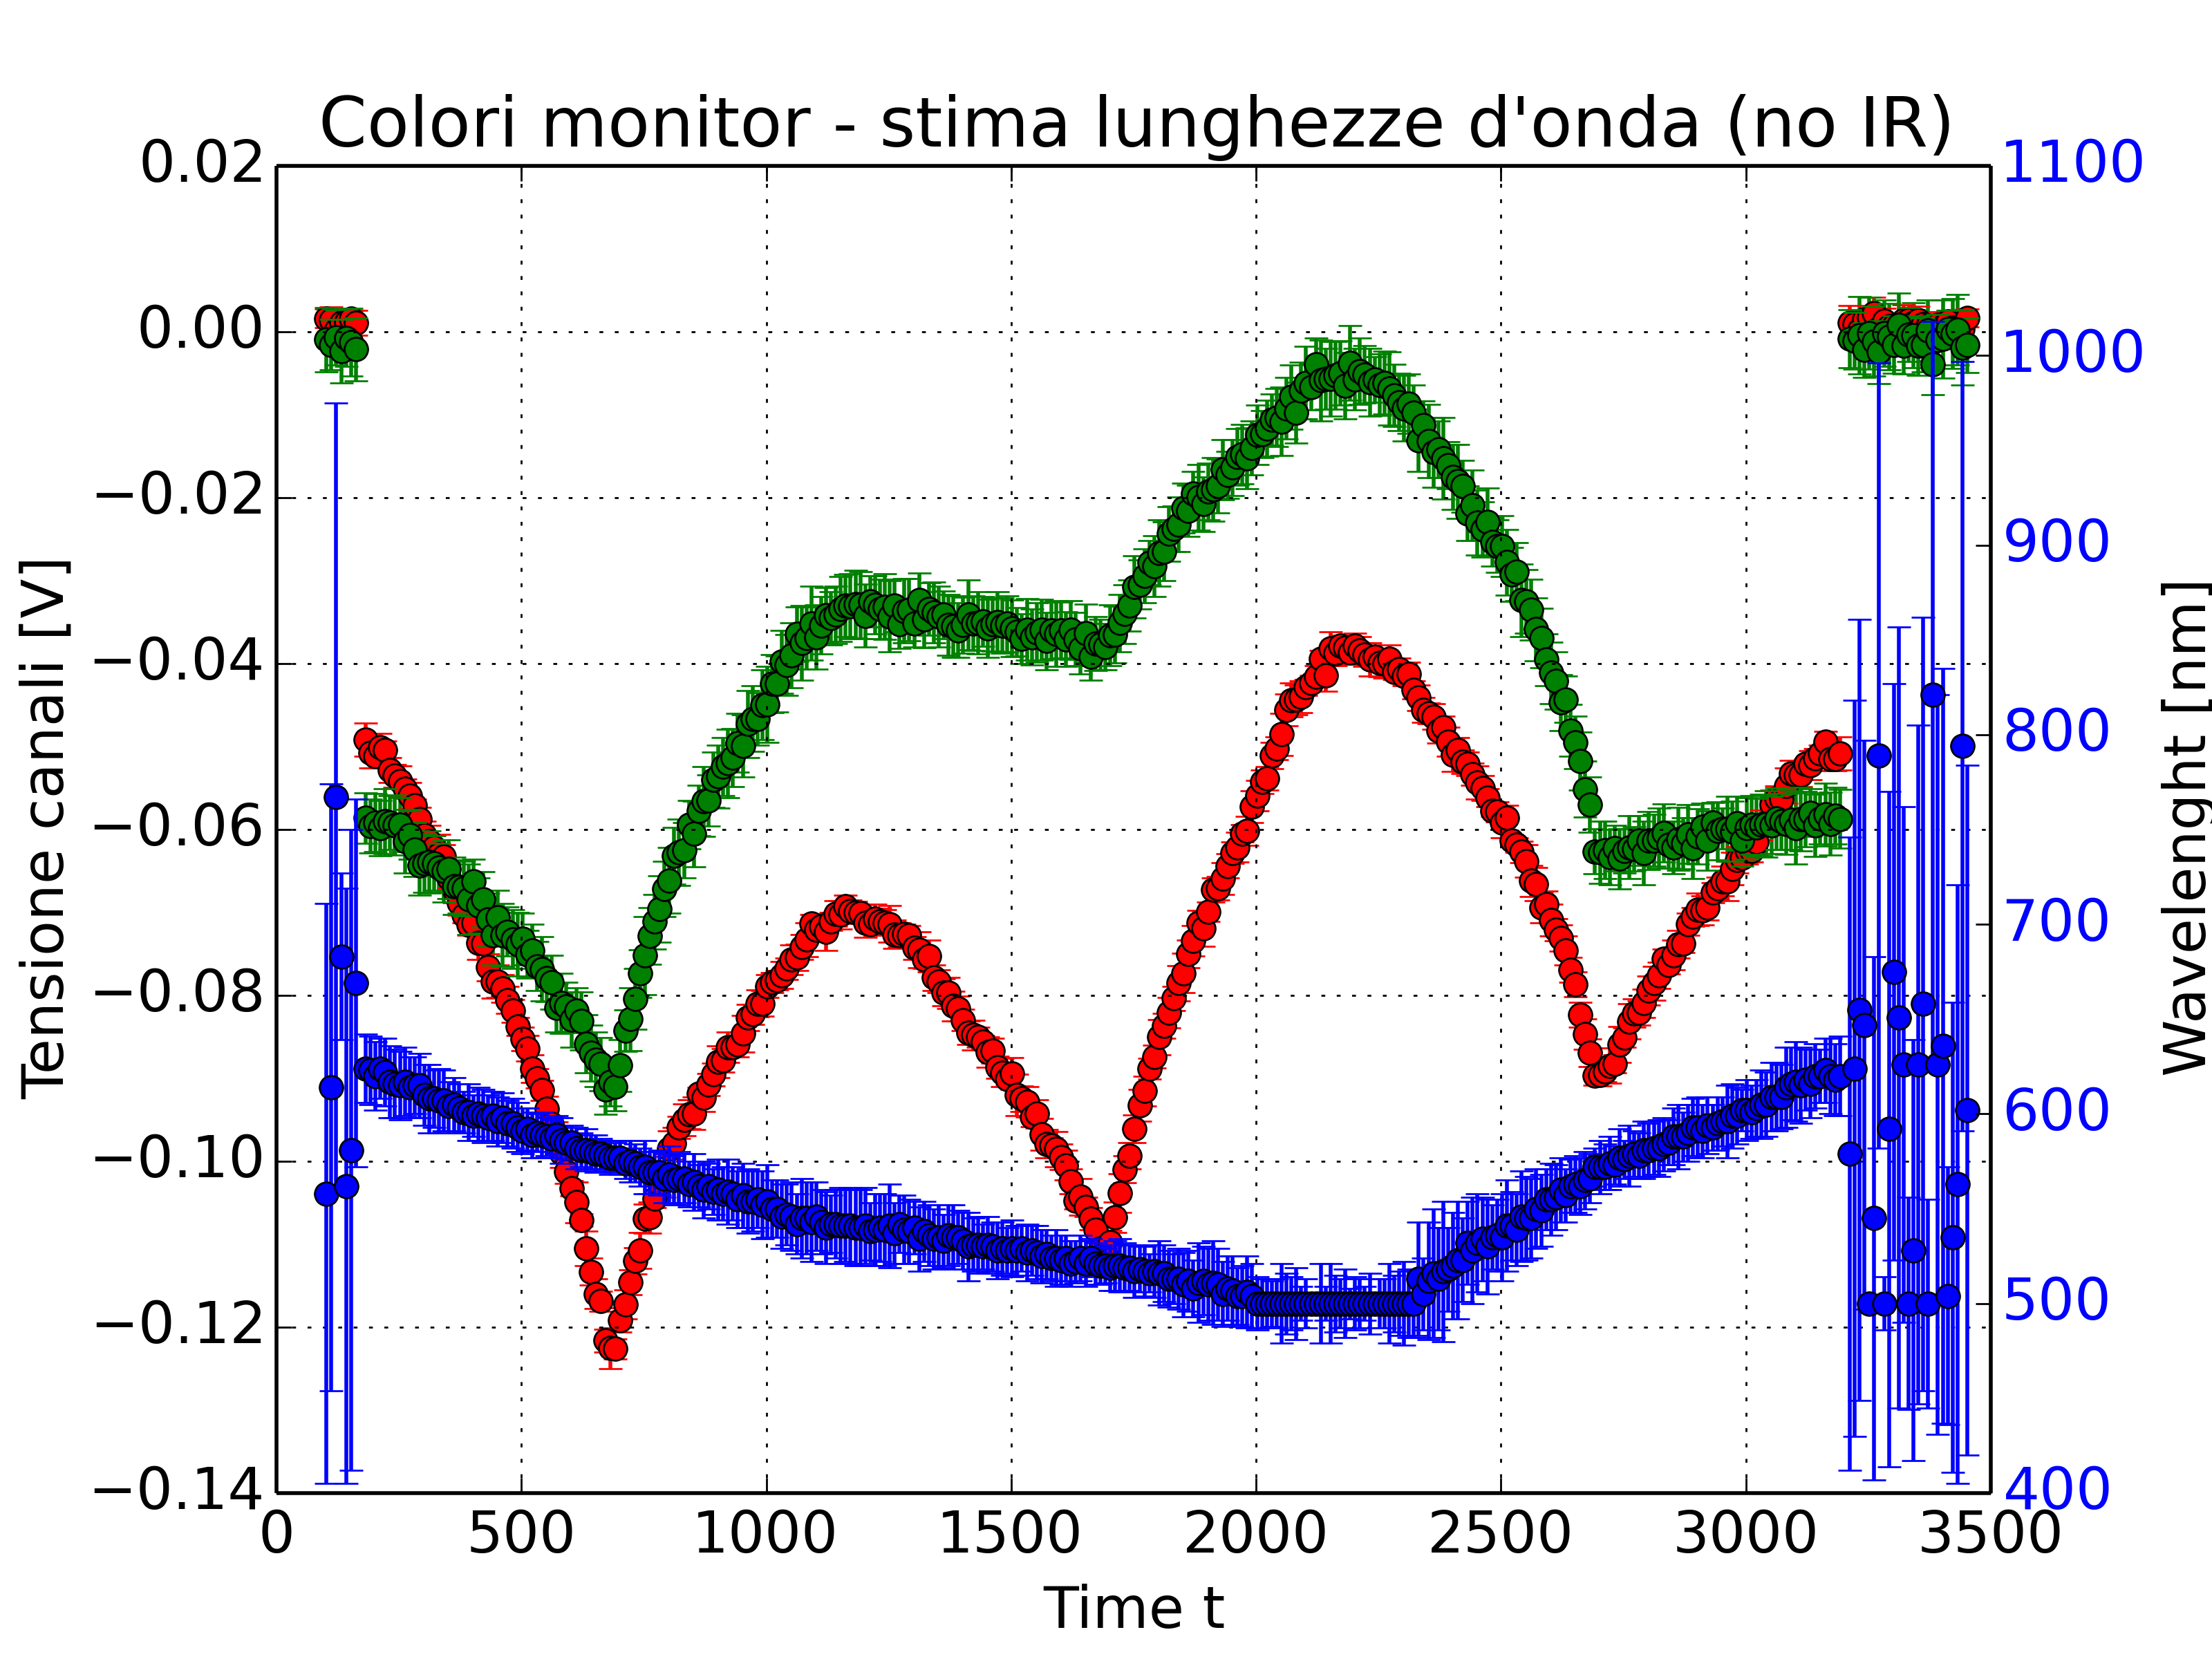
\includegraphics[width=0.6\linewidth]{./monitor_stima_lunghezzaonda_senzaIR}
%\caption{Stima della lunghezza d'onda a partire dal logaritmo del rapporto dei segnali, per ogni colore visualizzato sullo schermo, senza IR}
\label{fig:monitor_stima_lunghezzaonda_senzaIR}
\end{figure}

\begin{table}[h]
\centering
\begin{tabular}{c|c|c|c}
  & \textbf{RED} & \textbf{GREEN} & \textbf{BLUE} \\ 
 \hline Wavelength (nm) & 627(18) & 538(15) & $<$500(20) \\
 Colour ranges (nm) & 620-750 & 495-570 & 450-495 \\ 
\hline 
\end{tabular} 
\caption{Lunghezza d'onda dei colori puri RGB - no IR}
\label{RGB_lambda_noIR}
\end{table}
\end{frame}

\begin{frame}
\begin{itemize}
\item Il rosso è rimasto più o meno fisso.
\item Per il verde corrispondenza molto migliore e quasi coincidente con un verde puro.  
\item Blu saturato a 500nm: usiamo la curva di calibrazione estrapolata.
\end{itemize}
\end{frame}

\begin{frame}
\begin{figure}
\centering
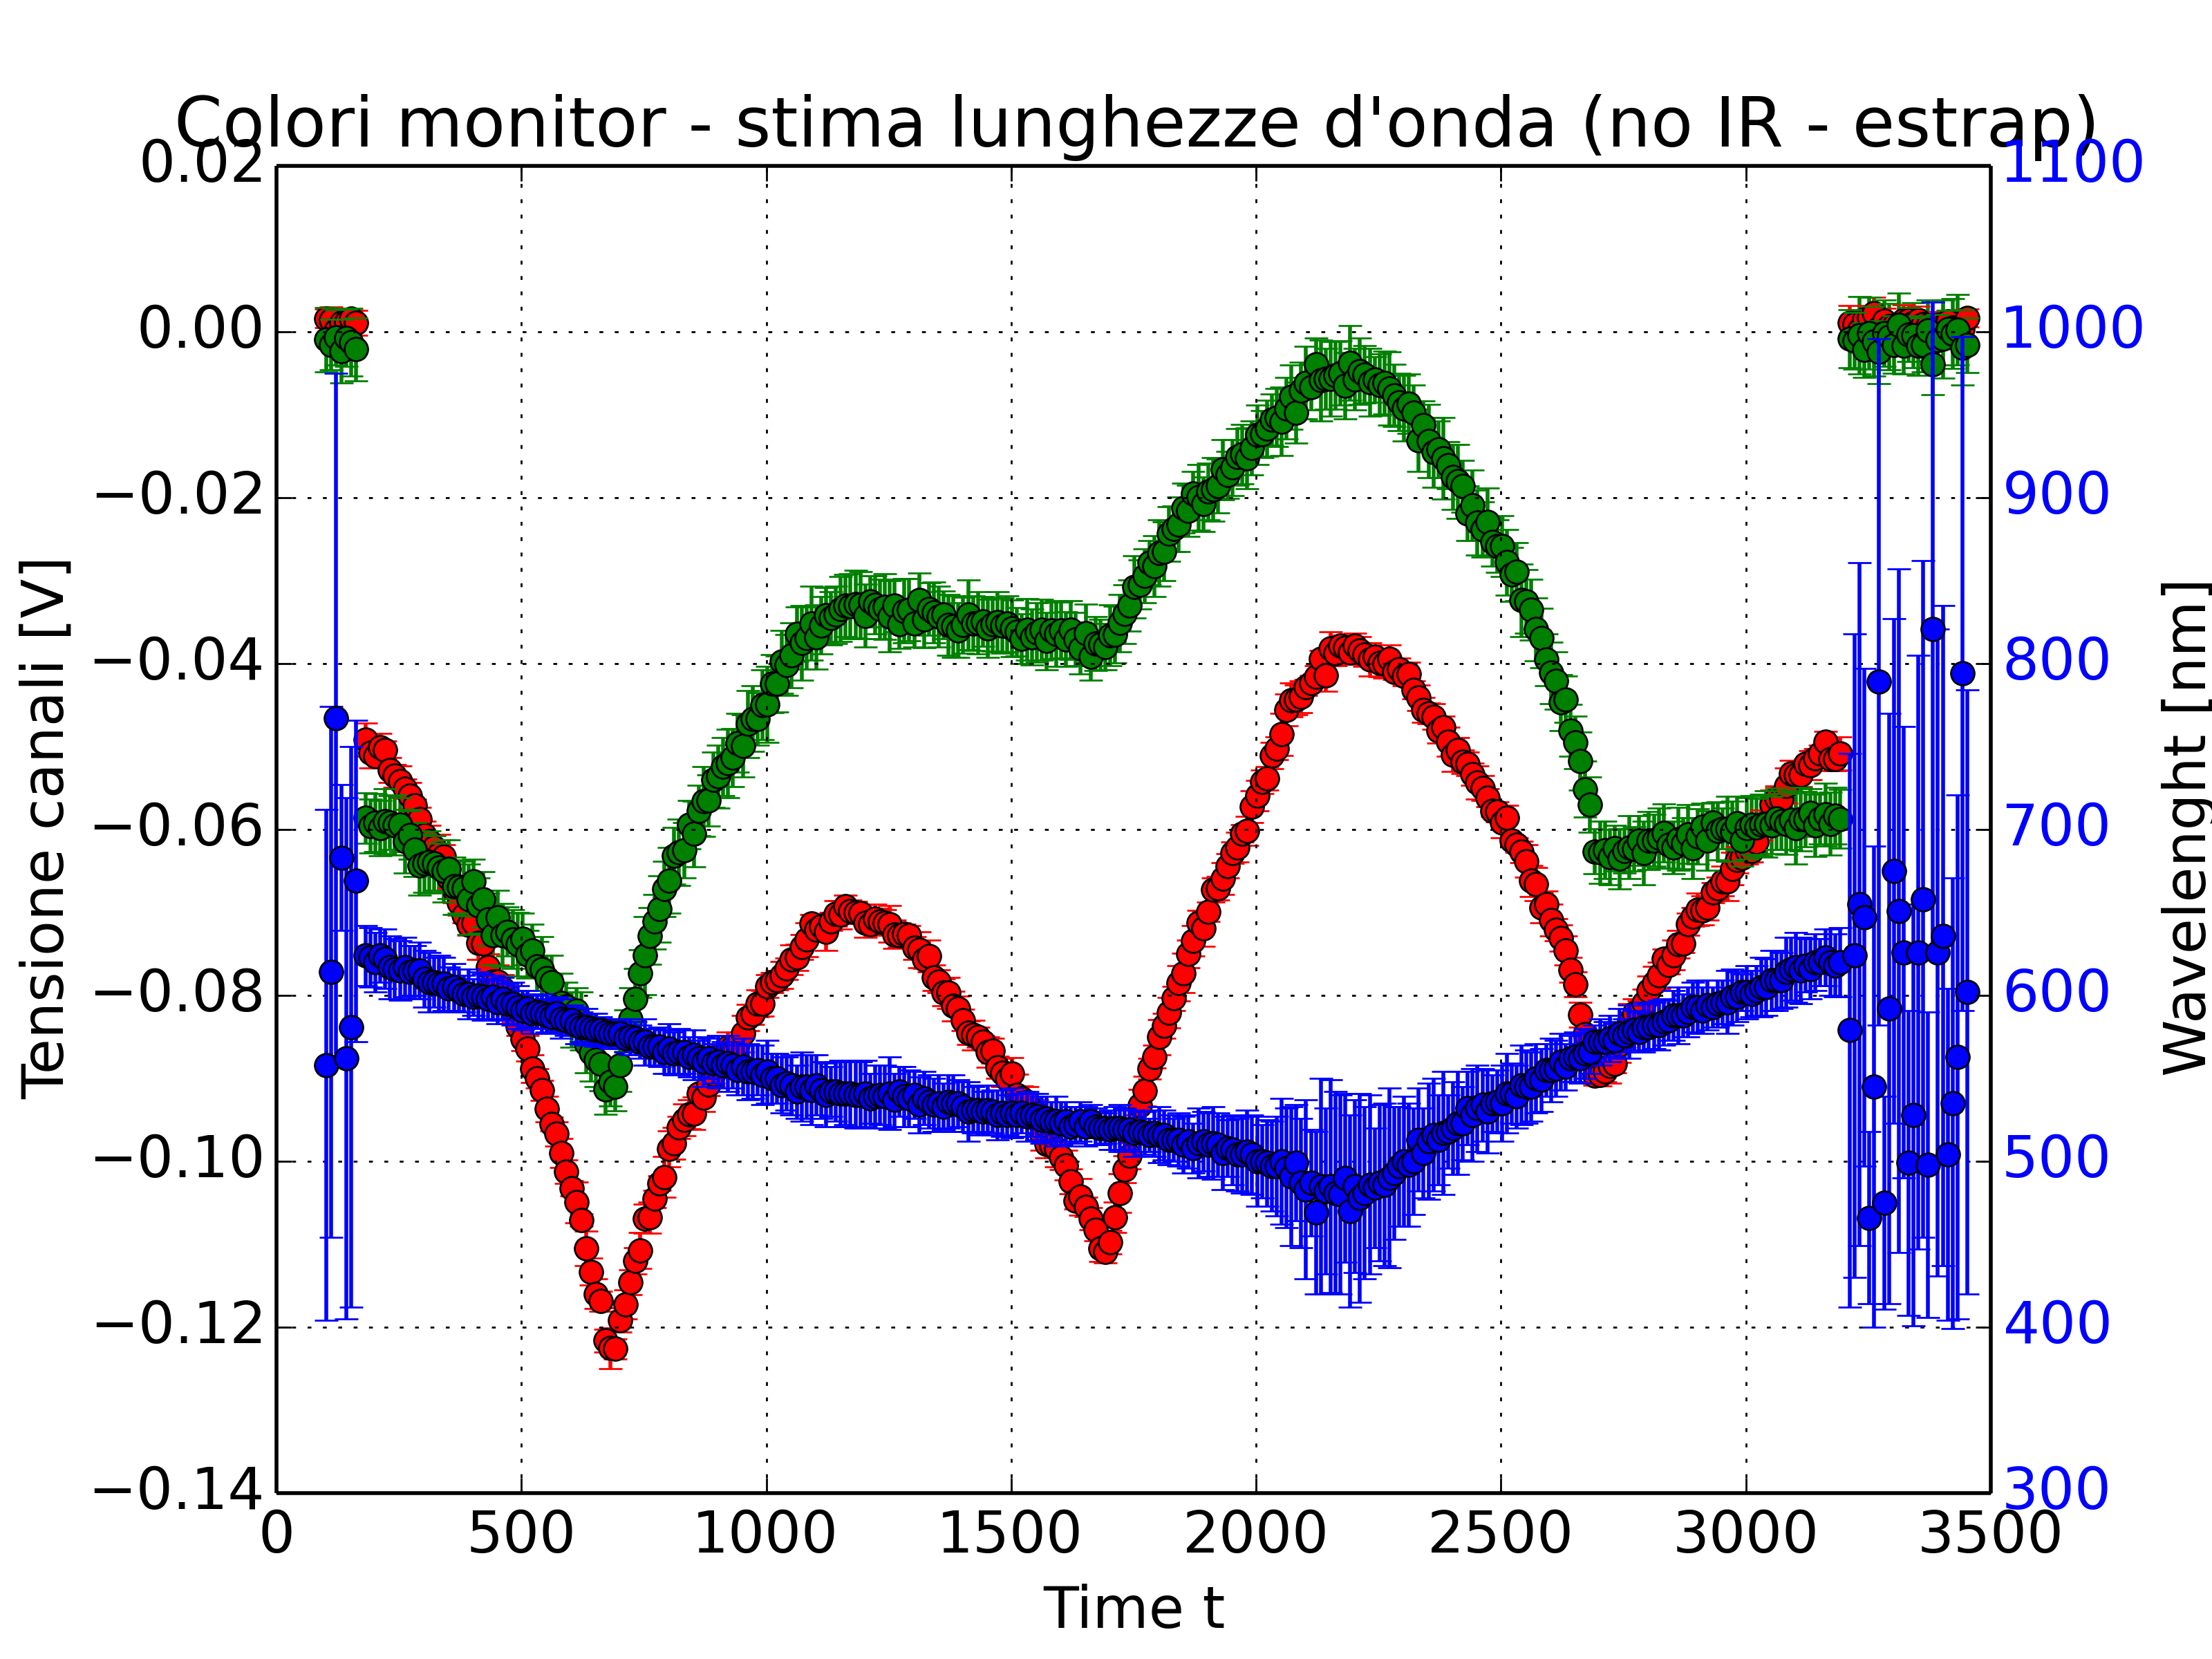
\includegraphics[width=0.6\linewidth]{./monitor_stima_lunghezzaonda_senzaIR_extended}
%\caption{Stima della lunghezza d'onda del monitor: senza fondo IR ed usando la curva di calibrazione "estesa".}
\label{fig:monitor_stima_lunghezzaonda_senzaIR_extended}
\end{figure}

\begin{table}[h]
\centering
\begin{tabular}{c|c|c|c}
  & \textbf{RED} & \textbf{GREEN} & \textbf{BLUE} \\ 
 \hline Wavelength (nm) & 627(18) & 538(15) & 470(50) \\
 Colour ranges (nm) & 620-750 & 495-570 & 450-495 \\ 
\hline 
\end{tabular} 
\caption{Lunghezza d'onda dei colori puri RGB - no IR}
\label{RGB_lambda_noIR_ext}
\end{table}
\end{frame}

\begin{frame}
\begin{itemize}
\item Il rosso e il verde sono (ovviamente) rimasti gli stessi, in buon accordo con le lunghezze d'onda effettive.
\item Finalmente il blu risulta avere una $\lambda$ decisamente buona, circa a metà dell'intervallo di definizione.
\item Errore considerevole sul blu dovuto alla bassissima responsività del fotodiodo 2 a lunghezze d'onda fra 400-500 nm: errore percentuale affatto trascurabile.
\item Significatività del BLU garantita dai LED.
\end{itemize}
\end{frame}

\begin{frame}{Gamut}
\begin{figure}
\centering
\label{fig:8_CIExy1931_sRGB_gamut_D65}
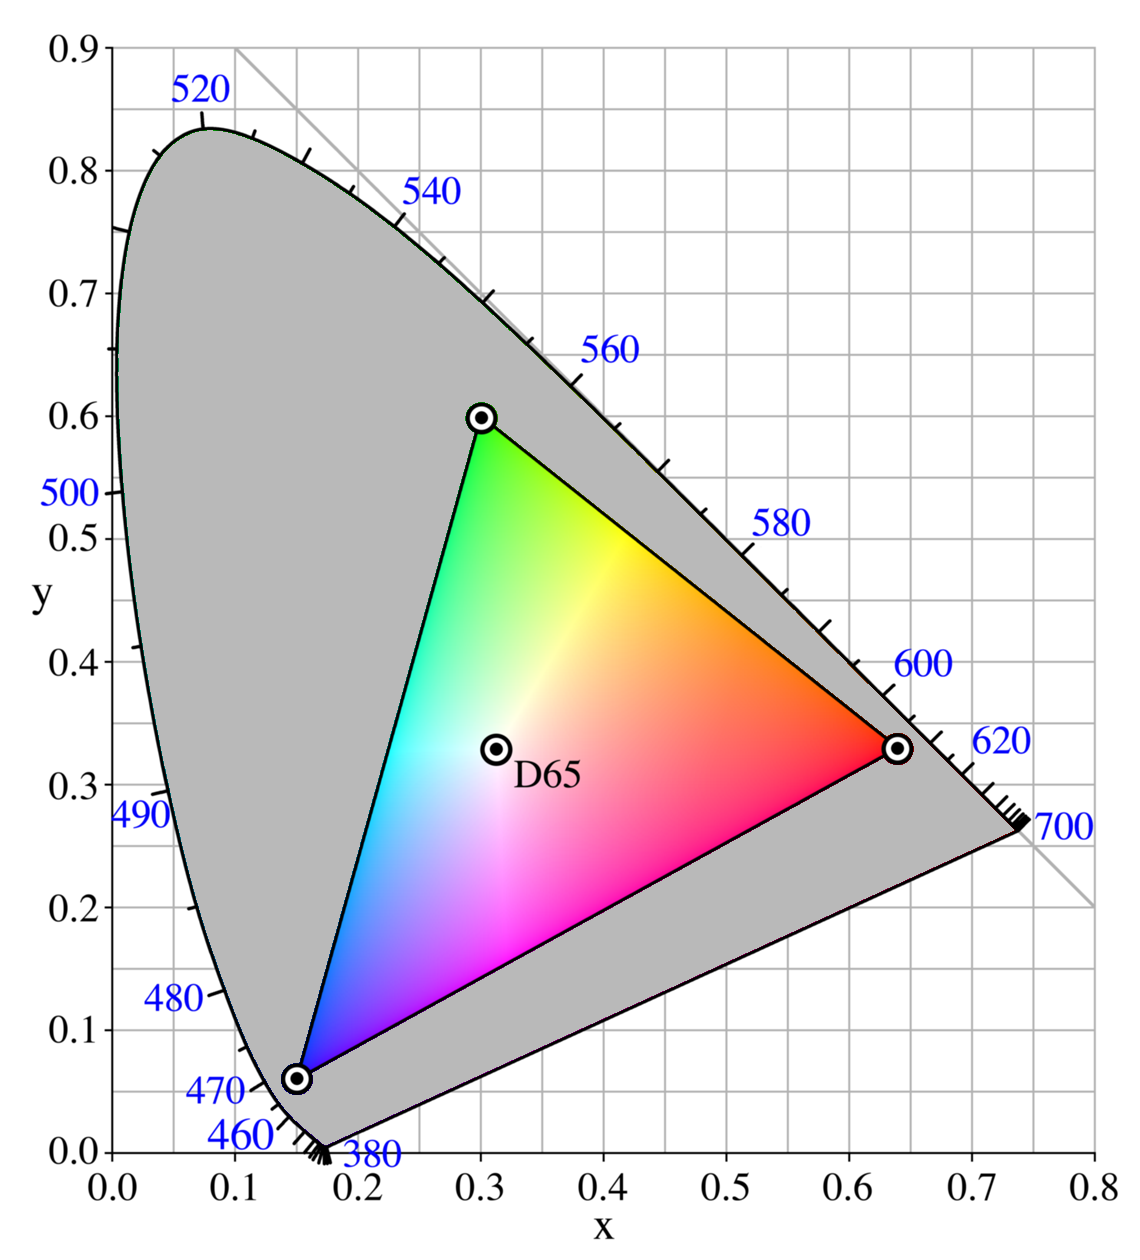
\includegraphics[width=0.55\linewidth]{./8_CIExy1931_sRGB_gamut_D65}
\end{figure}
\end{frame}

\begin{frame}{Tristimulus Functions}



\begin{textblock}{12}(-1.5,4)
\begin{figure}
\centering
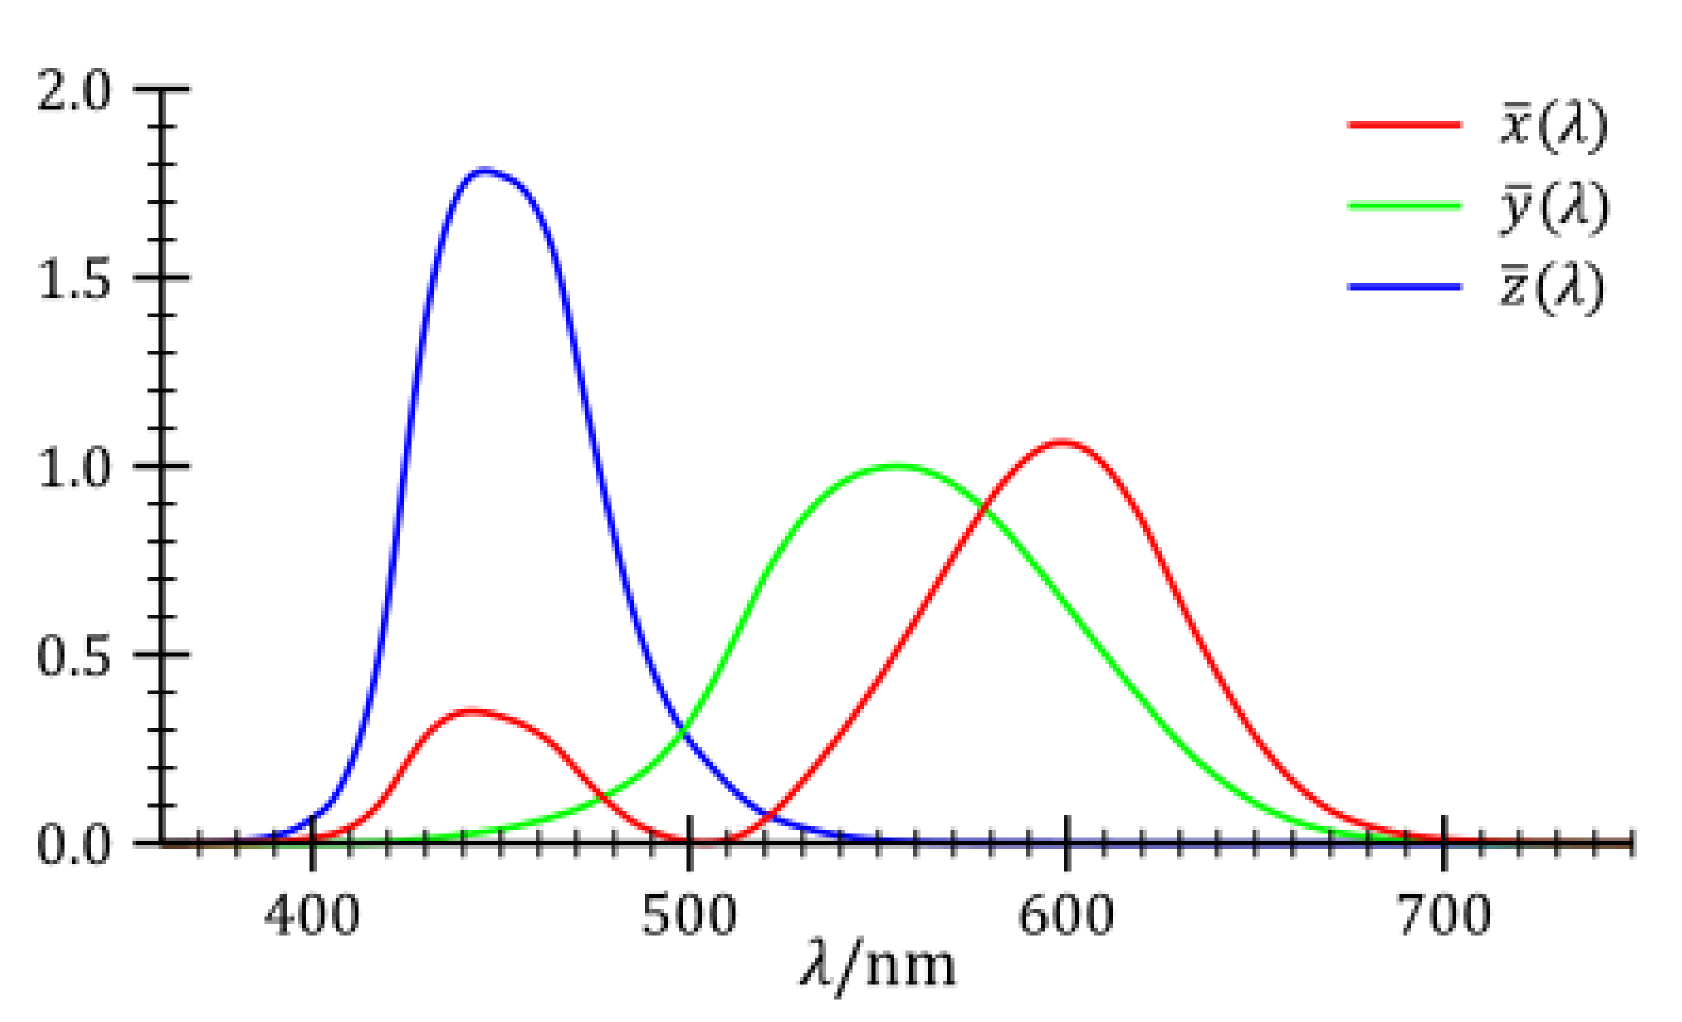
\includegraphics[width=0.7\linewidth]{./match_fun}
\label{fig:446px-CIE_1931_XYZ_Color_Matching_Functions}
\end{figure}
\end{textblock}


\begin{textblock}{8}(7,4)
\begin{equation}
\mathrm{X} = \int_{380}^{780} M(\lambda) \bar{x}(\lambda) \mathrm{d} \lambda
\end{equation}

\begin{equation}
\mathrm{Y} = \int_{380}^{780} M(\lambda) \bar{y}(\lambda) \mathrm{d} \lambda
\end{equation}

\begin{equation}
\mathrm{Z} = \int_{380}^{780} M(\lambda) \bar{z}(\lambda) \mathrm{d} \lambda
\end{equation}
\end{textblock}

\end{frame}

\begin{frame}{Luminosity Function - X}

\begin{itemize}
\item $\bar{x}(\lambda)$, $\bar{y}(\lambda)$ e $\bar{z}(\lambda)$ si definiscono \emph{colour matching functions}. 
\item Le colour matching functions sono definite in modo tale da riprodurre la responsività dei tre tipi di coni presenti nell'occhio.
\item In particolare la $\bar{y}(\lambda)$ è detta \textit{luminosity function}: descrive la sensitività spettrale media della percezione visuale della luminosità (da parte dell'occhio umano).
\item Qualitativamente la tristimulus function X (definita prima) rappresenta la percentuale di rosso che compone la radiazione incidente. 
\end{itemize}
\end{frame}

\begin{frame}{Cella fotovoltaica}
\begin{figure}
\centering
\label{fig:dati_normal}
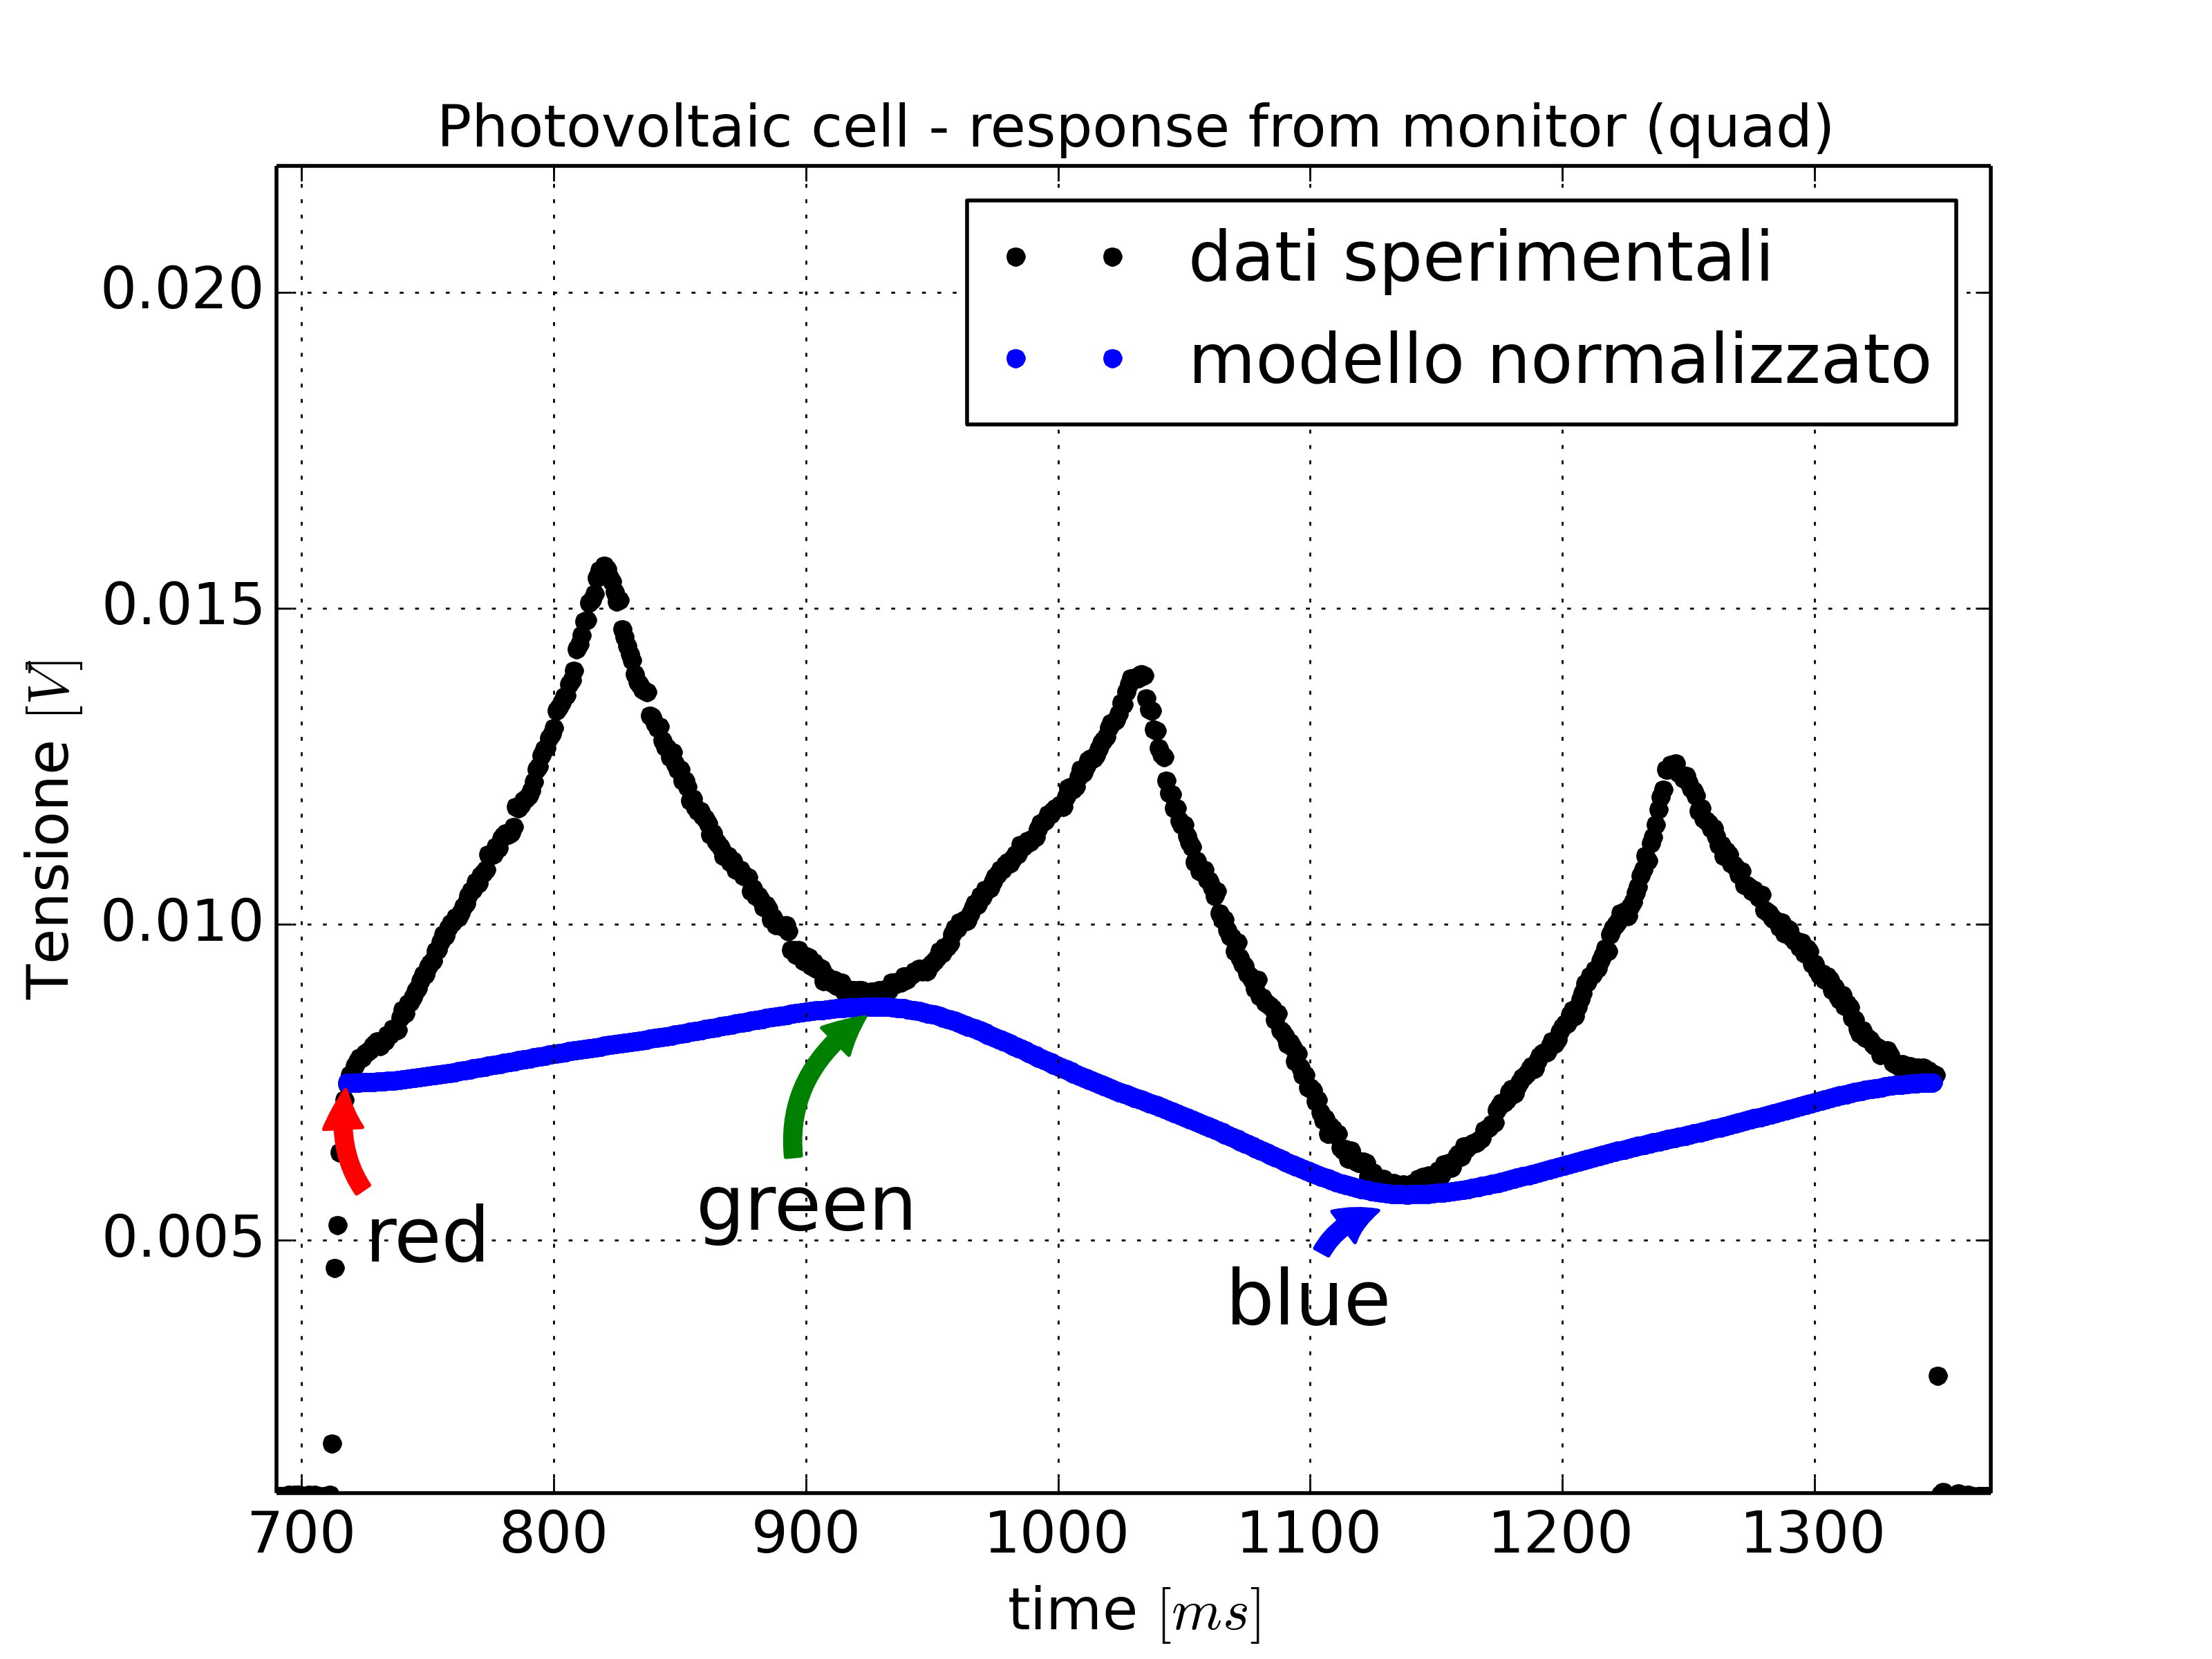
\includegraphics[width=0.55\linewidth]{./dati_normal}
\end{figure}

\begin{itemize}
\item Con il modello quadratico avevamo ricavato le intensità relative dei colori puri.
\item Adesso siamo in grado di assegnare un valore di "pseudo-wavelength" per ogni tripletta.
\end{itemize}

\end{frame}

\begin{frame}{Coincidenze? Noi crediamo di no.}

\begin{textblock}{12}(-1.5,4)
\begin{figure}
\centering
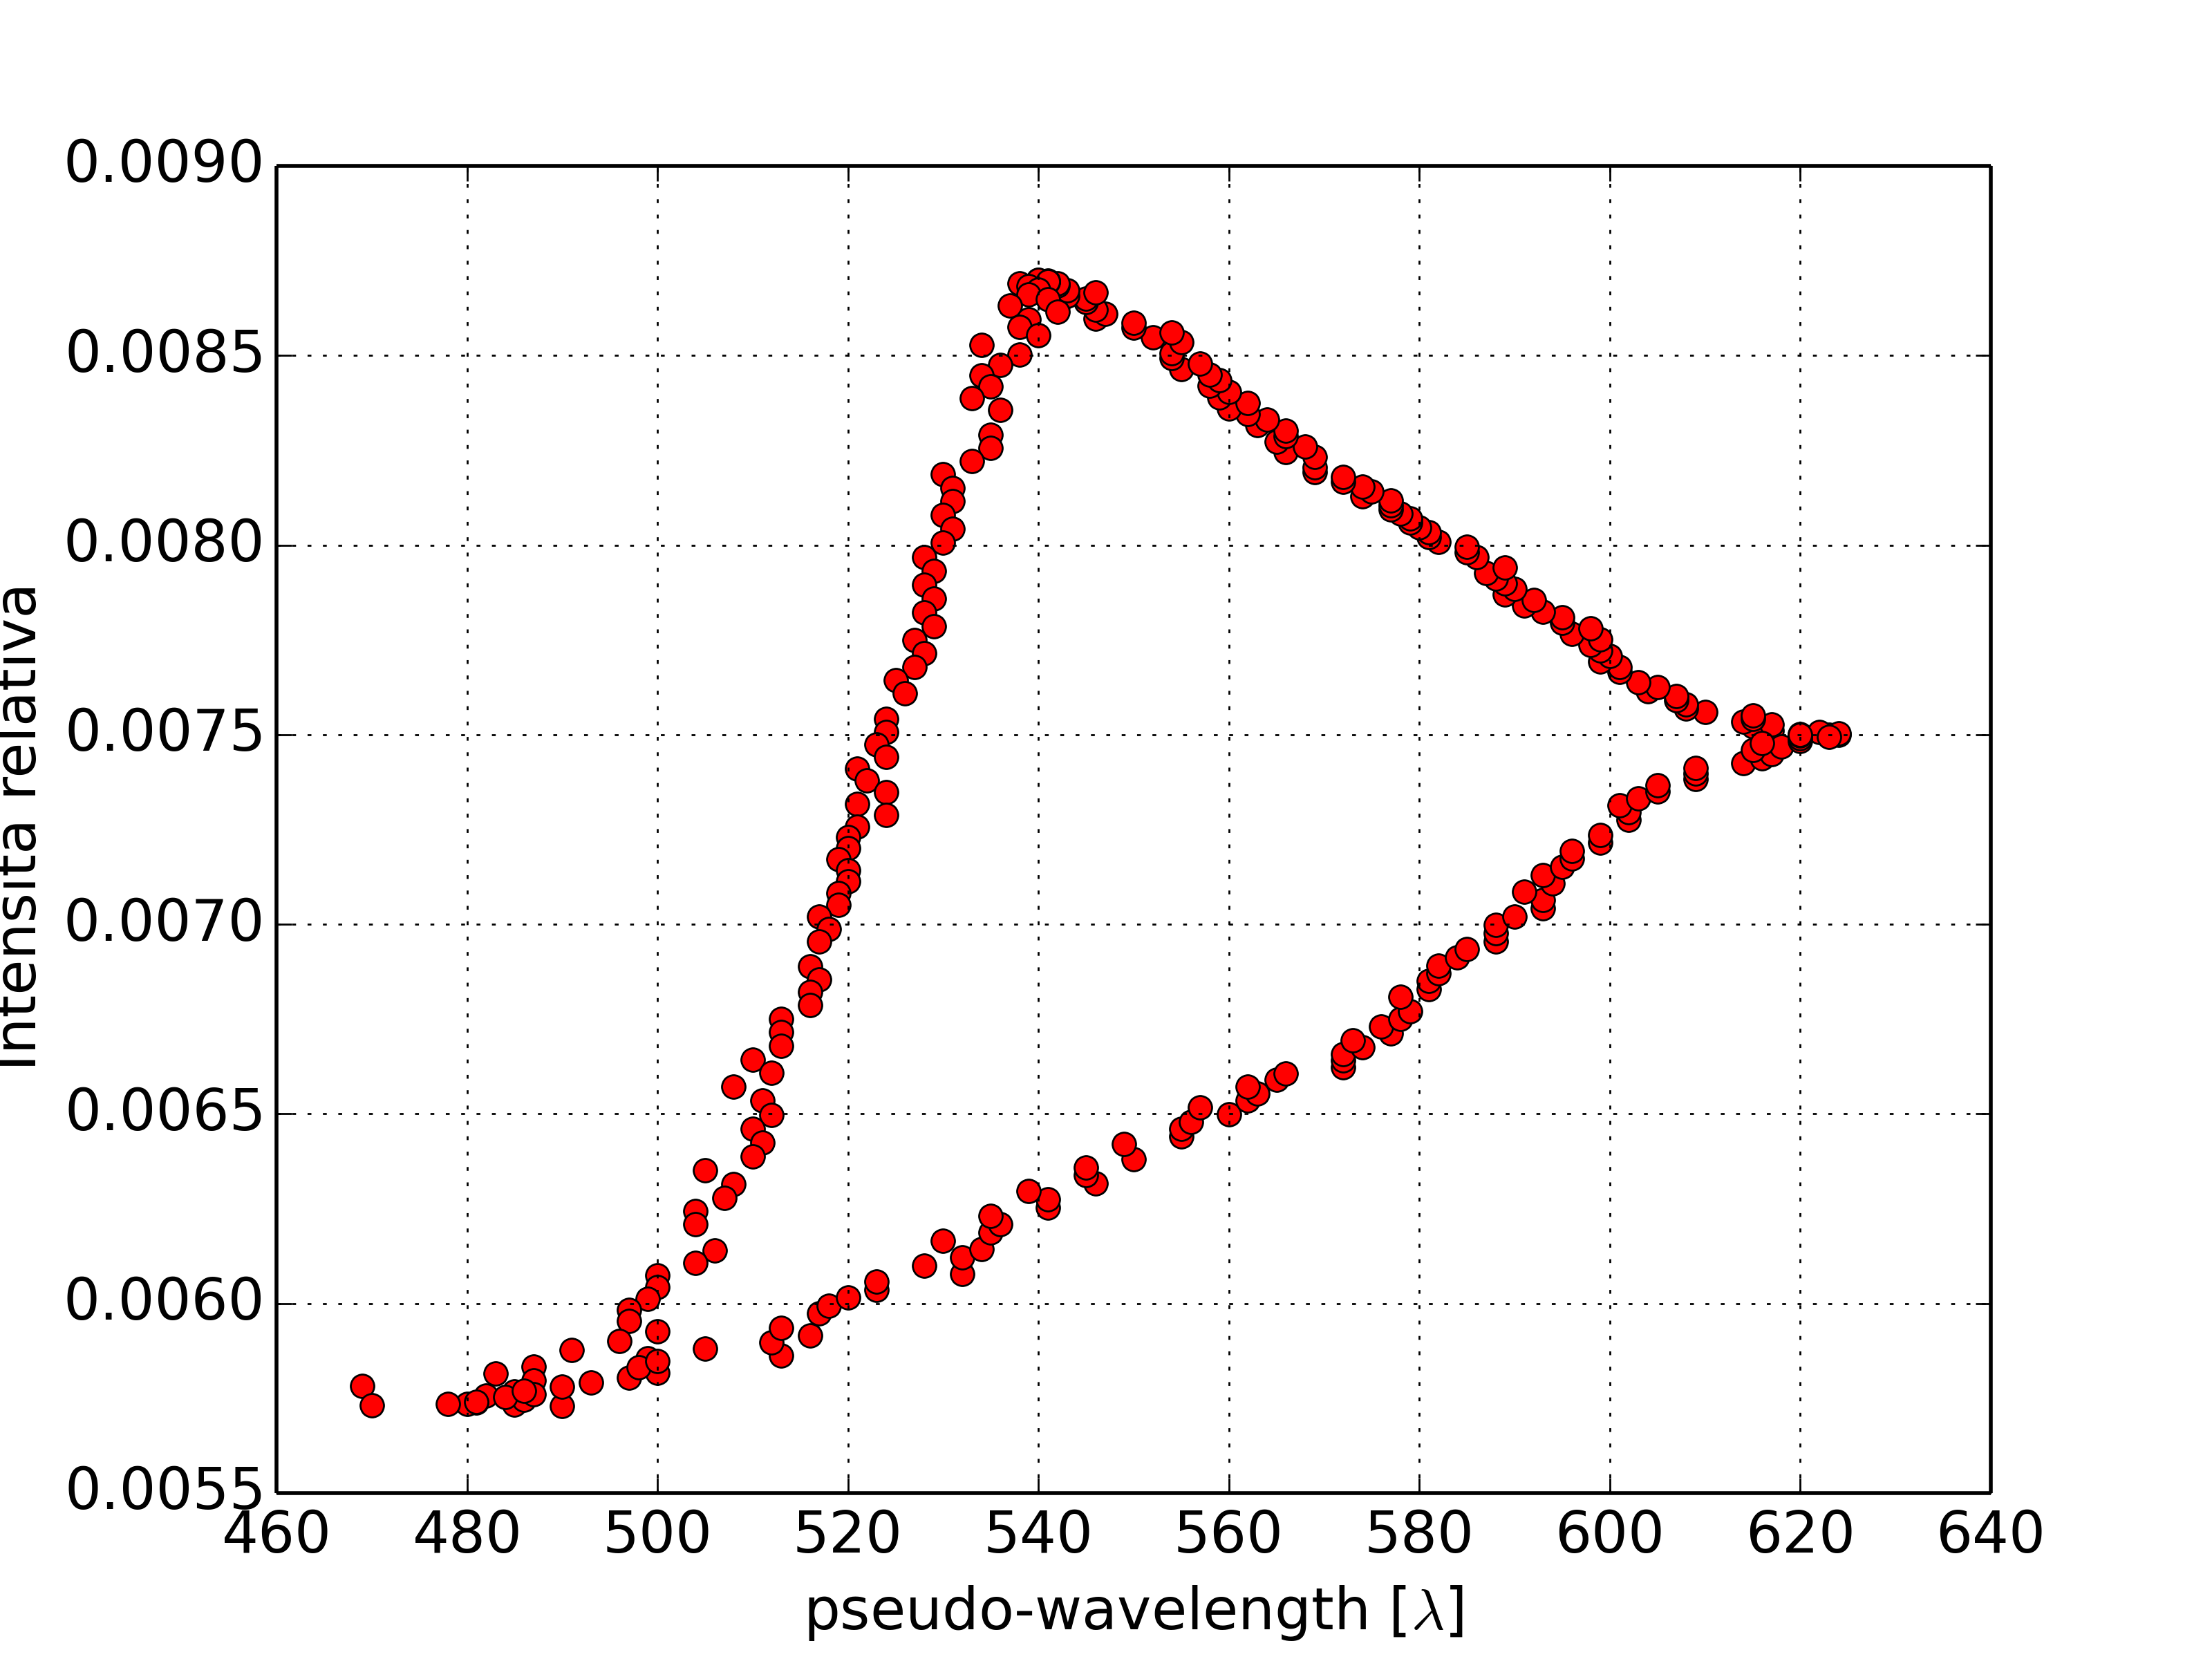
\includegraphics[width=0.7\linewidth]{./nostro_gamut}
\label{fig:nostro_gamu}
\end{figure}
\end{textblock}


\begin{textblock}{12}(6,4)
\begin{figure}
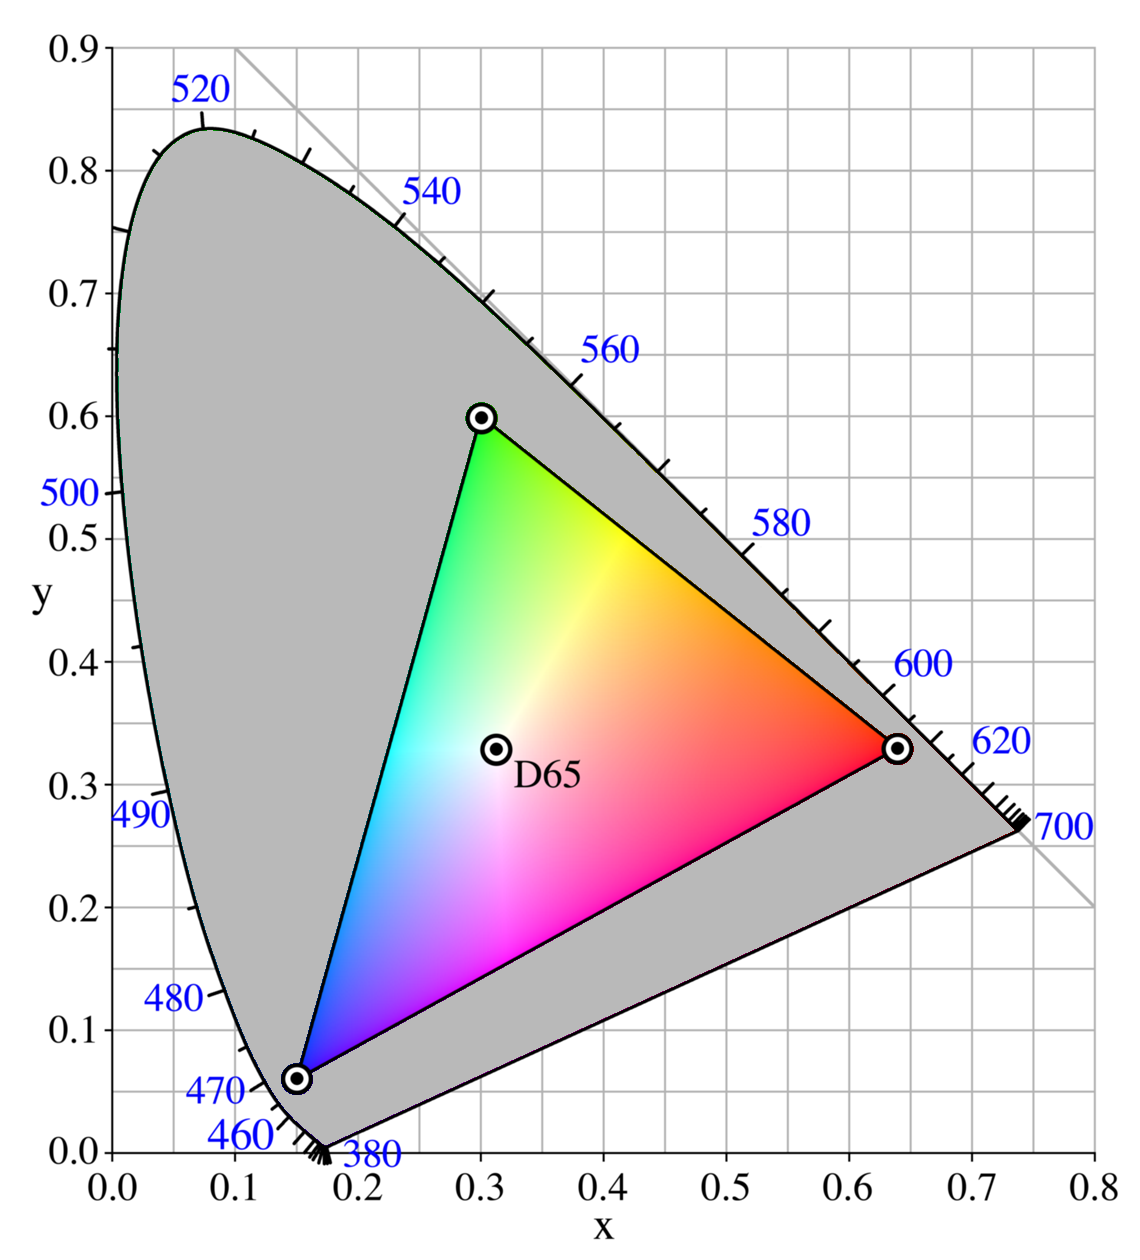
\includegraphics[width=0.45\linewidth]{./8_CIExy1931_sRGB_gamut_D65}
%\label{fig:cal}
\end{figure}
\end{textblock}

\end{frame}

\begin{frame}
\begin{itemize}
\item Nel nostro grafico l'asse y corrisponde alla luminosità relativa dei colori $\leftrightarrow$ asse y del gamut.
\item L'asse x del gamut è una misura di quanto rosso è presente nella radiazione e questa quantità aumenta andando da sinistra a destra. Incidentalmente la nostra pseudo lunghezza d'onda classifica a sua volta i colori RGB in base allo stesso criterio poichè procedendo verso $\lambda$ maggiori ci avviciniamo al colore rosso.
\item Con questo non vogliamo dire le le scale coincidono, ma che è possibile stabilire fra le due una certa corrispondenza qualitativa.
\item In questo modo abbiamo ottenuto il gamut per i colori RGB.
\end{itemize}
\end{frame}

\end{document}